\documentclass[12pt]{report}

\providecommand{\E}[1]{\ensuremath{\times 10^{#1}}}
\usepackage{graphicx}% Include figure files
\usepackage{amsmath}
\usepackage{amsfonts}
\usepackage{amssymb}

\usepackage{natbib}
%\bibliographystyle{ieeetr}
\bibliographystyle{agufull08}
\setcitestyle{authoryear, square}

\usepackage{cleveref}
%\usepackage{caption}
\usepackage{subcaption}





% Vectors in bold font instead of line over
\renewcommand{\vec}[1]{\mathbf{#1}}
% Math-mode vector alternative (greek symbols)
\newcommand{\mvec}[1]{\boldsymbol{#1}}

% units in math mode
\newcommand{\unit}[1]{\quad[\mathrm{#1}]}

% Big fractions
\newcommand{\bigfrac}[2]{\ensuremath{\frac{\displaystyle #1}{\displaystyle #2}}}


% Exponential:
\renewcommand{\exp}[1]{e^{#1}}
\usepackage{suthesis-2e}
    \specialthesis

\dept{Electrical Engineering}


    \begin{document}
    \title{Global and Seasonal Effects of\\
            Lightning-Induced Electron Precipitation}
    \author{Austin Patrick Sousa}
    \principaladviser{Prof. Sigrid Close}
    \firstreader{Prof. Robert Marshall, University of Colorado Boulder}
    \secondreader{Prof. Antony Fraser-Smith} 
    \beforepreface
    \prefacesection{Preface}
        This thesis tells you all you need to know about...
    \prefacesection{Acknowledgments}
        This dissertation represents the culmination of my nearly seven years at Stanford, and I've been thinking about writing this section for the last three. And yet, sitting here at my desk at the University of Colorado, I find myself at a lack for words.

Going into a Ph.D program, you tend to think of a dissertation as a final, be-all, end-all answer, a pinnacle of unrelenting, focused, thoughtful research, culminating in The Great Answer to your questions. Now, at the end of my program, however, this dissertation feels oddly anticlimactic. My path to this point was by no means direct: graduate research is by nature a meander, a random walk trajectory through courses and projects and countless research papers. There's no straight line to the finish - but there is, with enough guidance, a drift. 

By no means would I say I've arrived at the fabled ``answer''. I don't feel a sense of enlightenment. My work here has left me with an ever-expanding set of questions, model improvements, approximations and assumptions in need of scrutiny. But in a sense that is the destination for the countless hopeful academics who have embarked on a Ph.D. At the end, there are only more questions.

My particular path through Stanford was not direct at all. I entered as a first year student in the VLF group, which focused on low-frequency radio waves in the magnetosphere. The VLF group was built on over 50 years of geophysics and radioscience research at Stanford, and consisted of a thriving collection of a half-dozen research staff and nearly twenty graduate students, under the direction of Dr. Umran Inan. I knew early on that the VLF group had reached the end of its lifespan going into it, but had been assured that things would continue smoothly, that there would be people to work with, and that I would be one of a handful of final students to carry the VLF banner.

Within my first couple years, I worked on several interesting and unique research opportunities -- beginning first with hardware design for a CubeSat (see chapter \ref{chapter:vpm}),

VLF waves traverse great distances, and research on these waves follows accordingly. The VLF group prided itself on maintaining a global network of student-maintained radio receivers, from Alaska to Antarctica. Less than two years in as a student, I found myself, along with fellow student Chris Young, dragging four heavy Pelican cases through the rush-hour crush of a train station in Kagoshima, Japan, as part of a ten-day stint installing three such receivers in Sapporo, Kagoshima, and Mt. Fuji. Similarly, I had been entrusted, along with a handful of other students, with designing a CubeSat -- which would go to space! -- which at the time felt both incredible and overwhelming. The excitement within the group was palpable, fueled by a driven professor and supported by the well-trained machinery of the senior research staff.

Unfortunately, things were somewhat built to spill, and as the quarters progressed steadily on, our ranks began to dwindle. Other groups brought in new students and new projects; but I was the last one in the door. The excitement dwindled; the research meetings grew smaller and smaller. Labs were shut down, equipment surplussed, and the open doors of professors remained frequently shut. 

As the group continued to shrink, my research advisor, Dr. Sigrid Close, graciously took me into her lab in the Aerospace Engineering department, along with VLF research scientists Dr. Robert Marshall and Dr. Ivan Linscott. Switching to the AA department was a fantastic opportunity to escape the loneliness and gloom of the Packard basement lab. Courses and research continued on, now in an active research group (and with daylight windows!). Not soon thereafter, however, Dr. Robert Marshall secured a coveted faculty position at CU Boulder. I found myself working on a project unrelated to my fellow students, and again lacked an in person mentor.

The fourth year was the hardest. By four years in, you've likely taken all the classes you need to, and hopefully have a start on a dissertation topic. But by four years, you're too far in to quit, and yet the end is nowhere in sight. Furthermore, with no remaining classes to count, you're truly cut free -- and without steady guidance, there's no obvious way forward.

-----------

There are countless people who, without their invaluable guidance, I would not be writing this section today. First and foremost, to my mentor, Dr. Robert Marshall, who has been perhaps the one constant thread throughout my seven years, first as a faculty mentor on the VPM project, then as a co-advisor in the AA department, and now as my PI at the University of Colorado. Bob, you're an inspiration.

To my advisor, Dr. Sigrid Close, who took me in despite having an already overwhelming cadre of students. I've always appreciated our conversations, and that you'd let them meander to topics across the board. As much as Bob would hone ideas in, Dr. Close would let brainstorming sessions run rampant.

To Dr. Antony Fraser-Smith, who as graciously served as my third committee member, especially while recovering from a heart surgery. Tony has been a part of the radioscience group at Stanford since the 1970s, and is a wellspring of interesting stories, entertaining anecdotes, and exudes the good-natured, jovial personality that makes geoscience a compelling world to work in. Furthermore, Dr. Fraser-Smith was responsible for putting together the Villard Fellowship for Students in Radioscience, in memory of the late Dr. Oswald Villard, which supported my first year of research, and was the deciding factor in my attending Stanford. 

To the researchers and engineers who kept the VLF group running: Dr. Ivan Linscott, Dr. Dave Lauben, Dr. Morris Cohen, who made themselves available for any and every question I had, no matter how trivial. A special thank you to Dr. Maria Spasojevic, who took the time to personally call me when I was applying to grad school.
 
To Jeff Chang, who singlehandedly ran every technical aspect of the VLF group, from the compute cluster to PCB layout to metal manufacturing.
 
To Professor Emiko Yasumoto in the Japanese language department, who showed special concern for my well-being during a particularly rough time. \begin{CJK}{UTF8}{min}??????????\end{CJK} \\

To my friends, colleagues, and lunch buddies from the VLF and SESS groups: Chris Young, with whom I've shared adventures across Japan; David Freese, for dragging me 5000 feet up Half Dome in the middle of the night; Patrick Blaes, who taught me everything I know about everything (no joke). To Rasoul Kabirzadeh, who started the same quarter as I did and went through many of the same struggles I encountered. To Nicholas, Sid, Anna, Lorenzo, and everyone in the SESS group who welcomed me in halfway through my program: Thank you all.

I owe a truly incalculable debt of gratitude to my community outside of campus, who without their constant companionship I most surely would have turned tail and returned to Seattle in 2012. To Ted Phares and Tristan Hudson, for 2am snacks and 2pm breakfast. To Damien Heiser and Wayne Tsai, for bringing me to Burning Man --Twice!\footnote{so far}. To Galen, Abe, JDT, Mike, Phil, Dan, Ricky, Hukka, Max, and everyone else: more than the classes, more than the research: you guys made me the person I am today, and I would not be here without you. Thank you.

To my former bosses and colleagues in the music industry, from my life before college, Bob Lang and Stuart Hallerman, for inspiring me to study electronics in the first place.

To my partner of nearly 9 years, Ty Logan: Thanks for putting up with me.

Finally, to my high school history teacher, Mark Rippy: In my senior year, I had to write a history paper and I refused to do it. Mark gave me some brief, offhand advice that hit me at just the right moment: ``Nobody else will do it for you." It was a bombshell, and it changed my life. It sounds silly, but those words became a mantra that got me through high school, an associate's degree, five years in the music industry, two bachelors degrees, a Master's degree, and now, a Stanford doctorate. Thank you.


    \afterpreface
 
    \chapter{Introduction}
    	\section{The Space Environment}
%Surrounding the Earth there exists a sparse gas of ions and electrons called a \emph{plasma}. 
The Earth is surrounded by a sparse gas of ions and electrons called a \emph{plasma}. 
These particles are in a state of constant motion, resulting from a tenuous and dynamic balance of energy fluxes -- streaming in from the sun, to and from the Earth's terrestrial atmosphere, and out into space. Every human-made satellite has passed through it; the vast majority of satellites, with the exception of deep-space probes, live out their entire existence within it. Aside from the lunar astronauts of the Apollo era, every single human in space has spent the duration of their journey within this constantly-evolving cloud of matter. The technology ubiquitous in our day-to-day lives -- instant international communication, satellite-aided global positioning systems -- all require signals to be transmitted through it. We call this region, from an altitude of 90 km all the way out to the moon, the \emph{space environment}.

%The space environment is defined largely by the Earth's magnetic field. We refer to this system as the \emph{Magnetosphere}, and the plasma contained within it as the \emph{Plasmasphere}. 

\begin{figure}[ht!]
\begin{center}
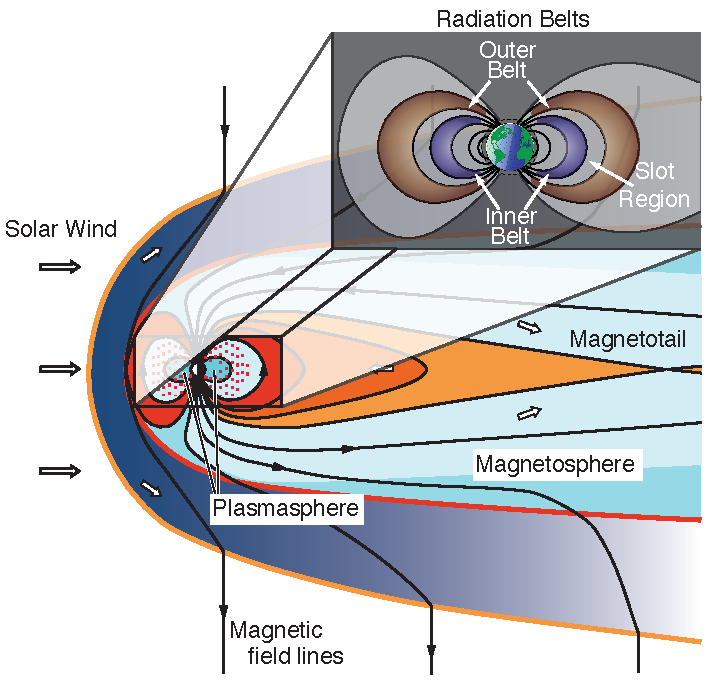
\includegraphics[width=0.8\textwidth]{figures/space_environment_figure.pdf}
\caption[Diagram of the various regions of the space environment]{The various regions of the near-Earth Space Environment. The topology of the space environment is driven by the Earth's magnetic field, and by the solar wind. The radiation belts are shown in the inset. Figure adapted from \cite{Graf2013}, which was adapted from \cite{Hill1991}.}
\label{fig:space_environment}
\end{center}
\end{figure}

The space environment is largely defined by the Earth's magnetic field, which constrains the plasma to a toroidal shape. The region in which the Earth's magnetic is dominant over the interplanetary magnetic field is called the \emph{magnetosphere}, and the region of constrained plasma immediately surrounding the Earth is called the \emph{plasmasphere}. The majority of the particles within the plasmasphere are cold, with kinetic energies less than $\sim$ 1 electronvolt (eV). However, a sparse population of high-energy particles exist, with energies ranging between 100 keV -- 10 MeV, and velocities approaching 99\% of speed of light. These so-called ``killer electrons", while sparse in number, present a significant hazard for both electrical systems, and to living organisms in space \citep{Barth2003}. The populations of these particles form two shells, known as the Van Allen radiation belts, separated by a depleted ``slot" region. Understanding the behavior of these high-energy particles are key to sustained human activity in space. 

The population of high-energy particles is driven by a complex balance of sources, acceleration mechanisms, and loss processes. This thesis considers the effect of one such loss mechanism: the action of radio waves generated by terrestrial lightning through a resonant scattering process known as \emph{Lightning-induced Electron Precipitation} (LEP), and examines the regions of the space environment in which losses due to LEP may be substantial. We perform this study through extensive numerical simulation of single LEP events, under a variety of space weather conditions, and examine global trends by extrapolating over a global lightning activity dataset.



\section{Motivation}
\subsection{The Radiation Belts}
The Van Allen radiation belts, first measured in 1958 by \cite{VanAllen1958} on the Explorer I and III satellites, represent one of the earliest major discoveries of the American space program. The belts are an enhancement in very-high-energy particles (E $>$ 100 keV), which extend from 1.2 to 7 earth radii ($\sim$ 7,500 to 50,000 km) along the equator, and follow the Earth's magnetic field to $\sim \pm65^\circ$ latitude, as shown in the inset in Figure \ref{fig:space_environment} \citep{Walt1994}. While the location and population of the belts are highly dynamic, it is customary to divide the population of high-energy particles into two toroidal shells: an inner belt below $\sim$ 3 Earth radii and an outer belt between $\sim$ 3 and 7 Earth radii, separated by a ``slot" depletion region between 2 and 3 Earth radii. The radiation belts are dominantly populated by electrons ($e^-$) and protons (hydrogen ions, $H^+$). Geomagnetically-trapped particles are confined by the Earth's magnetic field, and exhibit a helical bouncing motion, reflecting between fixed points near the northern and southern poles.

It was recognized early on that the ionizing effects of high-energy electrons represented a hazard for both humans and electronics in space. The Apollo manned spaceflight missions dealt with the risk of ionizing radiation both by incorporating additional aluminum shielding, and by designing their orbit trajectory to minimize time spent in the Van Allen belts \citep{Apollo1973}. Astronauts aboard the International Space Station wear passive dosimeters to measure total exposure, and have on occasion been required to take shelter in the innermost regions of the ISS, which are better shielded from the space environment, in the event of extreme solar or geomagnetic activity \citep{ugh}. 

As silicon gate sizes continue to shrink, electronics have become increasingly susceptible to radiation-related failures. Single-event upsets (SEU) can occur when a high-energy particle impinges on a volatile memory circuit, imparting enough energy to erroneously change a bit from 0 to 1, or 1 to 0. The effects of SEU can be mitigated through specialized design practices, including triple-redundant systems and larger gate sizes, and are regarded as `soft' failures from which a system can be designed to survive. Of additional risk are catastrophic failure events -- for instance, in which an energetic particle can impinge on the oxide layer of a FET transistor, and create an electrical short, either temporary or permanent. Such an event can render spaceborne electronics inoperable. Furthermore, the constant influx of charged particles can slowly degrade the doping of bulk silicon transistors, resulting in slower switching speeds and reduced gains through total-dose effects.

\subsection{Sources and Loss Processes}
The radiation belts are generally populated by the stream of particles arriving via the solar wind, which provides a steady flow of cold electrons (velocities $\sim 300$ km/sec, and temperatures $\sim 10^{-5}$ Kelvin) \citep{Montgomery1974, Tascione1988}. These particles are then gradually accelerated to relativistic energies through a variety of acceleration processes within the magnetosphere, such as resonant interactions with ULF waves, chorus waves, and magnetotail processes \citep{Shprits2006,  Bortnik2007a, Thorne2013}. The sources and acceleration mechanisms of radiation belt particles are active research topics; see the work of \cite{Jaynes2015} for an analysis of two filling events, and a multi-step process which may result in relativistic population enhancements.

The dynamics of the radiation belts are marked with periodic filling events, in which the distribution of high-energy particles rapidly increase \citep{Horne2005, Baker2014}. In the absence of other interactions, these particles would remain trapped by the Earth's magnetic field, and populations would continue to increase indefinitely. However the influx of new particles is balanced by an equally-complex set of loss processes.

Throughout the 1960s and 1970s, a wealth of research was performed on the lifetime of energetic radiation belt particles, most notably through a series of atmospheric nuclear detonations known as the \emph{Starfish} project\footnotemark. Starfish was a 1.4 megaton nuclear device, detonated 400 km above Johnson Island on July 9, 1962, which provided an artificial, local enhancement to the inner radiation belt at approximately 1.2 Earth radii \citep{Hess1963}. Data from particle detectors aboard several early satellites (Telstar, Injun, Ariel, and Tracc) were then used to study the lifetimes and dispersion characteristics of energetic protons and electrons. Starfish electrons were found to be very long-lived, with lifetimes on the order of $\sim 2$ years \citep{Beall1967}. Furthermore, in the months following the Starfish detonation, seven satellites, including Telstar 1, the first commercial communications satellite, which was launched one day after the Starfish detonation, experienced catastrophic failures \citep{Wenaas1978, Barth2003, Conrad2010}, inspiring a decades-long research interest in the lifetime of radiation belt particles, and anthropogenic techniques for the mitigation of nuclear-injected particles.

The earliest loss-mechanism theories considered Coulomb scattering against the nucleii of atmospheric neutral constituents \citep{Walt1964}. This model showed reasonable agreement with Starfish particles at the lowest altitudes ($\sim$ 1.1 Earth radii), but greatly overestimated particle lifetimes for the majority of inner-belt electrons, indicating that other, unaccounted-for loss processes must be present. 
\footnotetext[1]{While the Starfish detonation was the greatest yield and highest-altitude, and thus of the greatest interest in radiation belt physics, it was not by far an isolated event. Between 1955 and 1962, with a lapse following an international armistice between 1958 and 1961, the United States performed twelve atmospheric nuclear tests, at altitudes ranging from 6 to 540 kilometers, with yields in the kiloton range, reaching a maximum with Starfish at 1.4 megatons. Simultaneously, between 1961 and 1962, the Soviet Union performed five high-altitude detonations between 1.2 and 300 kilotons. An international moratorium on high-altitude detonations took place in 1963 with the High Altitude Nuclear Test Ban Treaty \citep{Hess1964b, Schwelb1964, Hoerlin1976, Norris1996}.}


\section{Previous Work}

\subsection{Wave-Particle Interactions}
Recognizing the need for additional loss mechanisms, It was soon theorized that resonant interactions with radio waves could significantly alter the reflection height of trapped particles, and in turn drive these particles further into the neutral atmosphere, where they stood a much higher chance of colliding with neutral constituents, and eventually precipitating into the neutral atmosphere. Unlike in free space, the charged medium of the plasmasphere allows propagation of only certain frequencies and modes of radio wave (see section \ref{section:waves_in_plasmas}). Right-hand, circularly-polarized waves in the VLF band ($\sim < 30 $ kHz) are common in the plasmasphere, and arise from a variety of generation mechanisms. These waves are known as \emph{whistlers}, named for the descending, whistle-like tones originating from distant, broadband impulses. Terrestrial lightning is a persistent source of whistlers, with $\sim$ 50 flashes/sec occurring globally; each whistler can propagate through the magnetosphere and persist for several seconds. Within literature, whistler waves are often divided into two categories: ``ducted'' waves, which propagate in temporary, waveguide-like enhancements in plasma density, with wavenormal vectors nearly parallel to the background magnetic field, and obliquely propagating, or ``magnetospherically reflecting'' (MR) whistlers, which are not constrained to a duct, and generally have a much more oblique wavenormal angle. Figure \ref{fig:whistlers} shows an example of a whistler wave and its causative lightning stroke, as measured on the ground at Palmer station, Antarctica. 
Whistler waves can also be generated naturally within the plasmasphere (\emph{chorus} and \emph{hiss}) or be induced via high energy, ground-based VLF transmitters \citep{Graf2013}. It should be noted that whistlers are not the only category of waves relevant to the radiation belts -- see the review paper by \cite{Thorne2010a} for an overview of various other waves.

\begin{figure}[t]
\begin{center}
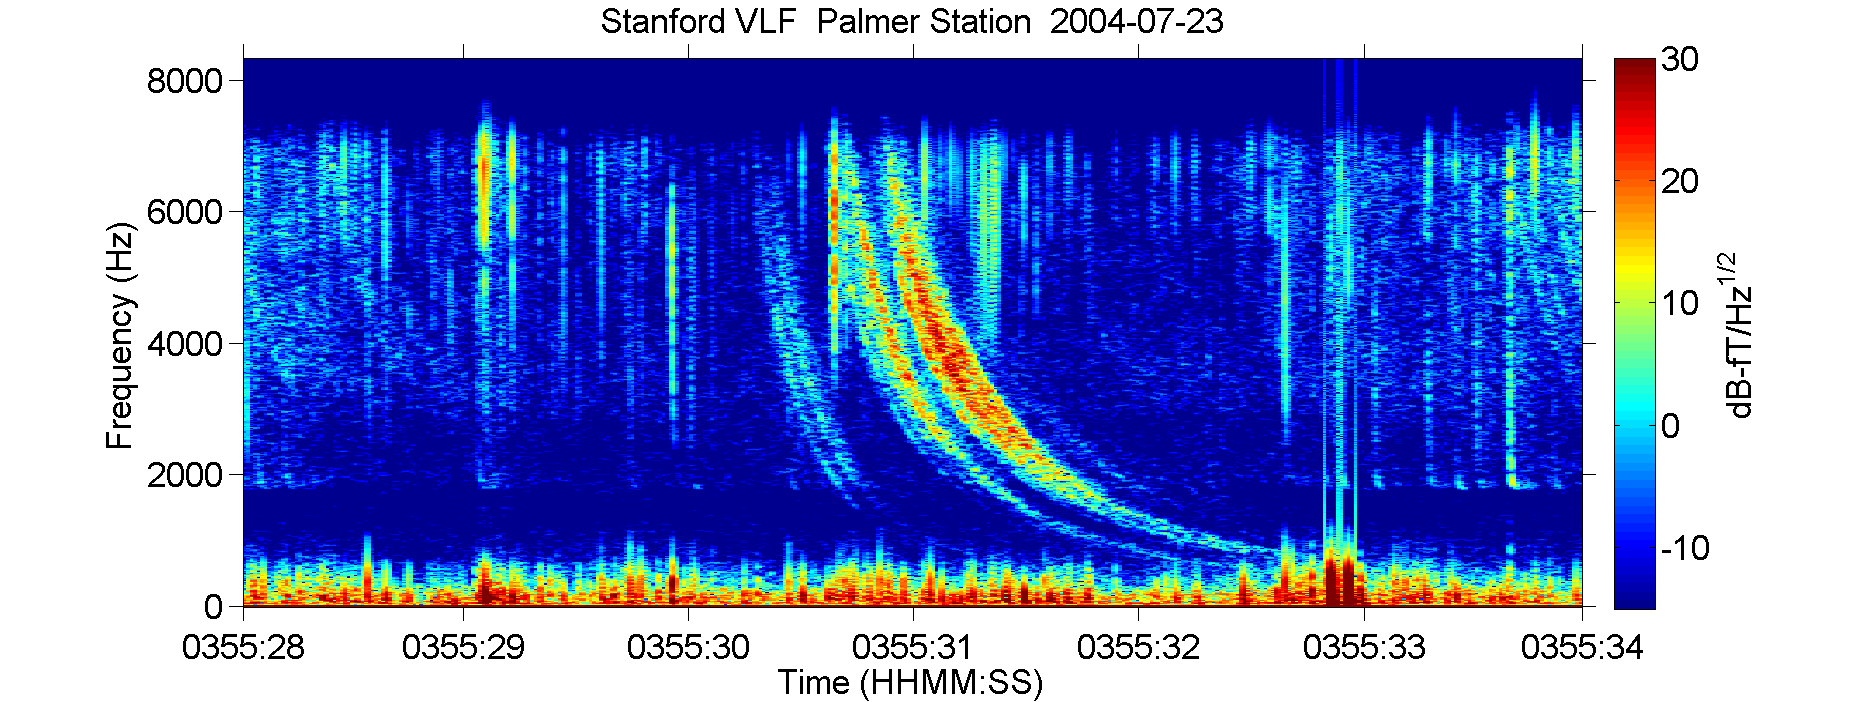
\includegraphics[width=0.95\textwidth]{figures/Whistler_radio_palmer_2004-07-23_T035528.png}

\caption[An example of a lightning-generated whistler wave]{Time-frequency spectrogram of VLF radio wave data from Palmer Station, Antarctica. The short-duration vertical impulses are \emph{sferics}: broadband radio noise radiating directly from a lightning discharge. The curved, sweeping tones result from a fraction of the radio energy propagating out into the plasmasphere, reflecting at the northern hemisphere, and returning to the southern hemisphere. The plasmasphere is a dispersive medium; lower frequencies propagate at a slower velocity than higher frequencies, resulting in the transformation of an impulsive ``click'' into a descending whistling tone. Figure by Dr. Daniel Golden.\footnotemark[2] }
\label{fig:whistlers}
\end{center}
\end{figure}

The concept of lightning as a loss mechanism for radiation belt electrons was first proposed by \cite{Dungey1963}, and subsequently by \cite{Cornwall1964}, through resonant interactions with whistler waves. \citeauthor{Dungey1963} provided order-of-magnitude estimates for electron lifetimes, arguing for the significance of LEP in the inner radiation belt, and against for the outer radiation belt, and proposed an anthropogenic source of whistlers as a provisional loss mechanism in the event of further nuclear enhancements. 

Shortly thereafter, \cite{Kennel1966b}, and subsequently \cite{Lyons1973}, provided an alternative mathematical framework for the diffusion of radiation belt particles due to random-walk interactions with incoherent whistler mode waves known as \emph{plasmaspheric hiss}. From here, studies of wave-induced precipitation mechanisms can be grouped into two categories: coherent studies (the ``Liouville" approach), in which known particles are subjected to a known wave event, and incoherent studies (the ``Fokker-Planck'' approach), in which distributions of particles evolve through repeated, stochastic interactions with broadband radio wave activity.

\footnotetext[2]{Available through Creative Commons at \emph{https://en.wikipedia.org/wiki/Whistler\_(radio)}}

\subsection{LEP measurements}
The first one-to-one measurements of precipitating electrons associated with causative whistlers were presented by \cite{Voss1984}, and subsequently analyzed in \cite{Voss1998}, confirming the feasibility of LEP as a radiation belt loss mechanism. However, due to the sporadic nature of LEP and the dearth of space vehicles to measure it, \emph{in-situ}, one-to-one measurements of LEP remain somewhat rare.
Fortunately LEP can be measured terrestrially across a great distance by examining the perturbations to VLF-band transmitter signals as they propagate in the waveguide formed by the Earth and the charged ionosphere. Additional charges imparted by LEP to the ionosphere can perturb this waveguide, and in turn affect the measured amplitude and phase of transmitted signals. These sporadic events (frequently known as ``Trimpi" events, a nod to their discovery by Mike Trimpi in \cite{Trimpi1973}), have been studied for several decades \citep{Trimpi1973, Carpenter1984, Inan1988, Burgess1993}. These works further confirm the existence and frequency of LEP events; however due to the nature of the waveguide sensing method, it is difficult to obtain direct electron flux estimates without substantial modeling. And even then, evidence for the seasonal variation of LEP is shown in \cite{Gemelos2009}, who present correlations between lightning over the continental United States and particle flux measurements from the DEMETER spacecraft at $\sim$ 600 km.

\subsection{Modeling of single LEP events}
A substantial history of numerical modeling of LEP exists at Stanford, beginning with the thesis work of \cite{Inan1977}, who performed numerical simulations of pitch-angle scattering due to short-duration, monochromatic, ducted whistler waves. This work was then elaborated on throughout the 1980s in a series of test-particle simulations \citep{Inan1982, Chang1983, Chang1983b, Chang1985, Inan1989}, which directly simulate the effect of whistler waves on discrete collections of electrons in the time domain.

Gyrorotation-averaged equations of motion for the interaction of waves and trapped particles were derived by \cite{Bell1984}. Combined with the derivations of \cite{Ristic1992}, the thesis work of \cite{Ristic1993} and subsequently \cite{Ristic1998} provided a mathematical framework for the interaction of generic whistler waves and trapped particles, and demonstrated the relative importance of oblique wave interactions. 

The thesis work and subsequent publications of \citeauthor{Lauben1998} \citep{Lauben1998, Lauben1999, Lauben2001} represented a full numerical treatment of precipitation due to a single lightning stroke, combining test-particle simulations with a numerical raytracing scheme to estimate whistler wave intensity vs. location, frequency and time. The thesis work of \cite{Bortnik2005} brought further detail to the simulation of LEP, again using a raytracing scheme, and incorporating, among other improvements, Landau damping calculations and multiple resonant modes. The work of \citeauthor{Lauben1998} and \citeauthor{Bortnik2005} primarily differ in their treatment of the resonant interaction: \citeauthor{Lauben1998} used a test-particle approach to track the change in particle pitch angles across long distances, while \citeauthor{Bortnik2005} used a hybrid coherent / incoherent scatter model. In this approach, coherent interactions are computed for a collection of particles along a field line with a monochromatic frequency wave, and are then considered independent from other locations and wave frequencies; the resulting resonant interactions are then summed in quadrature across all frequencies and latitudes, to provide a pseudo-coherent, RMS scattering approximation.

The wave-particle interaction model of \cite{Bortnik2005} and \cite{Bortnik2006} was then applied to lightning-driven precipitation through transmitter remote sensing by \cite{Peter2007}, and to narrowband, transmitter-generated waves by \cite{Kulkarni2009} to examine the efficiency of spaceborne VLF transmitters as a remediation tool for radiation belt electrons. \cite{Cotts2011} further expanded on the \citeauthor{Bortnik2005} model by incorporating the effects of atmospheric backscatter.

The work presented in this thesis is based on the original model from \cite{Bortnik2005}; however we provide several model improvements, including an elaborated treatment of the background plasma; a more-accurate model of variation along the longitudinal axis; and various practical code improvements.

% inan 1878, chang + inan thru the 80s, Ristic 1993, Lauben 1998, Bortnik 2005, the ABS stuff, etc
% Should we talk about incoherent methods? They're not really relevant here, but...
\subsection{Behavior of whistler waves in the magnetosphere}
Fully understanding LEP requires study of both the interaction of particles and waves, as well as the behavior of the waves and particles before and after the interaction. The LEP process spans multiple regions of the space environment, and includes physics on timescales ranging from microseconds to minutes. The behavior of whistler waves in the magnetosphere have been studied extensively using the Hamiltonian ray tracing formulation \citep{Stix1992, Landau1975}, beginning with \cite{Haselgrove1955} via a graphical construction technique, and subsequently by \cite{Haselgrove1960} via numerical computation. Over the following decades, the formulation of \citeauthor{Haselgrove1955} was applied extensively to whistler waves \citep{Kimura1966, Edgar1972}, using the `Stanford Ray Tracing Program', a FORTRAN code originally developed by \cite{Walter1969}, with significant improvements by \cite{Inan1977b}, \cite{Ngo1989}, and others. In this thesis we use a modern reworking of the Stanford program, designed by Dr. Forrest Foust in \cite{Golden2010}. Despite a decades-long legacy of work, whistler ray tracing remains an active research pursuit, driven by further improvements to plasmasphere models and increased computational resources. The \citeauthor{Golden2010} model was most-recently expanded by \cite{Maxworth2017} to include warm plasma corrections.

The previously-discussed ray tracing formulations compute wave propagation paths only; a separate treatment is required to compute energy losses due to interactions with the background medium, in a process known as Landau damping. Landau damping was first applied to the whistler mode by \cite{Kennel1966}, and subsequently generalized by \cite{Brinca1972}. While the derivation is detailed, applications of the \citeauthor{Brinca1972} equations are heavily dependent on the temperature profile used \citep{Thorne1994, Bell2002}. Within this work we use a modified temperature profile from \cite{Golden2010}, which combines results from \cite{Bell2002} and \cite{Bortnik2007}.

\subsection{Electron lifetime estimates due to LEP}
LEP is only one of numerous radiation belt loss processes; direct measurements of lifetimes due solely to LEP are difficult to isolate from the combined impact of an equally dynamic and complicated set of source and loss processes. As such, research on the relative contributions of each loss process to the overall timescale of radiation belt lifetimes relies heavily on approximations and models. \cite{Abel1998} divide the VLF spectrum into three separate categories -- hiss, lightning-generated whistlers, and manmade VLF transmitter signals -- and perform a diffusive calculation for each. \citeauthor{Abel1998} conclude that lightning-generated whistlers are an important second-order loss process, but that electron lifetimes are dominantly controlled by plasmaspheric hiss.

Using models of precipitation and a dataset of Trimpi events, \cite{Rodger2003} and subsequently \cite{Rodger2010} estimated the lifetime of radiation belt electrons subject to LEP losses to be on the order of 10 to 100 days, and surmised LEP may be a significant loss mechanism for the inner radiation belt. \cite{Shprits2005} assumed a constant lifetime of $\sim$ 10 days within the plasmasphere, and a faster, empirical fit of $\sim 3$/K$_p$ days outside the plasmasphere, for the combined lifetime of radiation belt electrons subject to all source and loss processes. \cite{Meredith2007}, using wave data from the CRRES spacecraft and the PADIE Fokker-Planck diffusion code, performed a comparative study of ducted whistlers, MR whistlers, and plasmaspheric hiss, for energies between 100 keV and 5 MeV, resulting in widely varying lifetimes between 1 and 10$\E{4}$ days, depending on energy and location. In nearly every scenario considered, \citeauthor{Meredith2007} found the effect of lightning-generated whistlers to be outweighed by hiss. However, the interaction of a short-duration whistler may not be fully captured by a diffusive code, which relies on multiple incoherent interactions to evolve a distribution of particles.
%\cite{barker2005} assumed lifetimes ranging from 6 to 29 days in the outer belt; \cite{Horne2005} determined outer belt lifetimes to be $\sim$ 1 day due to electron microbursts.


%\cite{Shprits2005}, using wave data from the CRRESS spacecraft and a Fokker-Planck diffusion code, estimate electron lifetimes to be on the order of 10 days, dependent on location and solar activity. 

% Abel and Thorne
% Meredeth
% Craig Rodger 2003
% 

\section{Scientific Contribution}
A lack of continuous measurements, both remote and \emph{in-situ}, combined with a wide range of electron energies, the dynamic and sporadic nature of the space environment, and the noise introduced by numerous source and loss processes, has resulted in a lack of consensus on the importance of LEP as a radiation belt loss mechanism. Within this work we seek to quantitatively determine the regions in space and energy where LEP may be of importance, using a combination of raytracing, coherent-interaction modeling, and the introduction of realistic lightning data as measured by the GLD360 lightning detection network. Through modeling, we can examine the impact of LEP independent of the added contributions of numerous other source and loss processes which may overshadow LEP.

The contributions of this work to the scientific community are:
\begin{enumerate}
\item A quantitative estimate of the persistent VLF whistler-mode energy within the plasmasphere and magnetosphere resulting from realistic measurements of terrestrial lightning activity, accounting for variation between day and night, and for variation with K$_p$.

\item Development of a novel interpolation scheme to map unstructured data from a family of rays to their corresponding grid coordinates within the magnetosphere.

\item An improved model of the longitudinal variation of LEP, and an examination of the errors introduced by a two-dimensional approximate scaling function.

\item An examination of the precipitating energy spectrum and total energy deposition below 100 km altitude resulting from LEP, as a function of geographic location, K$_p$, and time of year.

\item Determination of average lifetime estimates for radiation belt electrons subjected to LEP losses, across a wide range of energies (10 eV -- 10 MeV), and L-shells (1.2 -- 7).

\item Development of onboard firmware for a CubeSat-based instrumentation suite, designed for direct, \emph{in situ} measurements of LEP and associated whistlers.
\end{enumerate}
\section{Thesis Organization}
This thesis is divided into the following chapters:
\begin{itemize}
\item Chapter \ref{chapter:physics} describes the background physics of the LEP process, the numerical methods used within this study, and the mathematical models of the different regions of the space environment. 
\item Chapter \ref{chapter:power} presents a study of the persistent VLF radio energy within the magnetosphere, resulting from terrestrial cloud-to-ground lightning discharges as measured by the GLD360 dataset. Variation is explored with respect to geomagnetic longitude and K$_p$. 
%\item Chapter \ref{chapter:3dWIPP} provides a simulation of electron precipitation resulting from a canonical cloud-to-ground lightning discharge, and a discussion of various model improvements, notably with our treatment of the longitudinal axis. 
\item Chapter \ref{chapter:global_estimates} provides a simulation of electron precipitation resulting from single cloud-to-ground lightning discharges, over an array of latitudes, longitudes, and environmental conditions. Using these simulations, we then compute seasonal estimates of the global impact of LEP, driven by the GLD360 dataset. Finally we estimate the average lifetime of radiation belt electrons across a wide range of energies, by simulating electron losses from a uniform population.

\item Chapter \ref{chapter:VPM}, presents the design of a CubeSat-based instrumentation suite, designed for direct, \emph{in-situ} measurements of LEP by taking time-and-space-coincident measurements of electron loss cone distributions, and incident VLF waves. The design provides valueable on-board signal processing to reduce the data bandwidth significantly, and is implemented entirely in fixed-point logic using an FPGA (and \emph{no} onboard CPU). An Air Force Research Laboratory CubeSat based on this design is due to be launched in early 2019.
\end{itemize}



    \chapter[Physics and Methods]{Background Physics and Description of Methods}
        \label{chapter:physics}
    	\section{Overview of Plasma Physics}
A \emph{plasma} is a quasi-neutral gas of ions, electrons, and neutral particles, which exhibit collective behavior. Plasmas can behave in similar ways to a conventional fluid -- they can flow, they can be compressible, they can be turbulent, and so on -- however the addition of charged particles facilitates many behaviors unique to a plasma. Charged particles can interact with each other not just through ballistic collisions, but at a distance through electromagnetic forces. The bulk motion of a plasma can be manipulated through electric and magnetic fields; conversely a plasma can have a substantial effect on the propagation of radio waves passing through it. 

A plasma can be analyzed in several different domains: Single particle motion; fluid approximations; and full kinematic solutions. In this work we treat the motions of electrons in the single particle domain, which is a natural choice for the sparse densities and small gyroradii of radiation belt electrons. To understand the behavior of radio waves propagating through a plasma, we treat the background as a smooth dielectric medium. 

\subsection{Single Particle Motion}
\label{section:single_particle_motion}
The high energies and sparse densities of the radiation belts lend themselves very well to a single-particle approximation. Many of the basic behaviors and quantities in plasma physics can be understood through studying the motion of a single particle.

The fundamental equation of motion for a charged particle in an electromagnetic field is given by the Lorentz force:
\begin{equation}
\vec{F} = \frac{d\vec{p}}{d\emph{t}} = q(\vec{E} + \vec{v}\times\vec{B})
\label{eqn:lorentz_force}
\end{equation}
Where $q$ represents the particle's charge, $\vec{E}$ and $\vec{B}$ represent the electric and magnetic fields, and $\vec{v}$ the particle's velocity, shown here in a non-relativistic frame.

Electric fields simply apply a force in the direction of the field. However, note that a cross product is perpendicular to both terms -- therefore any forces induced by the magnetic field will be perpendicular to the particle's velocity. The magnetic field is a \emph{conservative} force, in that a stationary magnetic field cannot directly impart energy into a particle, but can alter a particle's trajectory. The particle will therefore have a net drift in the direction of the electric field, while exhibiting a helical motion around the magnetic field.

We can then split the velocity vector into two quantities -- $v_\parallel$ parallel to the magnetic field, and $v_\perp$ perpendicular to the magnetic field.

Two characteristic values arise from this motion: the radius of the particle's rotation around the magnetic field, known as the \emph{gyroradius} or the \emph{Larmor radius}:
\begin{equation}
r_l = \frac{m v_\perp}{qB}
\end{equation}

And the rotation frequency, known as the \emph{gyrofrequency} or \emph{cyclotron frequency}:
\begin{equation}
\omega_c = \frac{v_\perp}{r_l} = \frac{q B}{m} \unit{rad/sec}
\end{equation}

By integrating the particle's momentum over a single gyrorotation, we arrive at a third fundamental quantity known as the magnetic moment, or the \emph{first adiabatic invariant}:
\begin{equation}
\mu = \frac{m v_\perp^2}{2B}
\label{eqn:first_adiabatic_invariant}
\end{equation}

In situations where the magnetic field varies slowly (e.g., on spatial scales much greater than the gyroradius), then $\mu$ remains a constant of motion.

A final parameter to describe a particle's motion is it's \emph{pitch angle}, the angle between the velocities perpendicular and parallel to the magnetic field:
\begin{equation}
\alpha = \mathrm{tan}^{-1}\bigg(\frac{v_\perp}{v_\parallel}\bigg)
\end{equation}

The first adiabatic invariant describes an implicit relationship between the magnetic field strength and a particle's pitch angle at a given point. 
Combining the first adiabatic invariant with conservation of kinetic energy, we can deduce an expression for magnetic trapping -- that is, the magnetic field strength in which a particle exhibiting helical motion along a magnetic field line will turn around at. 
\begin{eqnarray}
& E &= \frac{1}{2}mv^2 \\
& &= \frac{1}{2}m(v_\parallel^2 + v_\perp^2) \\
 & &= \frac{1}{2}mv^2(\mathrm{cos}^2\alpha + \mathrm{sin}^2\alpha)
\end{eqnarray}

At a reflection point, the particle's kinetic energy will be entirely in the perpendicular mode:
\begin{eqnarray}
\frac{v_{\perp0}^2}{B_0} = \frac{v_{\perp1}^2}{B_1} \\
\frac{v^2\mathrm{sin}^2(\alpha)}{B_0} = \frac{v^2}{B_1} \\
\mathrm{sin}^2(\alpha)=\frac{B_0}{B_1} 
\end{eqnarray}

Therefore, a charged particle in a magnetic field will be constrained to rotate around a field line, and bounce back and forth, reflecting where the magnetic field strength increases. A key takeaway is that the reflection point is independent of energy, and depends only on the ratio of magnetic field strengths and the particle's initial pitch angle. An example of this behavior is shown in figure \ref{fig:bottle}.
\begin{figure}[ht]
\begin{center}
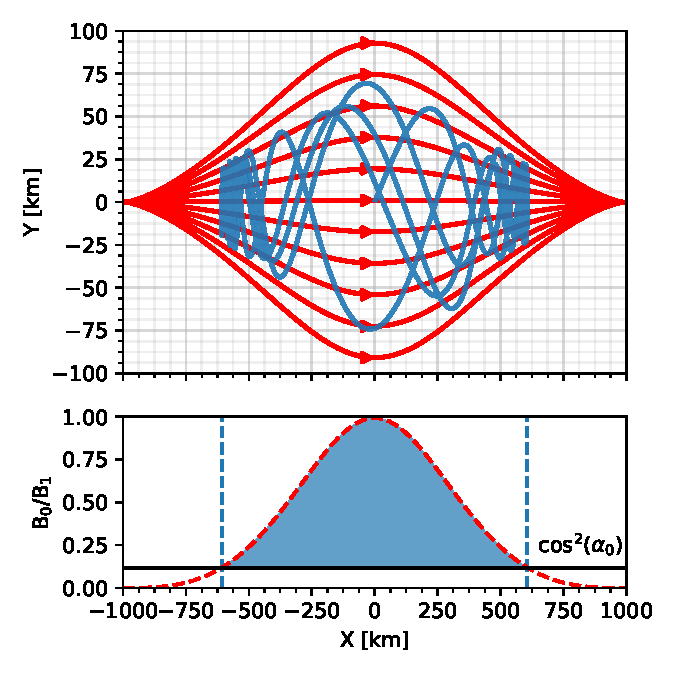
\includegraphics{figures/bottle.pdf}
\caption[An example of a ``magnetic bottle'' particle trap]{An example of a ``magnetic bottle" particle trap. The top plot shows the trajectory of an electron with an initial pitch angle $\alpha_0=20^\circ$. The bottom plot shows the magnetic field ratio $B_0/B_1$, with the particle's reflection points shown as vertical lines. }
\label{fig:bottle}
\end{center}
\end{figure}

\subsection{The Loss Cone}

A magnetic bottle trap need not be linearly-arranged, as it is in figure \ref{fig:bottle}; we require only that the magnetic field be slowly-varying with respect to the particle's gyroradius. The Earth's dipole magnetic field forms a natural and effective particle trap, which dominates the morphology of charged particle populations surrounding the Earth.

The motion of a charged particle in the Earth's magnetic field can be broken into three components: 
\begin{itemize}
\item A rapid gyrorotation around the background magnetic field
\item A ``bouncing'' motion between the north and south poles, with periods ranging from milliseconds to several seconds
\item A slower, longitudinal drift, causing the particles to precess around the earth on the order of minutes to days, resulting from the magnetic field gradient
\end{itemize}

\begin{figure}[ht]
\begin{center}
\includegraphics[draft]{figures/basic_motions.pdf}
% THIS IS THE STANDARD CARTOON OF THE BOUNCE AND DRIFTS...
\caption[Adiabatic motion in the Earth's magnetic field]{Illustration of the various motions exhibited by a charged particle in the Earth's magnetic field}
\label{fig:adiabatic_motions}
\end{center}
\end{figure}

We can average the particle's motion over a single gyrorotation to define a \emph{guiding center}, the trajectory of which follows the background magnetic field line. 

As described previously, a trapped particle's reflection points are defined by the particle's initial pitch angle, and the strength of the magnetic field. In the case of the Earth, however, these turning points are limited in feasibility as well -- for instance, a particle naturally cannot have a reflection point lower than the Earth's surface. Moreover, the Earth's neutral atmosphere becomes exponentially more-dense with decreasing altitude; particles reflecting at an altitude below $\approx 100$ km will encounter a significant neutral molecule population, and stand a very good chance of colliding. A collision with atmospheric constituents can result in the particle losing some, or all, of it's kinetic energy through ionization, and may be completely lost from the system, or return onto a different fieldline \citep{Cotts2011}.

With an understanding of the dense neutral atmosphere, we can define a critical altitude -- 100 km here and in related work -- and thus a critical pitch angle, known as the \emph{loss-cone angle}:
\begin{equation}
\sin \alpha_{lc} = \sqrt{\frac{B(\vec{r})}{B_{h_m}}}
\end{equation}
where $h_m$ is the reflection height, and $B(\vec{r})$ is measured at the reference point -- either the particle's current location for a \emph{local loss cone}, or at the equator along the field line for the \emph{equatorial loss cone}.

\begin{figure}[h]
\begin{center}
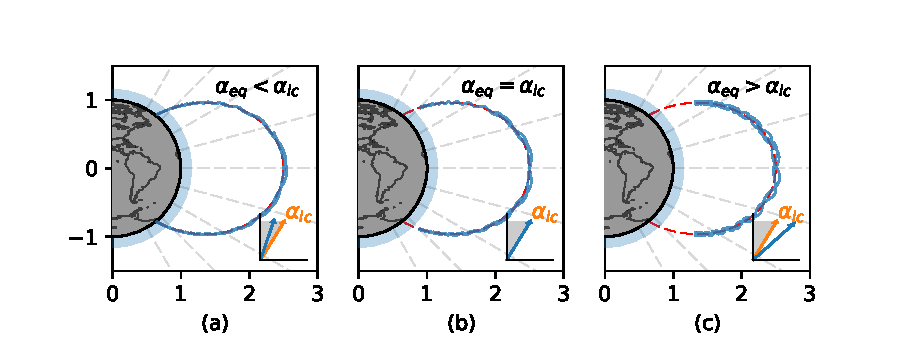
\includegraphics[width=\textwidth]{figures/pitchangle_trapping_3up.pdf}
\caption[Loss cone illustration]{An illustration of the loss cone. The trajectory of a test electron is shown in blue, for three different equatorial pitch angles: (a) a precipitating particle with a pitch angle within the loss cone,  (b) at the edge of the loss cone, and (c), a stably-trapped particle with a pitch angle well outside the loss cone.}
\label{fig:loss_cone_examples}
\end{center}
\end{figure}


In the case of a dipole magnetic field model, we can determine the equatorial loss cone explicitly:
\begin{equation}
\sin \alpha_{lc} = \sqrt{\frac{\zeta_m^3}{\sqrt{1 + 3 (1 - \zeta_m)}}} \qquad \zeta_m = (R_e + h_m) / (L R_e)
\end{equation}
where $R_e = 6371$ km is the radius of the Earth, and L is the \emph{L-shell} of interest (see section \ref{section:dipole_model}).



\paragraph{Bounce and Drift Loss Cones}
We have discussed what is known as the \emph{bounce loss cone}. In literature, there is often mention of both the bounce loss cone and a \emph{drift loss cone}. The drift loss cone is the largest loss cone along the same L-shell, as it varies longitudinally -- conceptually, as a particle drifts longitudinally, it may encounter a different loss cone, and could precipitate at certain longitudes, but not others. 

Under a simple dipole magnetic field model, the two are identical. Within this dissertation, we primarily work with a dipole magnetic field model, and consider only the bounce loss cone.

\subsection{Waves in Plasmas}
Previously, we have described the motion of a charged particle under the influence of an electromagnetic field. the single-particle approximation provides enormous insight into the dynamics of a sparsely-populated plasma. Next, we must consider the inverse system -- how the charged particles in a plasma dictate the characteristic behaviors of an electromagnetic wave propagating through it.

An electromagnetic wave can accelerate a charged particle; conversely, an accelerating or decelerating particle induces its own electromagnetic field. It would seem, then, that the behavior of an electromagnetic field in a plasma is simply the summation of the contributions of each particle and some incident wave source. However, the complexity of this brute-force approach quickly becomes intractable for even a handful of particles. The universal approach taken then is to abstract the complicated interplay of waves and particles into a wave moving through a dielectric medium, described only by the various constituent densities, temperatures, and background field intensities within a given volume. 

As with any electromagnetic problem, we begin with Maxwell's equations -- shown here in their non-relativistic, differential form, in SI units:

\begin{eqnarray}
&\nabla \cdot \vec{E}& = \frac{\rho}{\epsilon_0} \label{eqn:maxwell1}\\
&\nabla \cdot \vec{B}& = 0 \label{eqn:maxwell2}\\
&\nabla \times \vec{E}& = -\frac{\partial \vec{B}}{\partial t} \label{eqn:maxwell3}\\
&\nabla \times \vec{B}& = \mu_0 \vec{J} + \frac{1}{c^2}\frac{\partial \vec{E}}{\partial t} \label{eqn:maxwell4}
\end{eqnarray}

$\vec{E}$ and $\vec{B}$ denote the electric and magnetic fields; $\mu_0$ and $\epsilon_0$ denote the magnetic permeability and electric permittivity of free space; and $c=\sqrt{\frac{1}{\mu_0\epsilon_0}}$ is the speed of light. The terms $\rho$ and $\vec{J}$ represent the local charge density and current density, both of which may be functions of position and time.

By taking the curl of equation \ref{eqn:maxwell3} and substituting in the time derivative of equation \ref{eqn:maxwell4}, and making use of the vector identity $\nabla \times \nabla \times \vec{E} = \nabla(\nabla \cdot \vec{E}) - \nabla^2\vec{E}$, we have:

\begin{equation}
\nabla^2\vec{E} - \frac{\nabla\rho}{\epsilon_0} = \mu_0 \frac{\partial \vec{J}}{\partial t} + \frac{1}{c^2}\frac{\partial^2\vec{E}}{\partial t^2}
\label{eqn:dielectric_tensor_derivation_1}
\end{equation}

In the absence of charges or currents ($\rho=0$, $\partial\vec{J}/\partial t=0$), the equation reduces to the free-space wave equation:
\begin{equation}
\nabla^2\vec{E} = \frac{1}{c^2}\frac{\partial^2\vec{E}}{\partial t^2}
\end{equation}

Next, we linearize the system and search for harmonic perturbations of the form:
\begin{eqnarray}
\vec{E(\vec{r},t)} = \vec{E_1}e^{{i (\omega t - \vec{k}\cdot \vec{r}})} \label{eqn:linear1}\\ 
\vec{B(\vec{r},t)} = \vec{B_0} + \vec{B_1}e^{{i (\omega t - \vec{k}\cdot \vec{r}})} \label{eqn:linear2}\\
\vec{J(\vec{r},t)} = \vec{J_1}e^{{i (\omega t - \vec{k}\cdot \vec{r}})}\label{eqn:linear3} 
\end{eqnarray}

where $\omega$ is the wave angular frequency, $\vec{k}$ is the wave vector, or spatial frequency, and $\vec{r}$ is the spatial coordinate. Two fundamental parameters of an electromagnetic wave are the \emph{phase velocity}, $\omega/k$, and the \emph{group velocity}, $\partial\omega/\partial k$. The relation between the temporal and spatial frequencies is known as the \emph{dispersion relation}.

From here we follow the derivation and convention used by \cite{Stix1992} and \cite{Bittencourt2004}. In general, a plasma is comprised of several different species of constituent particles -- positively and negatively charged particles necessary to maintain a quasi-neutral plasma. While the dispersion relations of different species cannot be simply added, their effects can be summed to form the displacement current $\vec{J}$:
\begin{equation}
\vec{J} = \sum_s\vec{J_s} = \sum_s n_s q_s \vec{u_s}
\label{eqn:J}
\end{equation}
where $n$, $q$, and $\vec{u}$ represent the (number) density, charge, and velocity of a particular species $s$. 

We make the assumption that the plasma is \emph{cold} -- that is, that the velocities of each species $\vec{u_s}$ have a single value each. Were we to relax this assumption, each species density would have a distribution function in both position and momentum, $n=n(\vec{r},\vec{p})$; the total current would then be an integration over momentum for each species. For a treatment of a hot plasma, see the work by \cite{Sazhin1993}.

Next, we note that, in a cold plasma assumption, the Lorentz force (equation \ref{eqn:lorentz_force}) can be written for each species:
\begin{equation}
m_s\frac{d\vec{u_s}}{dt} = q_s\big(\vec{E} + \vec{u_s}\times\vec{B}\big) 
\label{eqn:lorentz_2}
\end{equation}
Combining equations \ref{eqn:linear1} -- \ref{eqn:linear3}, \ref{eqn:J}, and \ref{eqn:lorentz_2}, and assuming a coordinate system with the background magnetic field $\vec{B_0}$ aligned with the z-axis, we arrive at an expression for the \emph{cold-plasma dielectric tensor}:

\begin{equation}
\mvec{\epsilon}\cdot\vec{E}=\begin{pmatrix}
S & -iD & 0 \\
iD & S & 0 \\
0 & 0 & P \end{pmatrix}\begin{pmatrix}E_x \\ E_y \\ E_z\end{pmatrix}
\end{equation}

The various summations over each constituent species are incorporated into the so-called Stix parameters (\cite{Stix1992}):
\begin{eqnarray}
S =\frac{1}{2}(R + L) \qquad D = \frac{1}{2}(R - L)
\label{eqn:stix_params_1}
\end{eqnarray}
\begin{equation}
R = 1 - \sum_s\frac{\omega_{ps}^2}{\omega(\omega + \omega_{cs})}; \quad L = 1 - \sum_s\frac{\omega_{ps}^2}{\omega(\omega - \omega_{cs})}; \quad P = 1 - \sum_s\frac{\omega_{ps}^2}{\omega^2}
\label{eqn:stix_params_2}
\end{equation}

where $\omega_{ps} = n_sq_s^2/{\epsilon_0 m_s}$ and $\omega_{cs}=q_sB_0/m_s$ are the plasma and cyclotron frequencies for species $s$.

\subsubsection{Dispersion Relation}
With the dielectric tensor now determined, we can derive the relationship between $\omega$ and $\vec{k}$, known as the dispersion relation. Equation \ref{eqn:dielectric_tensor_derivation_1} can be written as:
\begin{equation}
\mvec{\eta}\times \mvec{\eta} \times \vec{E} +  \mvec{\epsilon}\cdot\vec{E} = 0
\end{equation}
where $\mvec{\eta} = \vec{k}c/\omega$ is the wave refractive index. Assuming a wave propagating with some angle $\theta$ between $\mvec{\eta}$ and the background magnetic field, we arrive at:
\begin{equation}
\begin{pmatrix}
S - \eta^2\cos^2\theta & -iD & \eta^2\cos{\theta}\sin{\theta} \\
iD & S - \eta^2 & 0 \\
\eta^2\cos{\theta}\sin{\theta} & 0 & P - \eta^2\sin^2{\theta} \end{pmatrix}\begin{pmatrix}E_x \\ E_y \\ E_z\end{pmatrix} = 0
\label{eqn:dispersion_relation_matrix}
\end{equation}

Taking the determinant of \ref{eqn:dispersion_relation_matrix} yields the \emph{cold-plasma dispersion relation}:

\begin{eqnarray}
&A\eta^4 - B\eta^2 + C &= 0 \label{eqn:disp_rln}  \\
&A& = S \sin^2\theta + P\cos^2\theta \\
&B& = RL\sin^2\theta + PS(1 + \cos^2\theta) \\
&C& = PRL
\end{eqnarray}

Equation \ref{eqn:disp_rln} is biquadratic -- we can solve for $\eta^2 = k^2c^2/\omega^2$ using the quadratic formula.

Finally, it is worth noting that when considering a single-species plasma (e.g., electrons only), equation \ref{eqn:disp_rln} reduces to the well-known \emph{Appleton-Hartree Equation} (\cite{Appleton1932}):


\begin{equation}
\eta^2 = 1 - \frac{\frac{\omega_{pe}^2}{\omega^2}}{1 - \frac{\omega_{ce}^2\sin^2\theta}{2(\omega^2 - \omega_{pe}^2)} \pm\big[\big(\frac{\omega_{ce}^2\sin^2\theta}{2(\omega^2 - \omega_{pe}^2)}\big)^2 + \frac{\omega_{ce}^2}{\omega^2}\cos^2\theta\big]^{1/2}}
\end{equation}

%For a simpler derivation of the Appleton-Hartree equation alone, see the classic, approachable text by \cite{Chen1983}.  %% (CHEN DOESN'T SEEM TO DO IT x.x) 

The dispersion relation in equation \ref{eqn:disp_rln} reveals a wealth of information about the characteristics of waves in plasmas. For various plasma densities and background magnetic field strength, we can infer which wave frequencies may propagate, if any, and which wave polarizations. Through the remainder of this work, we will be concerned with the \emph{Whistler} mode -- a right-hand, circularly-polarized (RHCP) wave. Within a typical magnetospheric plasma, the Whistler mode spans the VLF band, roughly between 30 Hz and 300 kHz.

Figure \ref{fig:whistler_mode_dispersion} shows a typical dispersion relation for a magnetospheric plasma (L $\approx$ 2) by plotting frequency vs wavenumber ($\eta = k c/\omega$). The Whistler mode is the lower branch of the RHCP mode.
\begin{figure}[!ht]
\begin{center}
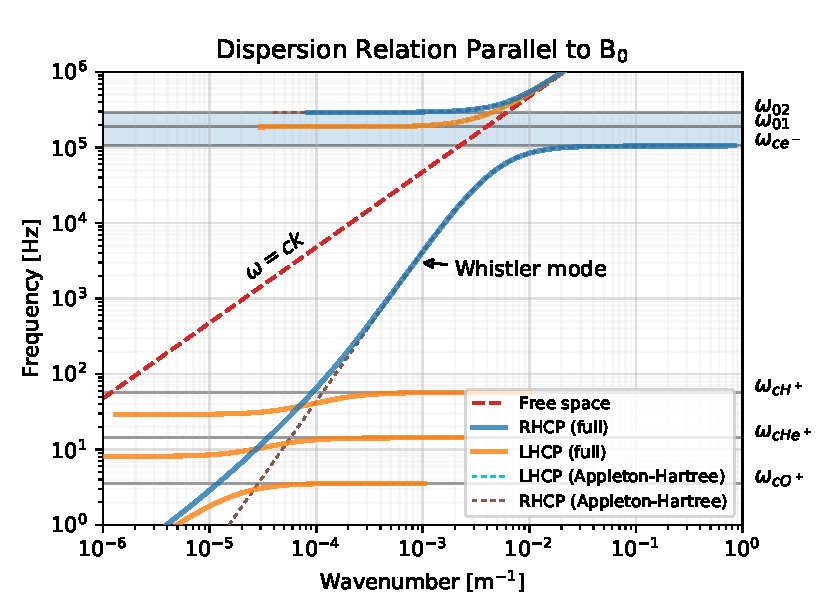
\includegraphics{figures/omega-k_diagram_parallel}
\caption[An $\omega$-K diagram for the cold, four-component dispersion relation, for parallel propagation at L$\approx$3]{An $\omega$-K diagram for the cold plasma dispersion relation, shown here for a wave propagating parallel to $\vec{B}$, in four-component plasma with $N_e \approx  6\E{8}\,e^-/m^3$, and $B\approx 4\,\mu T$. For higher frequencies the dispersion relation asymptotes to the free-space solution, with slope $c$. The Whistler mode is the right-hand, circularly-polarized mode which spans the majority of the frequency band. The shaded region marks the characteristic band in which the right-hand mode cannot propagate. At lower frequencies, the left-hand circular mode resonates with the various ion constituents,  known as the \emph{Ion Cyclotron} modes.}
\label{fig:whistler_mode_dispersion}
\end{center}
\end{figure}

\section{Ray Tracing and Landau Damping}
\label{section:raytracing}
\subsection{Ray Tracing}
Whistler-mode waves in the magnetosphere propagate for very large distances, and with relatively little attenuation. Under certain conditions, these waves can persist from a few seconds to 1 or more minutes. Simulating the propagation of these waves using a full-wave method would be extremely intractable with current computational resources. However we can use ray tracing to approximate their behavior.

Ray tracing is a technique from geometric optics which tracks the position and velocity of a coherent wave packet -- essentially, approximate the behavior of a wave packet to that of a photon, and evaluate the packet's velocity and wavenormal vector with respect to time. Ray tracing is best suited for coherent, monochromatic wave packets, with no attenuation, dispersion, or mode coupling. 

Ray tracing was first applied to the Whistler mode by \cite{Haselgrove1955} using a graphical technique, then subsequently by \cite{Haselgrove1960} and \cite{Kimura1966} for numerical computation. These papers worked in curvilinear coordinates with respect to a magnetic field line. Haselgrove's Equations have been used extensively by numerous magnetospheric scientists \citep{Kimura1966, Edgar1972, Ngo1989,Ristic1993, Lauben1998, B.Peter2007, Bortnik2005, Kulkarni2009}, several using the so-called ``Stanford Ray Tracing Program'' -- a legacy Fortran code which evaluated the Haselgrove equations in two dimensions. Our work uses a slightly different code originally developed by Dr. Forrest Foust \citep{Golden2010}, and is designed for flexibility with respect to plasma density and magnetic field models. Rather than work in curvilinear coordinates with explicit derivatives, we adopt a more-general formulation, using a three-dimensional Cartesian frame and numerically-evaluated derivatives.

We begin with the fundamental ray-tracing equations, as given by \cite{Haselgrove1960, Stix1992}:

\begin{eqnarray}
\frac{d\vec{r}}{dt} = \frac{\nabla_kF}{\partial F/\partial \omega} \label{eqn:raytracing_position}\\
\frac{d\vec{k}}{dt} = \frac{\nabla_rF}{\partial F/\partial \omega} \label{eqn:raytracing_wavenormal} \\
\end{eqnarray}
Constrained such that:
\begin{equation}
F = F(\vec{r},t,\vec{k},\omega) = 0
\end{equation}
Equation \ref{eqn:raytracing_position} is simply $\frac{\nabla_kF}{\partial F/\partial \omega} \approx\frac{\partial F/\partial k}{\partial F /\partial \omega} = \frac{\partial \omega}{\partial k} = v_g$, the group velocity of a wave packet. The corresponding equation describing the evolution of the wavenormal vector (\ref{eqn:raytracing_wavenormal}) is less intuitive, although an analogy can be drawn to Hamiltonian mechanics, in which $\omega$ represents a velocity, and $k$ a momentum.

The function F, our ``conserved quantity'', is simply the cold plasma dispersion relation given by equation \ref{eqn:disp_rln}.

The raytracing equations are a set of coupled, first-order differential equations; solutions to which require some subtlety, but can be addressed using standard numerical techniques.

First, note that we can solve the set at a given time, then evolve the system forward some finite time step. However, the constraint $F=0$ may not be strictly held afterward. We assert that the error in this constraint must be small; which in turn implies that the background medium must be smoothly-varying -- i.e., changing on a spatial scale much greater than our forward step, and of the wavelength of interest. This assumption is known as the \emph{WKB Approximation}.
\begin{figure}[ht]
\begin{center}
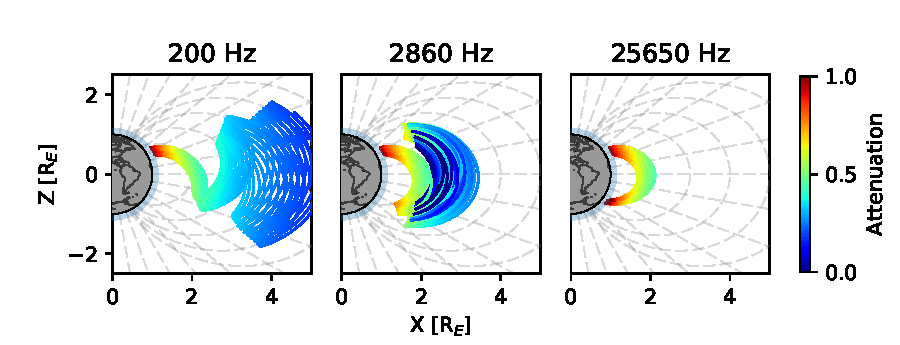
\includegraphics{Figures/raytracing_example.pdf}
\end{center}
\caption[Example ray tracing]{Example ray families as computed by the raytracer}
\end{figure}
\subsubsection{Adaptive Timestepping}
The process of raytracing, then, is to 1) solve the dispersion relation (\ref{eqn:disp_rln}) to find the refractive index; 2) compute the velocity vector and step the system forward in time; and 3) re-evaluate at the new position to assure that the condition F=0 is satisfied. However, properly selecting the timestep is of critical importance -- too large a timestep and positional errors will accumulate, or the ray will slip out of a propagating mode; too small and computational speed and memory usage suffers. We use an adaptive \emph{Runge-Kutta-Fehlberg} (RK45) \citep{Fehlberg1969, Mathews2004} method to continuously update the timestep as the raytracer progresses. RK45 is a common technique for solving ordinary differential equations.

The RK45 method approximates a solution with an initial stepsize $dt$ using two spline fits: a fourth-order and a fifth-order. The error in the step is taken to be the difference between the two estimates. If the error is above a specified tolerance $\epsilon$, the stepsize is reduced and the evaluation is repeated. Additionally, if the error is below a specified tolerance ($\epsilon/10$ in our implementation), the stepsize is increased. The result is a variable time axis with finer resolution in regions of high variability, while enabling longer timesteps in smooth regions for computational efficiency. See appendix \ref{appendix:runge_kutta} for a detailed description of the Runge-Kutta method.

\subsection{Landau Damping}
\label{section:damping}
The cold-plasma formulation of raytracing described above evaluates the trajectory and wavenormal angle of a wave packet. However, it assumes zero attenuation of wave energy. While it is possible to account for wave attenuation in ray tracing using warm plasma corrections \citep{Sazhin1993, Henyey1980}, we follow the same approximation as used in the legacy ray tracing code, and calculate attenuation along the cold-plasma raypath according to Landau damping.

Landau damping, originating in a seminal work by \cite{Landau1946}, is a resonant interaction between a wave and the distribution of electrons and ions comprising the background medium. The Landau mechanism is an interaction with parallel streaming particles and the wave's electric field. Resonant particles are accelerated or decelerated by the wave's electric field; if a majority of the resonant electrons have velocities slightly below that of the wave, then a coherent effect exists, the wavefront imparts some net energy to the plasma, and the wave is attenuated. Conversely, if the majority of resonant particles are moving faster than the wave, some of their energy can be imparted to the wavefront, inducing \emph{wave growth} \citep{Chen1983, Kulkarni2009}. 

Landau damping can have multiple resonances (in which the particle has multiple complete rotations per rotation of the wave). The lowest resonant mode is known as the \emph{Landau} resonance, while the $\pm 1$ modes are referred to as the \emph{Cyclotron} resonances. Higher-order modes remain nameless.

We use the expressions for Landau damping as formulated by \cite{Brinca1972}. \citeauthor{Brinca1972} derived expressions for Landau damping assuming a cold background plasma with a sparse warm distribution added, for Whistler waves propagating at an arbitrary angle to the background magnetic field. Inputs to this formulation are the familiar Stix parameters (equations \ref{eqn:stix_params_1} - \ref{eqn:stix_params_2}), which are in turn a function only of location and wave frequency; the wavenormal angle with respect to the background magnetic field; and a distribution function which specifies the energies (and thus velocities) of thermal electrons. The full set of Landau damping equations is given in appendix \ref{appendix:landau}.

Interestingly, \citeauthor{Brinca1972}'s work was motivated by measurements of Whistler-mode wave growth, rather than attenuation. Our implementation follows suit, and is equally capable of returning growth or damping, depending on the plasma model used. However, throughout this research, wave growth has been exceedingly rare.

\subsubsection{Thermal electron distributions}
\label{section:thermal_electron_distributions}
The extent to which a wave is amplified or damped is heavily dependent on the energy distribution of background electrons. The energy distribution, or temperature profile, is specified as a normalized function in phase space -- a function of position and velocity, which is normalized to 1:

\begin{eqnarray}
f  & = & f(\vec{r}, \vec{v}, t) \\
& =  & f(\vec{r}, v_\perp, v_\parallel, t) \\
\int_0^\infty f d v_\perp & = & 1 \\
\end{eqnarray}

Two distribution functions are used in similar work -- the \cite{Bell2002} distribution, which was derived from POLAR spacecraft measurements of the inner plasmasphere, and the \cite{Bortnik2007} distribution, which is based on CRRES spacecraft measurements above L $\approx$ 7.

We use the phase space density function as described in \cite{Golden2010}, which smoothly transitions between the \cite{Bell2002} model inside the plasmapause, and the \cite{Bortnik2007} model outside the plasmapause. Figure \ref{fig:phase_space_density} shows an example of the distribution function.

\begin{figure}[ht]
\begin{center}
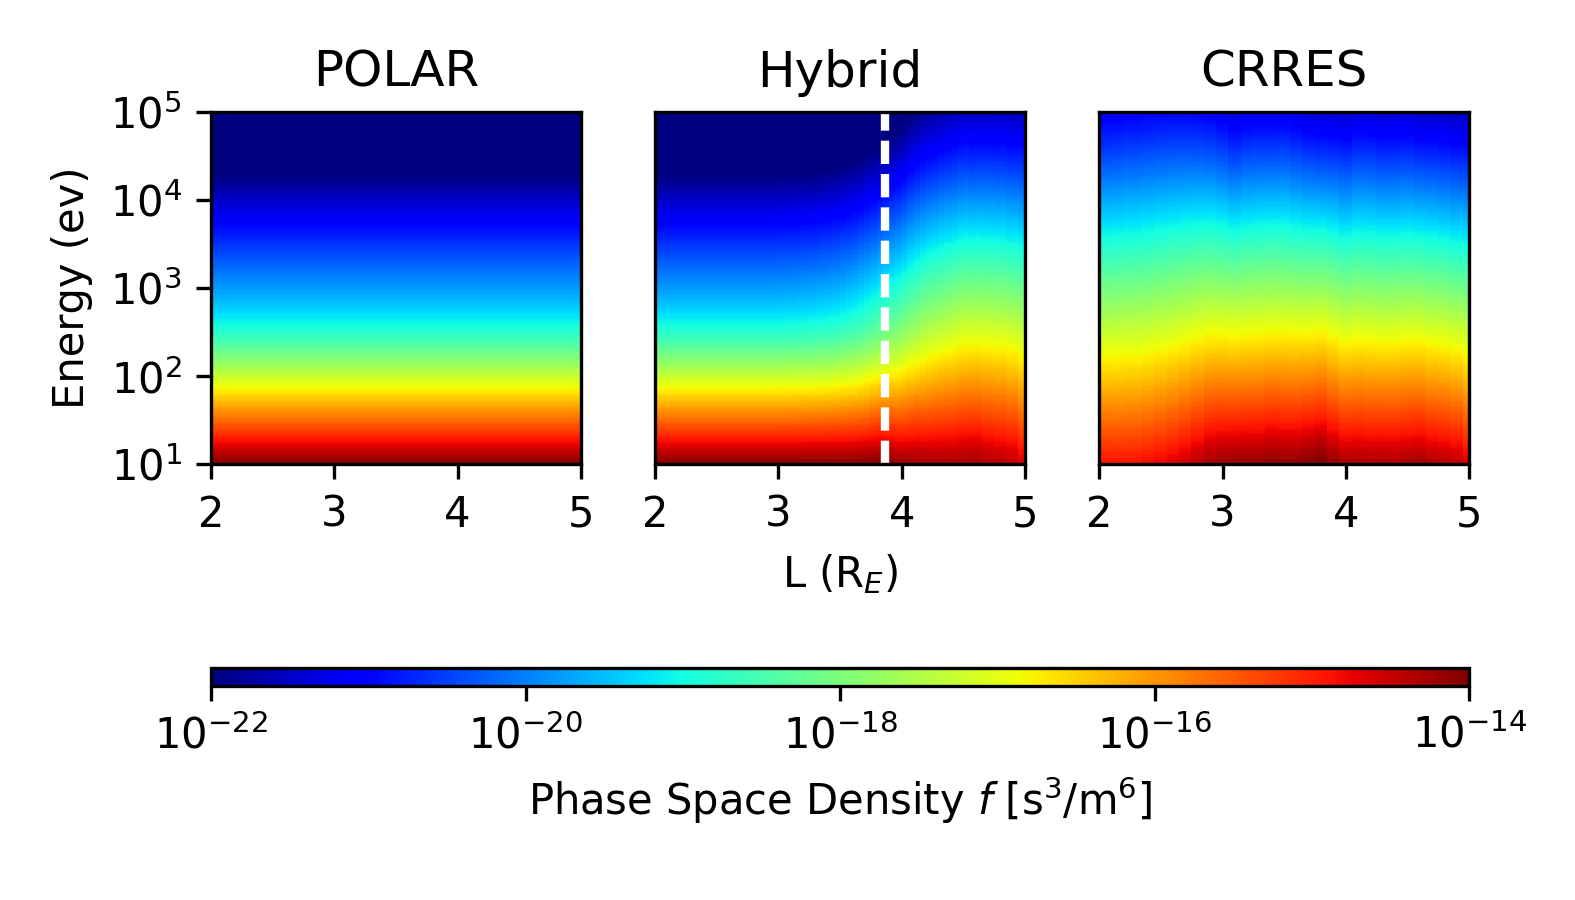
\includegraphics{Figures/psd.png}
\end{center}
\caption[Phase-space density functions]{Example phase-space density functions, shown for $A_e$=1.6, $K_p$=4, $\alpha$=45$^\circ$, and MLT=18. The POLAR model is used inside the plasmapause, and the CRRES model outside the plasmapause. The hybrid model smoothly transitions between the two. The plasmapause, at $L\approx 4$, is marked by the dashed white line.}
\label{fig:phase_space_density}
\end{figure}









\section{Coordinate Systems}
In dealing with any geographic system, one will almost surely run into difficulty with coordinate systems. Most research fields make use of different coordinate systems which better-suit the minutia of their work. Since LEP is a large-scale coupling process which spans several different regions of the Earth and Space Environment, it is useful to discuss the coordinate systems we will use, and the processes of mapping from frame to frame. For an in-depth review of many additional coordinate systems, see the work by \cite{Laundal2016}.

\paragraph{Geographic and Geodetic coordinates}

\paragraph{Magnetic Dipole coordinates}

\paragraph{Earth Centered, Earth Fixed (ECEF)} 

\paragraph{Solar Magnetic}

\paragraph{Mapping vector quantities between polar and Cartesian frames}


\section{Lightning Illumination Model}
\label{section:input_power}
%\subsection{Emission Spectrum}
A single lightning flash is a stochastic dielectric breakdown process. While a terrestrial lightning flash consists of several repeated strokes at varying incident angles, we adopt the simplified model used by \citealt{Lauben1998}, \citealt{Bortnik2005}, and subsequent workers, and encapsulate the entire discharge process in a single return stroke.

The lightning flash is modeled as a single, vertical current pulse from a height $H_E$, with a double-exponential time profile given by equation \ref{eqn:td_pulse}. The double-exponential current profile is simple and common in the literature, originating with \cite{Bruce_Golde_1941}:
\begin{equation}
\label{eqn:td_pulse}
I(t)=I_0(e^{-a t} - e^{-b t})
\end{equation}

We relate the time-domain current profile to radiated power using the far-field approximation for an arbitrary source, given by \cite{Griffiths1999}, page 457:
\begin{equation}
\label{eqn:griffiths_power}
S(t) \approx \frac{1}{\mu_0}(\mathbf{E} \times \mathbf{B}) = \frac{\mu_0}{16\pi^2c}\left[\ddot{p}(t)\right]^2 \left(\frac{\sin^2\theta}{r^2}\right)\mathbf{\hat{r}}
\end{equation}

where $p(t)$ is the dipole moment given by $p=2 H_E \int_0^t{I(t)}dt$, r is the distance from the flash in meters, and $\theta$ is the angle to the flash. Taking the second derivative of the dipole moment (the first derivative of the current profile) gives us the far-field time-domain power equation:

\begin{equation}
\label{eqn:farfield_power_td}
S(t) = \frac{1}{Z_0}\left(\frac{\mu_0 H_E I_0}{2 \pi}\right)^2\left(\frac{\sin^2\theta}{r^2}\right) \left(a e^{-a t} - b e^{-b t}\right)^2  \mathbf{\hat{r}}
\end{equation}

where we have used the relation $Z_0 = \mu_0 c$. Equation \ref{eqn:farfield_power_td} has units of energy flux density, Watts per square meter ($J/m^2/$sec).

To determine the frequency spectrum of the radiated power, we take the Fourier transform of equation \ref{eqn:farfield_power_td}:

\begin{equation}
\label{eqn:farfield_power_fd}
S(\omega) = \frac{1}{Z_0}\left(\frac{\mu_0 H_E I_0}{2 \pi}\right)^2\left(\frac{\sin^2\theta}{r^2}\right) \frac{\omega^2(a-b)^2}{\pi(\omega^2 + a^2)(\omega^2 + b^2)}  \mathbf{\hat{r}}
\end{equation}

which has units of energy flux per frequency -- J/m$^2$/Hz.

Throughout this work we assume a flash height $H_E$=5 km, and model parameters $a=5\E{3}\,\mathrm{sec}^{-1}$ and $b=1\E{5}\,\mathrm{sec}^{-1}$, resulting in a spectrum peaked at approximately 4kHz; any lightning flash can be parameterized solely by its peak current $I_0$ and its location on the surface of the Earth. Figure \ref{fig:lightning_spectrum} shows the current profile and associated spectrum.

The total energy released in a single discharge is determined by integrating equation \ref{eqn:farfield_power_td} over time and a half-sphere surface:

\begin{eqnarray}
\label{eqn:total_energy_below_iono}
E &= &\int_{t=0}^\infty \int_{\phi=0}^{2\pi} \int_{\theta=0}^\pi  S(t) r^2 \sin\theta\,d\theta\,d\phi\,dt \\
 & = & \frac{1}{Z_0}\bigg(\frac{\mu_0}{2\pi}\bigg)^2 \, \frac{(a - b)^2}{2 (a + b)}  \, \frac{4 \pi}{3} \, H_e^2 I_0^2 \\
 & \approx & 1.9\E{-14}H_e^2 I_0^2 \unit{Joules}
\end{eqnarray}


\begin{figure*}
\begin{center}
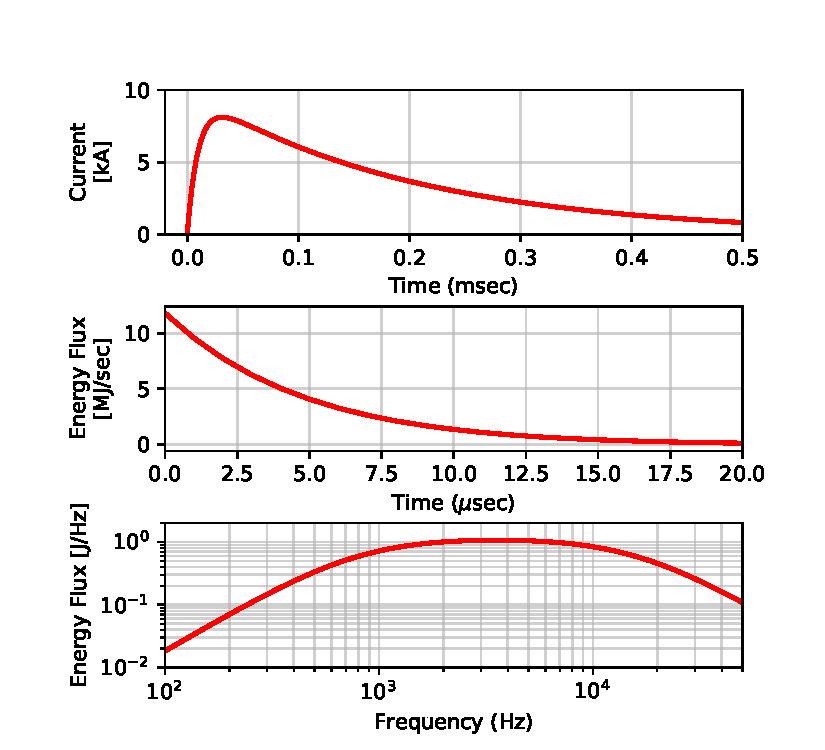
\includegraphics{figures/Lightning_spectra.pdf}

\caption[Time and frequency profiles of the lightning illumination model]{Double-exponential current pulse model of a lightning stroke. The top panel shows the stroke current vs time; the middle panel shows the total energy flux, integrated over space, vs time; the bottom panel shows the energy flux in the frequency domain.}
\label{fig:lightning_spectrum}
\end{center}
\end{figure*}


\section{The Ionosphere}
The ionosphere, extending from $\approx$ 85 km to 1000 km, is the highly-variable transition region between the terrestrial neutral atmosphere and the sparse plasmas of the space environment. The relatively-sharp rise in electron density at the bottom of the ionosphere makes it highly-reflective within the VLF band, forming a waveguide between it and the conductive surface of the Earth. However, In studying LEP, we are primarily concerned with the fraction of energy which does not reflect, and instead propagates through the ionosphere and out into the plasmasphere.

\subsection{Trans-Ionosphere Attenuation}
\label{section:trans_ionosphere_atten}
The ionosphere is a region of high variability, and a significant factor in the LEP process. As discussed earlier, the majority of VLF energy emitted by a lightning flash propagates efficiently in the Earth-Ionosphere waveguide; however a fraction of emitted energy can propagate upwards through the ionosphere, where the wave experiences significant losses via Joule heating in the D-region ionosphere \citep{Graf2013, Marshall2014, Blaes2016}.

Propagation through the ionosphere can be studied using a raytracing approach; however the techniques required differ substantially from the raytracing implementation used in section \ref{section:raytracing}. First, a key assumption in raytracing is that the background medium is smoothly-varying over each timestep (known as the WKB approximation, in reference to the three researchers Wentzel, Kramers, and Brillouin, who independently developed the technique in 1926 \citep{Bender1999}). Maintaining this assumption requires different time steps and error bounds than within the plasmasphere, and would need to be computed separately. Second, the Landau calculations used to compute ray damping are designed for warm, but collisionless plasmas; the ionosphere is collisional, and only partially ionized, requiring different treatment.

Ionospheric propagation is further complicated by reflection and transmission at the lower boundary layer, as well as mode-coupling between incident plane waves, the whistler mode, and various others. 

For computational simplicity, and to more-easily generalize to a variety of conditions, we treat the ionosphere as a single absorbing slab, ranging from 100 to 1000 km in altitude. We assume that waves propagate directly upwards (normal to the Earth's surface), and are not deflected by ionospheric irregularities or the inclination of the background magnetic field.

Numerous researchers \citep{Lauben1998, Bortnik2005, Kulkarni2009, Graf2013} have used the classic ``Helliwell" curves, taken from \cite{Helliwell1965}, Figure 3-35. Helliwell performs an analysis similar to Landau damping -- first deriving a dispersion relation for a collisional plasma, then separating out the imaginary component, which will result in a real-valued attenuation term. The resulting attenuation term is dependent on electron density as a function of altitude, which was extrapolated from sounding rocket campaigns for day and night. The net attenuation is then computed by integrating from 65 to 1500 km in altitude.

Helliwell's curves have persisted as the default record of trans-ionospheric attenuation; however it has been shown that Helliwell's curves overestimate trans-ionosphere attenuation by 10 to 20 dB \citep{Starks2008}, due mainly to the coarse measurement of the ionosphere electron density profile.

Rather than Helliwell's curves, we use results from \cite{Graf2013}, which are derived from extensive full-wave simulations using the International Reference Ionosphere (IRI) plasma density profile. Related work using the same full-wave model has been experimentally verified at $\sim$20 kHz using DEMETER satellite measurements of VLF transmitters \citep{Cohen2012}. \citeauthor{Graf2013} reports a set of curves in the same manner as Helliwell -- power attenuation as a function of latitude, for two frequencies (2 kHz and 20 kHz), for dayside and nightside ionospheres. We then interpolate (or extrapolate) in log-space to find an attenuation factor for any latitude or frequency of interest ($\approx 10^\circ - 70^\circ$, and 200 Hz - 30 kHz).

We transition between the dayside and nightside attenuation curves using a Sigmoid function, with an approximate 1-hour transition width.

Figure \ref{fig:graf_curves} compares the \cite{Graf2013} and \cite{Helliwell1965} attenuation curves, which model the integrated wave power losses between 65 km - 1500 km altitude as a function of frequency and geomagnetic latitude. Both models exhibit similar trends -- higher attenuation towards the equator, and higher attenuation on the dayside -- however the Helliwell curves report significantly greater attenuation overall. We can attribute this due to the electron density profile used in their calculation.

% (Also here's where you left off in incorporating Bob's edits, 1.12.2018)

\begin{figure}[h]
\begin{center}
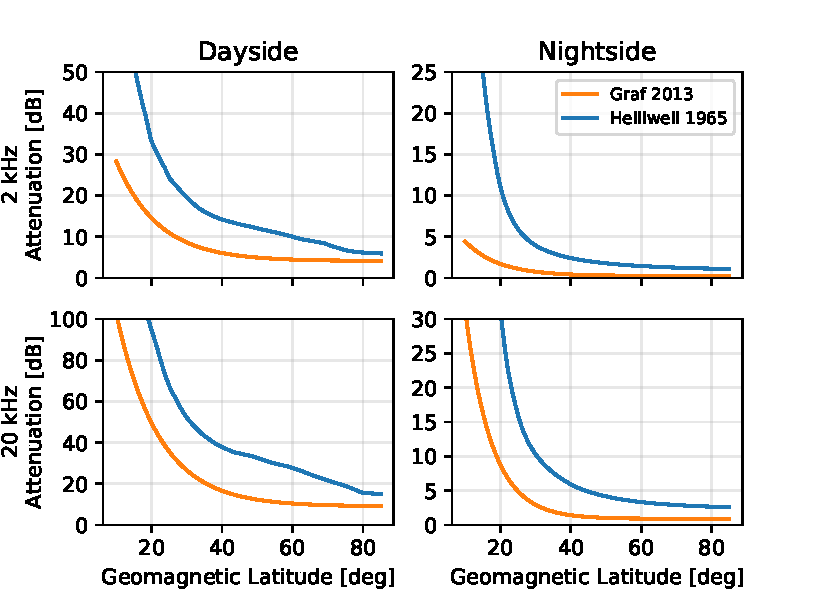
\includegraphics{figures/iono_absorp_curves}
\caption[Trans-Ionosphere attenuation curves for day and night]{Trans-Ionosphere attenuation curves for the dayside and nightside, at 2 kHz and 20 kHz. Reproduced from \cite{Graf2013}, figure 7. The \citeauthor{Graf2013} curves show markedly less attenuation than the previously-used \citeauthor{Helliwell1965} curves, especially at equatorial latitudes, and on the day side.}
\label{fig:graf_curves}
\end{center}
\end{figure}


\subsection{Models of the Ionosphere}
In general, our treatment of wave propagation in the ionosphere is abstracted using the method described in Section \ref{section:trans_ionosphere_atten}. However, in raytracing through the plasmasphere, we require a smoothly-varying transition between the plasmasphere and ionosphere models. Here we discuss two models of ionosphere electron density.

\paragraph{IRI:}
The International Reference Ionosphere (IRI) is a standard model of several key plasma parameters -- electron density, electron and ion temperatures, ion composition, and so forth. IRI provides detailed outputs as a function of location, altitude, and local time. The GCPM plasma model (a comprehensive model of the plasmasphere, described in section \ref{section:gcpm}) uses the IRI-2007 implementation \citep{Bilitza2008}; the simplified IRI model is derived from the IRI-2016 model (the most-current available version at time of writing).

\paragraph{Simplified IRI:}
\begin{figure}[h]
\begin{center}
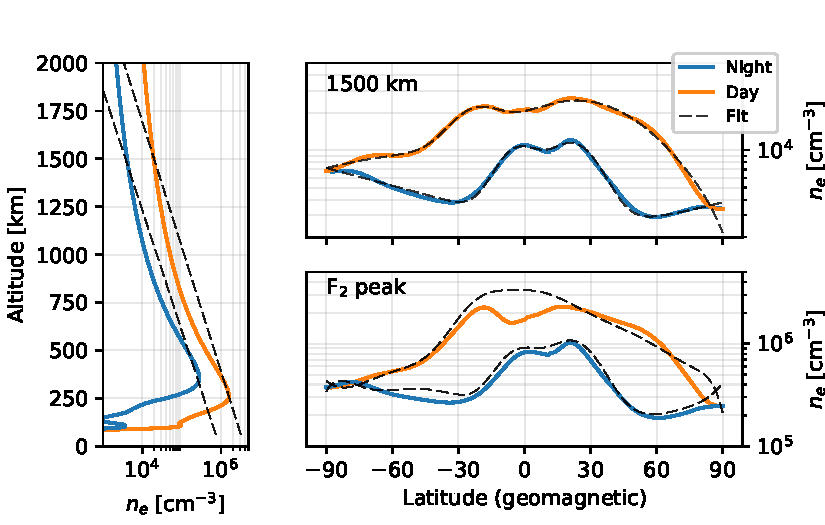
\includegraphics{figures/iono_profile.pdf}
\caption[Ionosphere density profile]{The IRI electron density model and derived curve fits. The left panel shows electron density variation as a function of altitude, for day and night. The right panels show electron density variation with respect to latitude, for (top) 1500 km and (bottom) the $F_2$ peak (approx. 300 km). Dashed lines indicate the fitted curves used by the simplified IRI model.}
\label{fig:iono_profile}
\end{center}
\end{figure}

In order to both reduce our model parameter space, and to greatly decrease computation time, we pair a simplified version of IRI with a simplified version of GCPM. The IRI-2016 model was run for dayside and nightside ionospheres (12 and 0 MLT), using all default settings, for January 1st, 2000. We then fit a multiple-Gaussian function to the electron density vs latitude, at an altitude of 1500 km, and at the $F_2$ peak. Electron density variation with respect to altitude is approximated by a log-linear fit between 1500 km and the $F_2$ peak. Finally, longitudinal variation is smoothed with a sigmoid function with a width of $\sim$ 1 hr. Figure \ref{fig:iono_profile} shows both the IRI electron density and the derived curve fits.



\section{Wave-Particle Interactions}
%\section{Environment Models}
%Within this work, we will encounter several different regions of the space environment -- This section provides a collected overview of each region and the models used.
%\subsection{Magnetic Field}
%\paragraph{Magnetic Dipole}
%\label{section:dipole_model}
%To first order, the Earth's magnetic field can be approximated as a dipole, with origin at the Earth's center, and a tilt of $\approx 11^\circ$ from the axis of rotation. The dipole model, sometimes referred to as the ``centered dipole'' or ``tilted dipole'', is reasonably accurate for midlatitude field measurements over the continental United States, but can deviate significantly from the true field elsewhere. Similarly, the dipole field model is reasonably accurate for middle latitudes, below $\approx$ 10 Earth radii, but become increasingly inaccurate at higher latitudes, and at larger distances from the Earth, where the Earth's internal field is no longer dominant.
%
%The dipole model, however, excels in its simplicity -- the dipole magnetic field can be completely described in a closed form, and can be computed rapidly and reliably.
%
%The dipole potential is given by:
%\begin{equation}
%\psi_{dip} = B_0\big(\frac{R_e}{r}\big)^2\cos\theta
%\end{equation}
%
%The individual components of the magnetic field are given by the negative gradient of the scalar potential:
%
%\begin{eqnarray}
%& \vec{B} = -\nabla \psi \\
%& B_r = -2 B_0\big(\frac{R_e}{r}\big)^3\cos\theta \\
%& B_{\theta} = -B_0\big(\frac{R_e}{r}\big)^3 \sin\theta \\ 
%& B_\phi = 0
%\end{eqnarray}
%
%Within this work we use $B_0 = 31.5$ $\mu$T and $R_e=6371$ km.
%
%A single fieldline, determined by integrating the direction of the field vector, can be described by it's \emph{L-shell} -- the fieldline's altitude, in units of Earth radii, measured at the equator. 
%
%For the dipole field, the radius of a field line at any latitude is related by:
%\begin{equation}
%R(\lambda) = R_e L \cos^2 \lambda
%\end{equation}
%
%
%The dipole field can then be used as an orthogonal coordinate system, with any location being specified by a latitude, longitude, and L-shell \citep{McIlwain1961}. 
%
%Within the plasmasphere, the dipole model works well. However, closer to the Earth's surface the model becomes increasingly inaccurate, necessitating a higher-order model.
%\paragraph{IGRF}
%The International Geomagnetic Reference Field (IGRF) is a 13th-order spherical expansion model, with coefficients updated every few years based on terrestrial measurements \citep{Thebault2015}. Within this work we use the IGRF-12 model as a realistic representation of the Earth's internal magnetic field.
%
%IGRF is quick and simple to calculate at any given location, and is much closer to reality than a simple dipole field. However, due to the added complexity, there are not closed-form expressions for field line trajectories or L-shells, which can make dealing with IGRF (and any higher-order model) more cumbersome.
%
%Figure \ref{fig:Lshell_example} contrasts lines of constant L-shell between the dipole and IGRF models.
%
%\paragraph{Tsyganenko Corrections}
%The dipole and IGRF models represent the Earth's internally-generated magnetic field. However, as one moves further away from the Earth ($L > \sim 8$), the Earth's internal field becomes less dominant, and external fields, namely forcing from the solar wind, cannot be ignored. The total field present in the space environment is the sum of both internal and external contributions.
%
%Numerous models of the external field exist; within this work we consider the T05 external field model \citep{Tsyganenko2005}. The external field model exhibits seasonal and daily variation. However, for fieldlines below L $\approx$ 6, the external field effects can be ignored. 
%
%Figure \ref{fig:fieldline_example} contrasts the dipole, IGRF, and T05-corrected models in the meridional plane; Figure \ref{fig:Lshell_example} illustrates the deviation in fieldline contours along the Earth's surface between the dipole and IGRF models.
%
%\begin{figure}[h]
%\begin{center}
%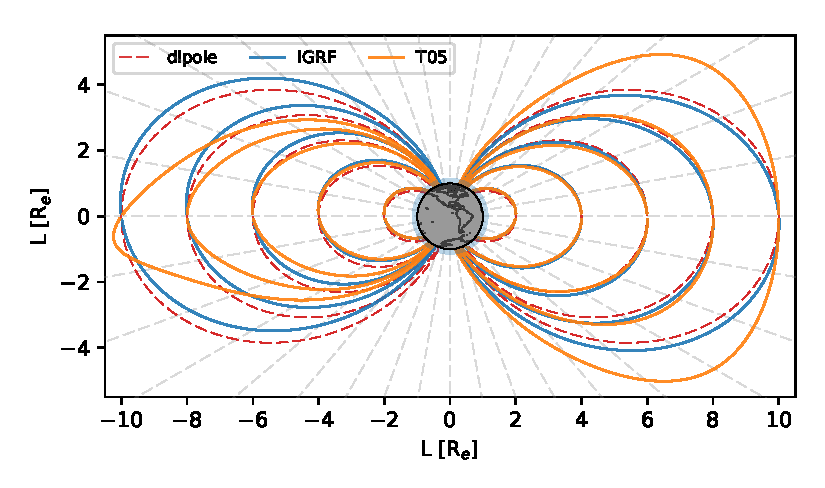
\includegraphics{figures/fieldline_models.pdf}
%\end{center}
%
%\caption[Magnetic field models]{Three different magnetic field models, shown in the meridional plane, in geomagnetic coordinates: the tilted dipole, the IGRF model, and the Tsyganenko-Corrected IGRF model. Solar wind is incident on the right side.}
%\label{fig:fieldline_example}
%\end{figure}
%\begin{figure}[h]
%\begin{center}
%	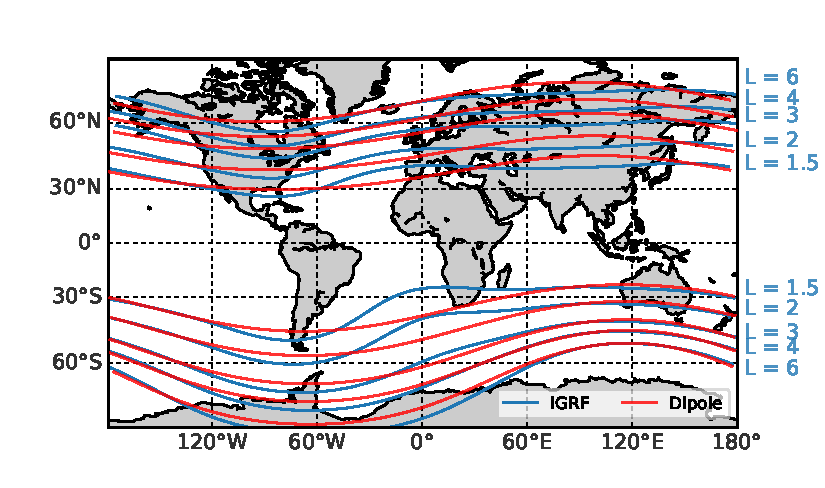
\includegraphics{figures/Lshell_contours.pdf}
%\end{center}
%\caption[L-shell contours on the Earth's surface]{Fieldline contours along the Earth's surface, shown for the dipole and IGRF models.}
%\label{fig:Lshell_example}
%\end{figure}
%

%\subsection{Plasmasphere}
%The plasmasphere is a region of the space environment surrounding the Earth, and a primary unknown within our modeling. The plasmasphere extends from an altitude of ~1000km up to several Earth radii; typically it is divided into two separate regions: a dense, relatively cold \emph{inner plasmasphere}, and a sparse, relatively hot \emph{outer plasmasphere} or \emph{trough}. The transition boundary between the two regions is a sharp dropoff in plasma density called the \emph{plasmapause}.
%
%Much like the ionosphere, the plasmasphere is a highly variable region, depending on solar conditions ($K_p$), location (latitude, longitude, field line), and time of day (MLT). The large spatial scales, high variability, and sparse availability of in-situ measurements require us to turn to empirical models of each region. We consider three primary models of electron density, and two of electron temperature.
%
%\subsubsection{Overview of Plasmasphere Density Models}
%\label{section:plasmasphere_density_models}
%\paragraph{Ngo Model}
%
%The Ngo model is a legacy model used extensively in research at Stanford from the early 1980s through the mid-2000s, notably by \cite{Lauben1998} and \cite{Bortnik2005}, and has heritage dating back to the early days of radioscience at Stanford \citep{Kimura1966}. The model uses a Diffusive Equilibrium (DE) \citep{Angerami1963} model for the inner and outer plasmasphere, onto which the \cite{Carpenter1992} inner plasmasphere model is overlaid. This model was integrated into the legacy Stanford VLF raytracing code, and provided several adjustable parameters, including plasmapause location, constituent ratios, and the ability to include ducts.
%
%\paragraph{Global Core Plasmasphere Model (GCPM)}
%
%The Global Core Plasmasphere Model, initially developed in 2000 by \cite{Gallagher1999} with significant updates through the following decade, smoothly transitions between several regional models to provide a continuous model of the plasmasphere. Within this work we use version 2.4, which was released in 2009 and made available by the Space Plasma Physics group at the NASA Marshall Space Flight Center (https://plasmasphere.nasa.gov). GCPM incorporates the \cite{Carpenter1992} inner plasmasphere model and the \cite{Gallagher1995} outer plasmasphere model, with an empirical fit of the plasmapause location between. The polar cap model is derived from \cite{Persoon1983} and \cite{Chandler1991}. All models are connected smoothly to the IRI model of the ionosphere at lower altitudes. The combined GCPM model is parameterized by $K_p$ and MLT.
%
%\paragraph{Simplified GCPM}
%
%GCPM aims to provide a dynamic, complete picture of the plasmasphere as a function of time and $K_p$; however for our purposes GCPM provides too much variation. Additionally, the combination and smoothing between many models is computationally slow. In order to provide quicker computation and to reduce the number of parameters to adjust, we have implemented a simplified version of GCPM.
%
%This model uses the equatorial-plane GCPM model, including the plasmapause location. However we omit any variation in electron density along latitude, and assume densities are constant along each field line. As our region of interest lies primarily within low and mid latitudes, we omit the polar cap model altogether and simply merge the ionosphere into the equatorial trough model. Finally to simplify computation, we model the ionosphere using an empirical fit to IRI -- one for noon, and one for midnight, with a smooth transition along longitude. Figure \ref{fig:plasma_model_comparison} shows a side-by-side comparison of the three models, for $K_p=2$.
%\begin{figure}[h]
%\begin{center}
%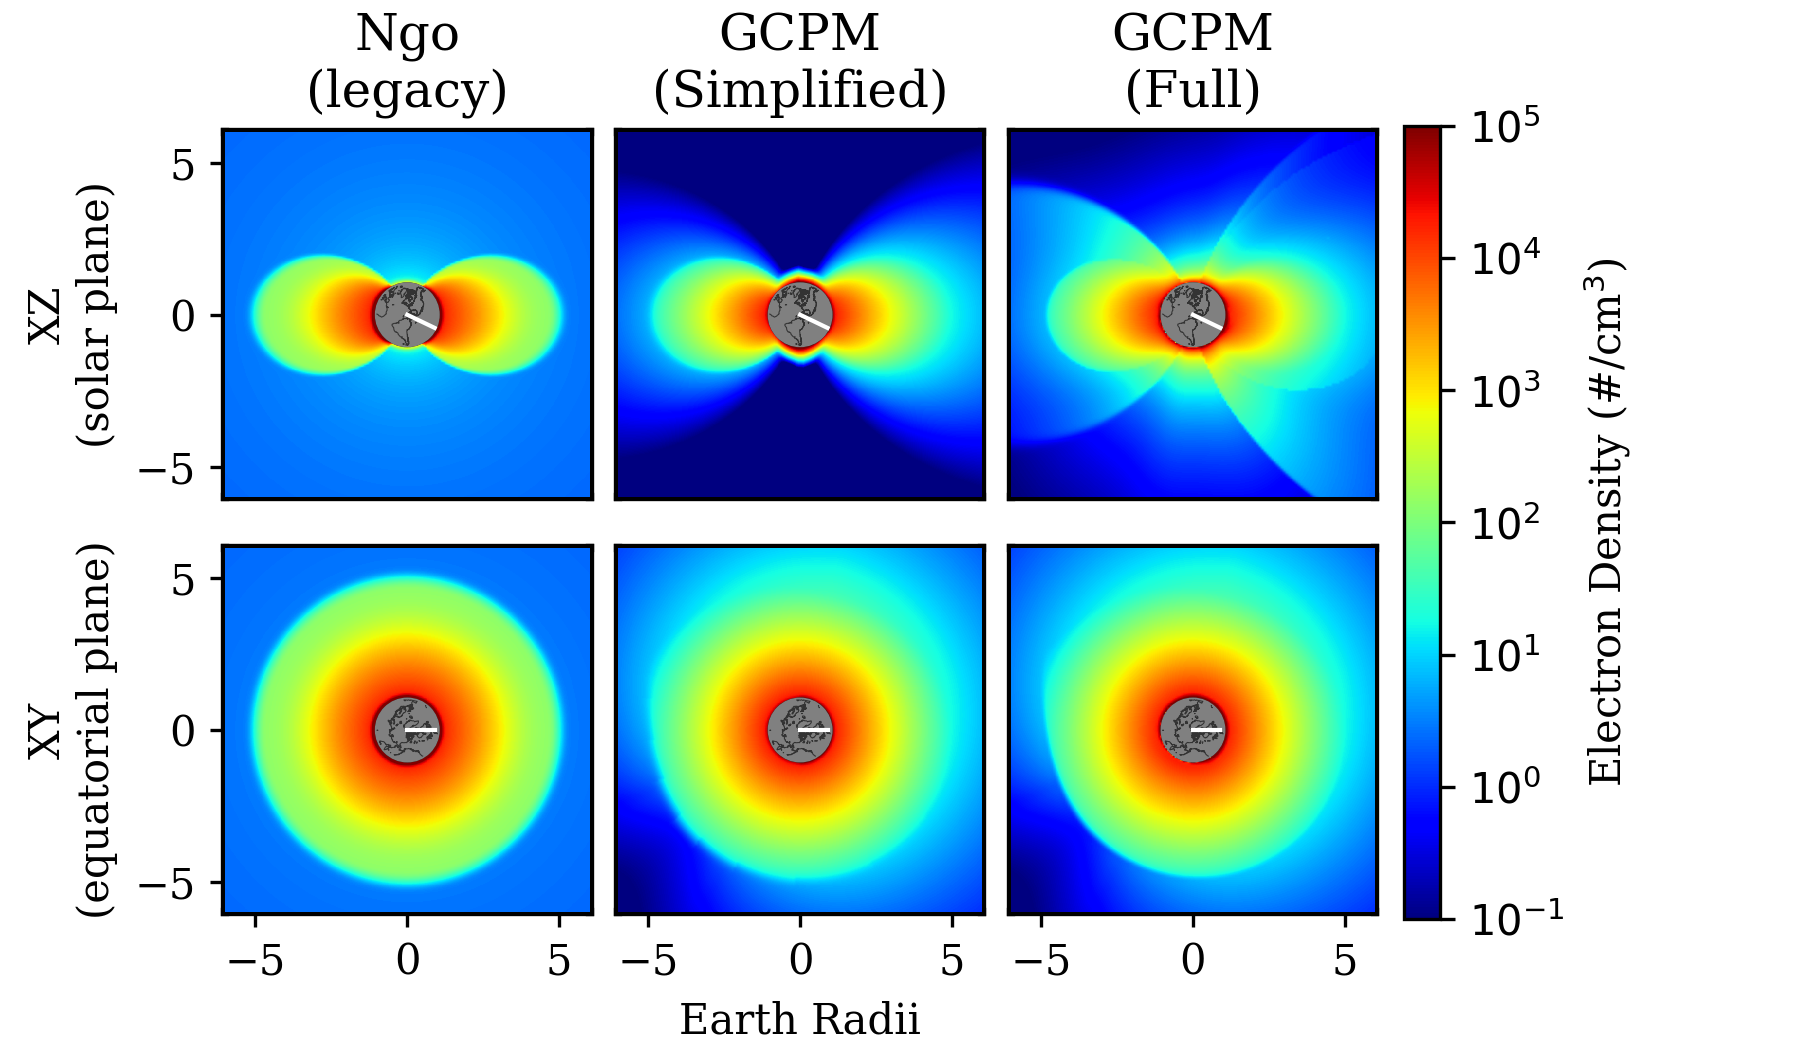
\includegraphics{figures/plasma_model_comparison_serif.png}
%\caption[A Comparison of three plasmasphere electron density models]{A comparison of three plasmasphere models: Ngo, simplified GCPM, and full GCPM, for a relatively quiet plasmasphere ($K_p=2$). The top row shows electron density in-plane with the direction of solar influx; the bottom row shows a top down (equatorial cross-section) view. The white line indicates the solar axis. Only electron density is shown, as additional plasma constituents are derived from electron density.}
%\label{fig:plasma_model_comparison}
%\end{center}
%\end{figure}
%
%\subsection{Ionosphere}
%The ionosphere, extending from $\approx$ 85 km to 1000 km, is the highly-variable transition region between the terrestrial neutral atmosphere and the sparse plasmas of the space environment. In general, our treatment of wave propagation in the ionosphere is abstracted using the method described in section \ref{section:trans_ionosphere_atten}. However, in raytracing through the plasmasphere, we require a smoothly-varying transition between the plasmasphere and ionosphere models.
%
%\paragraph{IRI}
%The International Reference Ionosphere (IRI) is a standard model of several key plasma parameters -- electron density, electron and ion temperatures, ion composition, and so forth. IRI provides detailed outputs as a function of location, altitude, and local time. The GCPM plasma model uses the IRI-2007 implementation \citep{Bilitza2008}; the simplified IRI model is derived from the IRI-2016 model (the most-current available version at time of writing).
%
%\paragraph{Simplified IRI}
%\begin{figure}[h]
%\begin{center}
%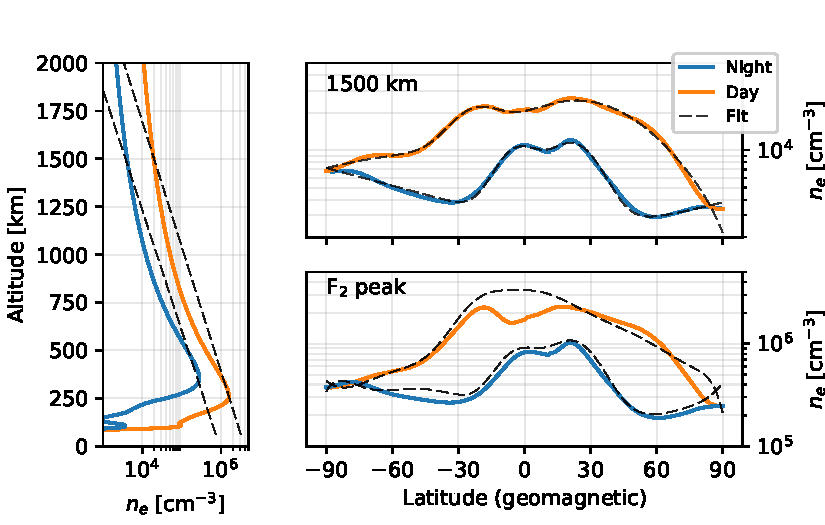
\includegraphics{figures/iono_profile.pdf}
%\caption[Ionosphere density profile]{The IRI electron density model and derived curve fits. The left panel shows electron density variation as a function of altitude, for day and night. The right panels show electron density variation with respect to latitude, for (top) 1500 km and (bottom) the $F_2$ peak (approx. 300 km). Dashed lines indicate the fitted curves used by the simplified IRI model.}
%\label{fig:iono_profile}
%\end{center}
%\end{figure}
%
%In order to both reduce our model parameter space, and to greatly decrease computation time, we pair a simplified version of IRI with a simplified version of GCPM. The IRI-2016 model was run for dayside and nightside ionospheres (12 and 0 MLT), using all default settings, for January 1st, 2000. We then fit a multiple-Gaussian function to the electron density vs latitude, at an altitude of 1500 km, and at the $F_2$ peak. Electron density variation with respect to altitude is approximated by a log-linear fit between 1500 km and the $F_2$ peak. Finally, longitudinal variation is smoothed with a sigmoid function with a width of $\sim$ 1 hr. Figure \ref{fig:iono_profile} shows both the IRI electron density and the derived curve fits.
%

\section{The Radiation Belts}
The term ``Radiation Belts'' or ``Van Allen belts'' refer to the trapped distributions of sparse, very-high-energy electrons, which exhibit two shell-like enhancements which comprise the inner and outer radiation belts. First measured in 1958 by Geiger counters aboard satellites 1958$\alpha$ and 1958$\gamma$ of the Explorer program, the radiation belts were one of the earliest discoveries of the American space program \citep{VanAllen1958}. The vast majority of plasmapshere electrons are ``cold'', and have kinetic energies well under $\sim$ 1 eV. However, radiation belt electrons, while sparse in density, can be highly relativistic, with energies approaching 10 MeV.

Section \ref{section:plasmasphere_density_models} describes the density of electrons and ions in the near-Earth environment. Absent from these models, however, is a discussion of electron and ion energies. The model in section \ref{section:thermal_electron_distributions} assigns an energy distribution to electrons in the $\sim$ 1 eV range to model a warm plasma; the higher energies of radiation belt electrons, however, necessitate a different model.

We model the trapped electron population using the AE8 density model \citep{Vette1991}. AE8 provides omnidirectional, integral fluxes of high-energy electrons as a function of L-shell energy. AE8 is the culmination of several decades of radiation belt studies by the National Space Science Data Center (NSSDC), with the first efforts originating with \cite{Vette1966}. AE8 combines measurements from $\sim$ 94 different instruments across $\sim$ 24 satellite missions from the 1960s and 1970s, which spanned a wide range of orbits, from LEO out to geostationary \citep{Cayton2005}.

Figure \ref{fig:AE8_model} shows the AE8 model output for minimally-populated and maximally-populated conditions. 

\begin{figure}
\begin{center}
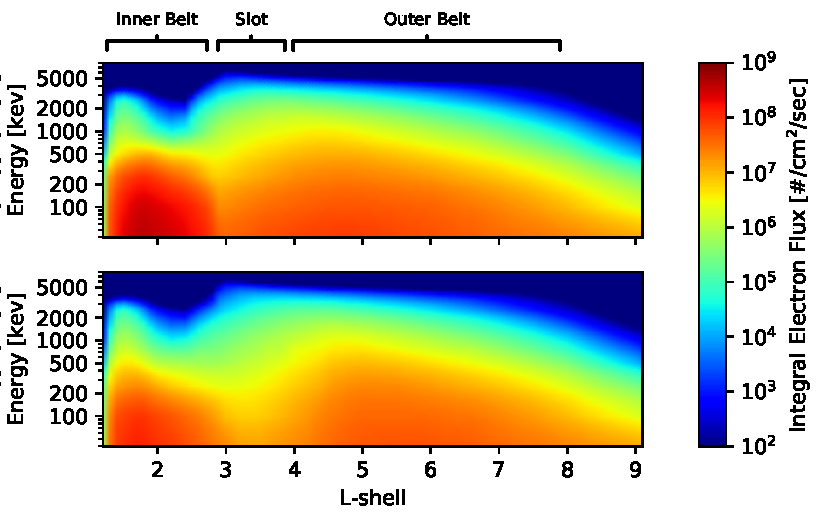
\includegraphics{figures/AE8_fluxes.pdf}
\caption[AE8 integral flux model]{Integral flux for energetic electrons in the radiation belts, as reported by the AE8 model \citep{Vette1991}. The top frame shows the model of maximum conditions, and the bottom frame minimum conditions. The two radiation belts are visible as enhancements within L$\approx$ 2 -- 3 for the inner belt, and L$\approx$ 4 -- 7 for the outer belt. The belts are separated by a depletion known as the ``slot'' region.}
\label{fig:AE8_model}
\end{center}
\end{figure}

The AE8 model reports omnidirectional, integral fluxes -- that is, the total electron flux integrated over a spherical surface -- at the geomagnetic equator. However we require finer detail in directional flux of electrons, which we model via a distribution of pitch angles. \cite{Lauben1998} assumed the simplest distribution, with electrons uniformly-distributed in pitch angle up to the loss cone. \cite{Bortnik2005} compared the square distribution to a more-realistic, sinusoidal distribution. Here we assume a sinusoidal pitch-angle distribution along with the AE8 flux density model. Figure \ref{fig:pitchangledistributions} contrasts the square and sinusoidal distribution functions.


\begin{figure}
\begin{center}
\includegraphics{figures/pitch-angle_distributions.pdf}
\caption[Pitch-angle distribution functions]{Two models of the distribution in pitch angle of radiation belt electrons. The simplest model is a square-shaped distribution, wherein pitch-angles are equally represented within the trapped population. A more realistic model is a sinusoidal distribution. Densities within the loss cone ($\alpha < \alpha_{lc}$) are assumed to be zero.}
\label{fig:pitchangledistributions}
\end{center}
\end{figure}


% RADIATION BELTS



    \chapter{VLF energy in the Near-Earth Environment}
        \label{chapter:power}
    	The purpose of this chapter is to provide a quantifiable assessment of the persistent radio wave energy in the near-Earth space environment due to lightning-generated Whistlers. The morphology of LEP (time evolution, spatial extent at the Earth's surface, and so forth) are primarily determined by the location of wave-particle interactions; additionally, wave-particle interactions with Whistlers are hypothesized to be the primary cause of slot-region electron depletions, and the ``impenetrable barrier'' below L $\sim$ 2.

Lightning-generated Whistlers are sporadic, and exist alongside a multitude of radio wave activity, such as VLF chorus and plasmaspheric hiss, making a correlated \emph{in-situ} measurement challenging. Within this chapter we simulate the relative VLF energy (L-shell, latitude, longitude) in the near-Earth space environment, in volumetric units [J/$m^3$], as a means of assessing their relative contribution to the persistent radio spectrum.

%\section{Overview of Previous Work}

\section{Methodology}
Our simulation is divided into two portions: First, a simulation of persistent VLF energy due to a single flash originating at a fixed latitude, and second, an integration over a measured lightning dataset, using scaled and shifted ``stencils'' for each flash.

Figure \ref{fig:power_blockdiagram} shows the steps required to compute a single stencil. 
\begin{enumerate}
\item{First we model the sub-ionosphere power spectrum generated from a flash with a known peak current, using the methodology of section \ref{section:input_power}.}
\item{We then propagate the energies through the ionosphere, using the attenuating slab approximation method of section \ref{section:trans_ionosphere_atten}.}
\item{We map the effective power above the ionosphere (J/$m^2$ at 1000 km altitude) to an energy density along a fixed grid using a set of pre-computed ``guide rays" using the methodology in section \ref{section:raytracing}, the Landau damping from section \ref{section:damping}, and the novel interpolation scheme described below.}
\item{In order to account for multiple crossings at each grid point, and to reduce our output space across different latitudes, we store the time-averaged energy density along each field line.}
 \end{enumerate}
\begin{figure}
\begin{center}
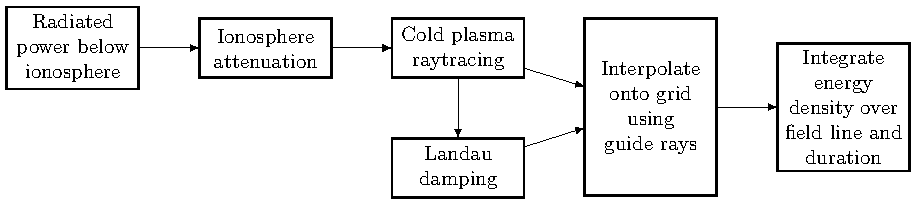
\includegraphics[width=\textwidth]{figures/lightning_power_block_diagram.pdf}
\caption[Energy density calculation block diagram]{Block diagram of the average energy density calculation for a single flash.}
\label{fig:power_blockdiagram}
\end{center}
\end{figure}

\section{Persistent Energy from a Single Flash}

\begin{table}
\caption{Simulation Parameters}
\begin{center}
\begin{tabular}{c|c}
Latitude spacing & 1$^\circ$ \\
Longitude spacing & 1$^\circ$ \\
Frequency range & 200 Hz - 30 kHz \\
Coarse Frequencies & 33 (log-spaced) \\
Fine Frequencies & 20 \\
\end{tabular}
\end{center}
\label{default}
\end{table}%

\subsection{Radiated power above the ionosphere}

% Illumination pattern
\begin{figure}
\begin{center}
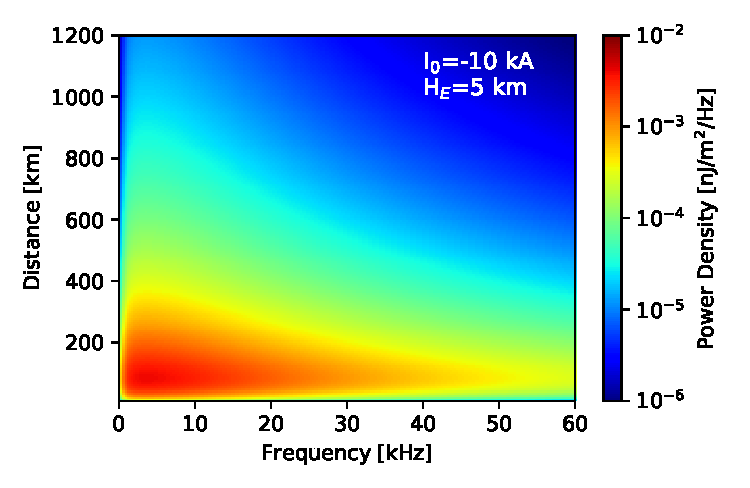
\includegraphics{figures/power_scaling_below_ionosphere.pdf}
\caption[Illumination pattern below the ionosphere]{Vertically-propagating power density from a single discharge, as a function of frequency and radial distance. Adapted from \cite{Marshall2011}.}
\label{fig:illumination}
\end{center}
\end{figure}


% Illumination pattern
\begin{figure}
\begin{center}
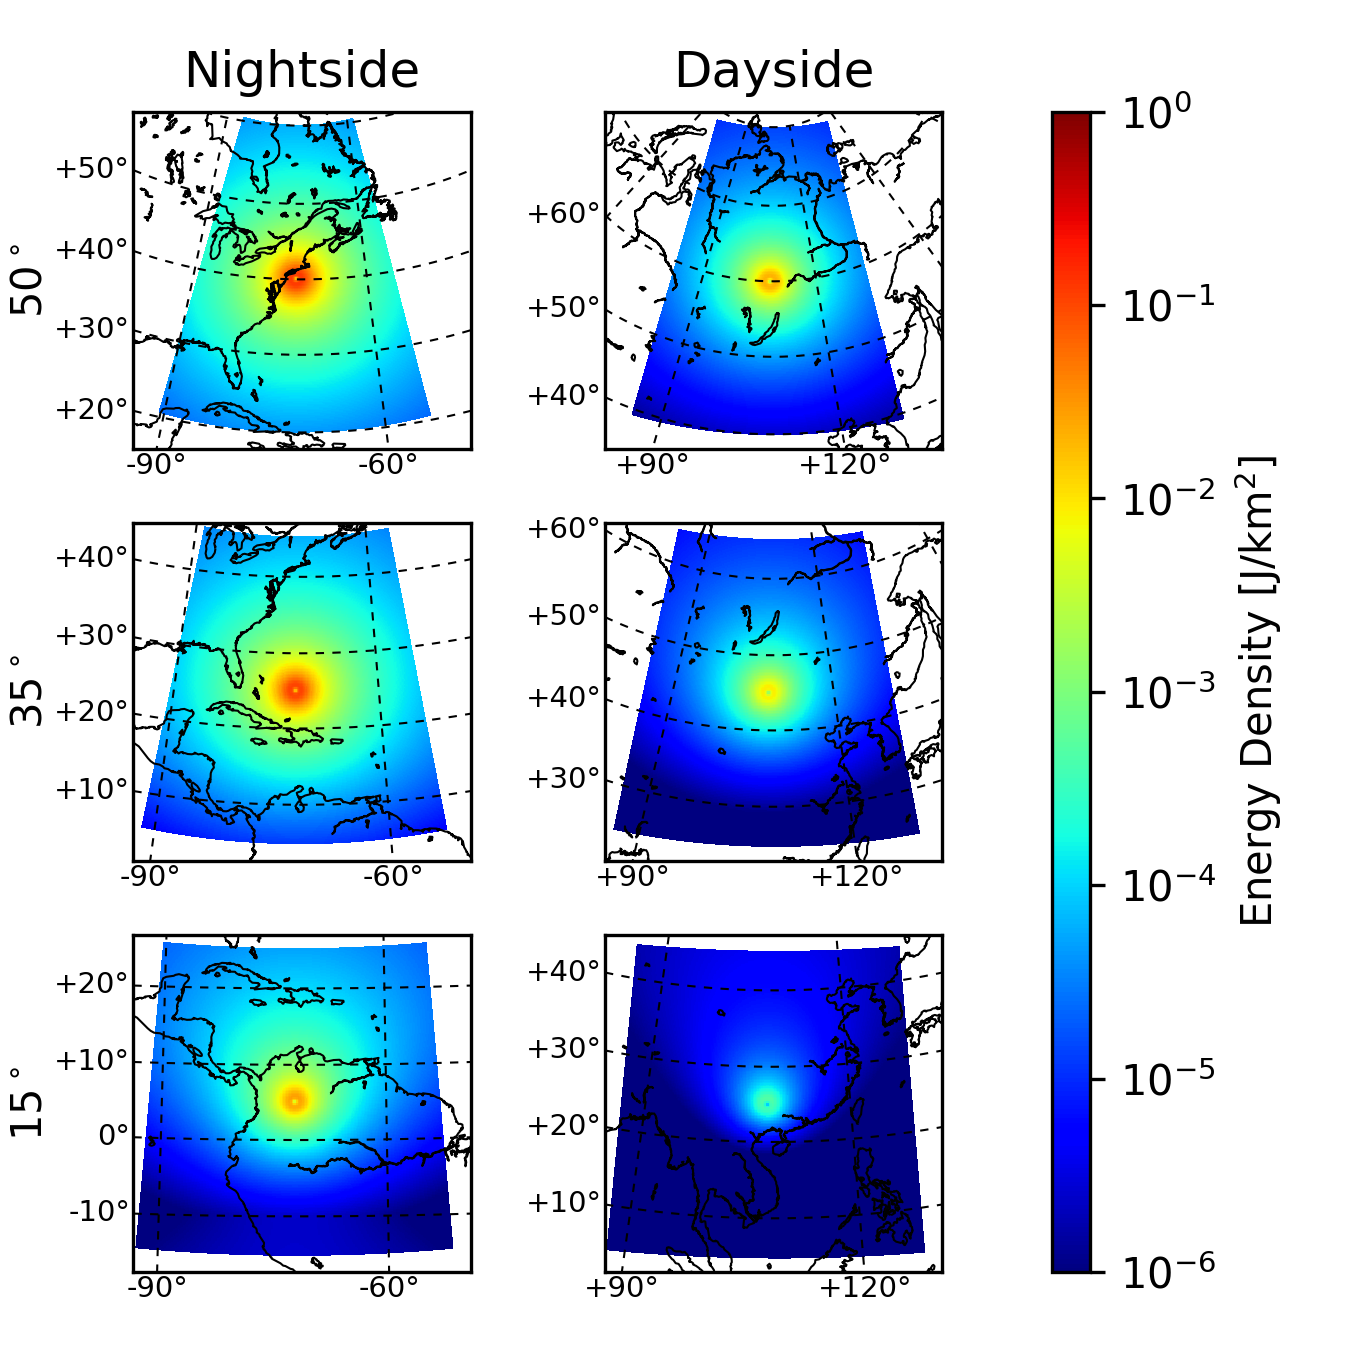
\includegraphics{figures/illumination_basemap.png}
\caption[Illumination pattern above the ionosphere]{Illumination pattern, integrated over frequency, after ionospheric attenuation (altitude = 1000 km).}
\label{fig:illumination}
\end{center}
\end{figure}

% Total energy above ionosphere
\begin{figure}
\begin{center}
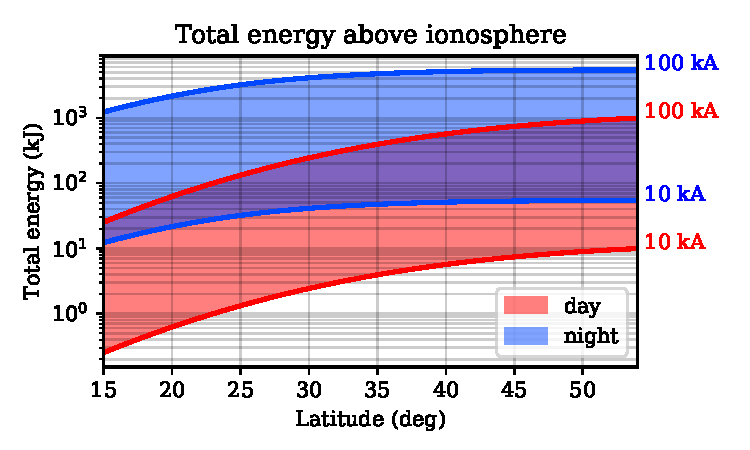
\includegraphics{figures/total_energy.pdf}
\caption[Energy above the ionosphere due to a single flash]{Integrated energy above the ionosphere from a single discharge, as a function of geomagnetic latitude. Energy scales quadratically with peak current; totals for 10 kA (an average flash), and 100 kA (a strong, but not unreasonable flash) are overlaid. }
\label{fig:illumination}
\end{center}
\end{figure}


\subsection{Gridding and Interpolation}

    \begin{figure}
    \centering
    \begin{subfigure}[t]{0.45\textwidth}
    \centering
        	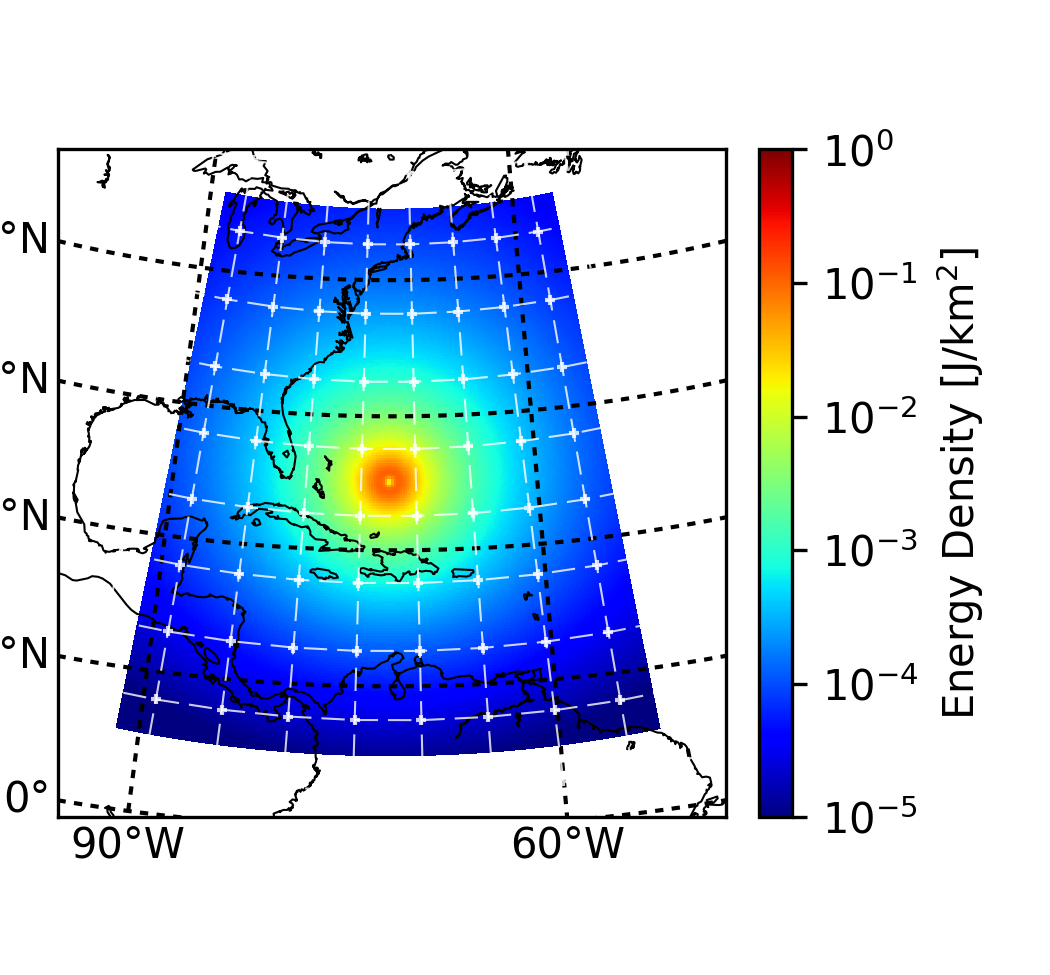
\includegraphics{figures/input_energy_with_grid.png}
	\caption{Input energy gridding}
        \label{fig:input_energy_grid}
    \end{subfigure}\hfill
    \begin{subfigure}[t]{0.45\textwidth}
    \centering
        	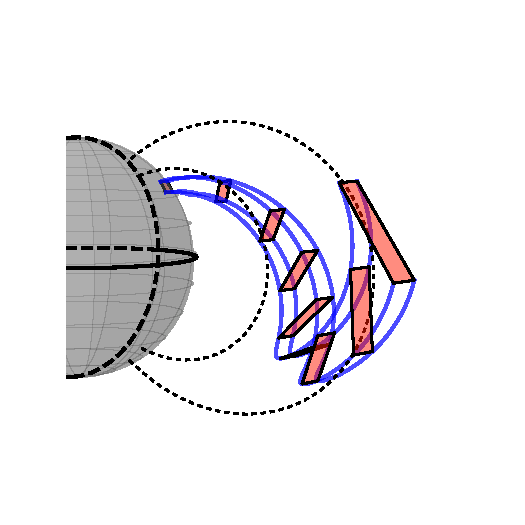
\includegraphics[trim={1cm 0.25cm 1cm 1cm},clip]{figures/interpolation_globe1.pdf}
	\caption{``guide ray'' construction}
        \label{fig:guide_rays}
    \end{subfigure}
    \caption{An illustration of the interpolation scheme. (a) Energy at the top of the ionosphere is divided into cells, in latitude, longitude, and frequency. Shown here with 5$^\circ$ cells (much larger than used in simulation). The plotted energy is integrated over frequency. (b) Illustration of the guide ray method. Input energy is integrated between a set of guide rays, spaced in latitude, longitude, and frequency. This energy is then averaged over a 4-dimensional volume, bounded by two adjacent timesteps $t-1$, $t$ of the guide rays.}
    \label{fig:interpolation_scheme}
\end{figure}


% Delaunay figure
\begin{figure}
\begin{center}
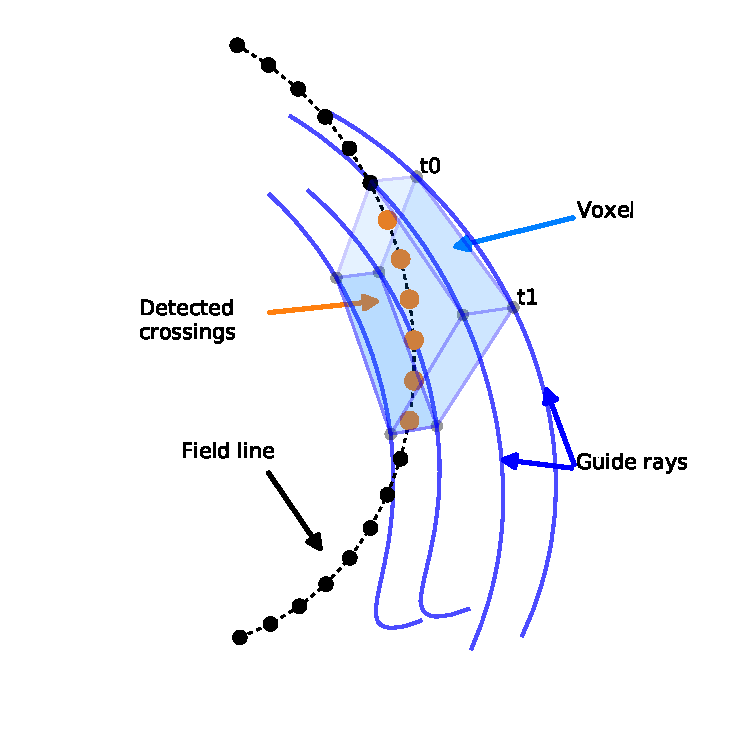
\includegraphics{figures/delaunay_1.pdf}
\caption{Illustration of the Delaunay interpolation method, shown here in three dimensions (e.g., for a single frequency).}
\label{fig:delaunay_1}
\end{center}
\end{figure}

% Fine-scale frequency interpolation
\begin{figure}
\begin{center}
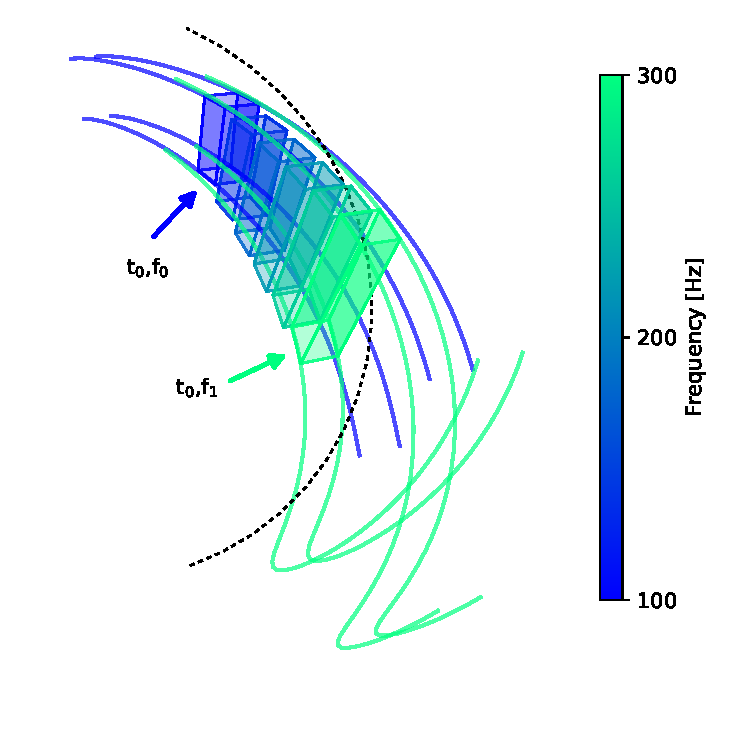
\includegraphics{figures/delaunay_2.pdf}
\caption{Fine-scale frequency interpolation.}
\label{fig:delaunay_2}
\end{center}
\end{figure}

% CONVEX HULL FIGURE
\begin{figure}
\begin{center}
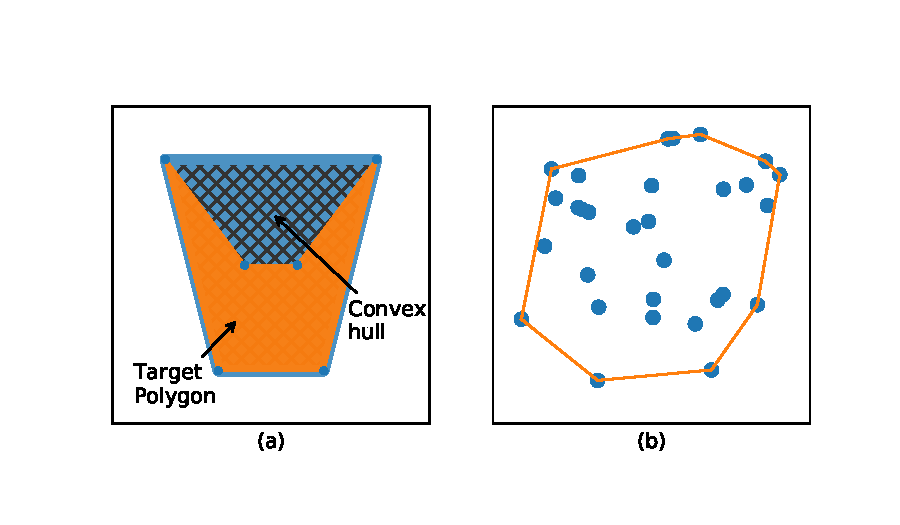
\includegraphics{figures/convex_hulls.pdf}
\caption{Illustration of a convex hull in two dimensions.}
\label{fig:convex_hulls}
\end{center}
\end{figure}



\begin{figure}
\begin{center}
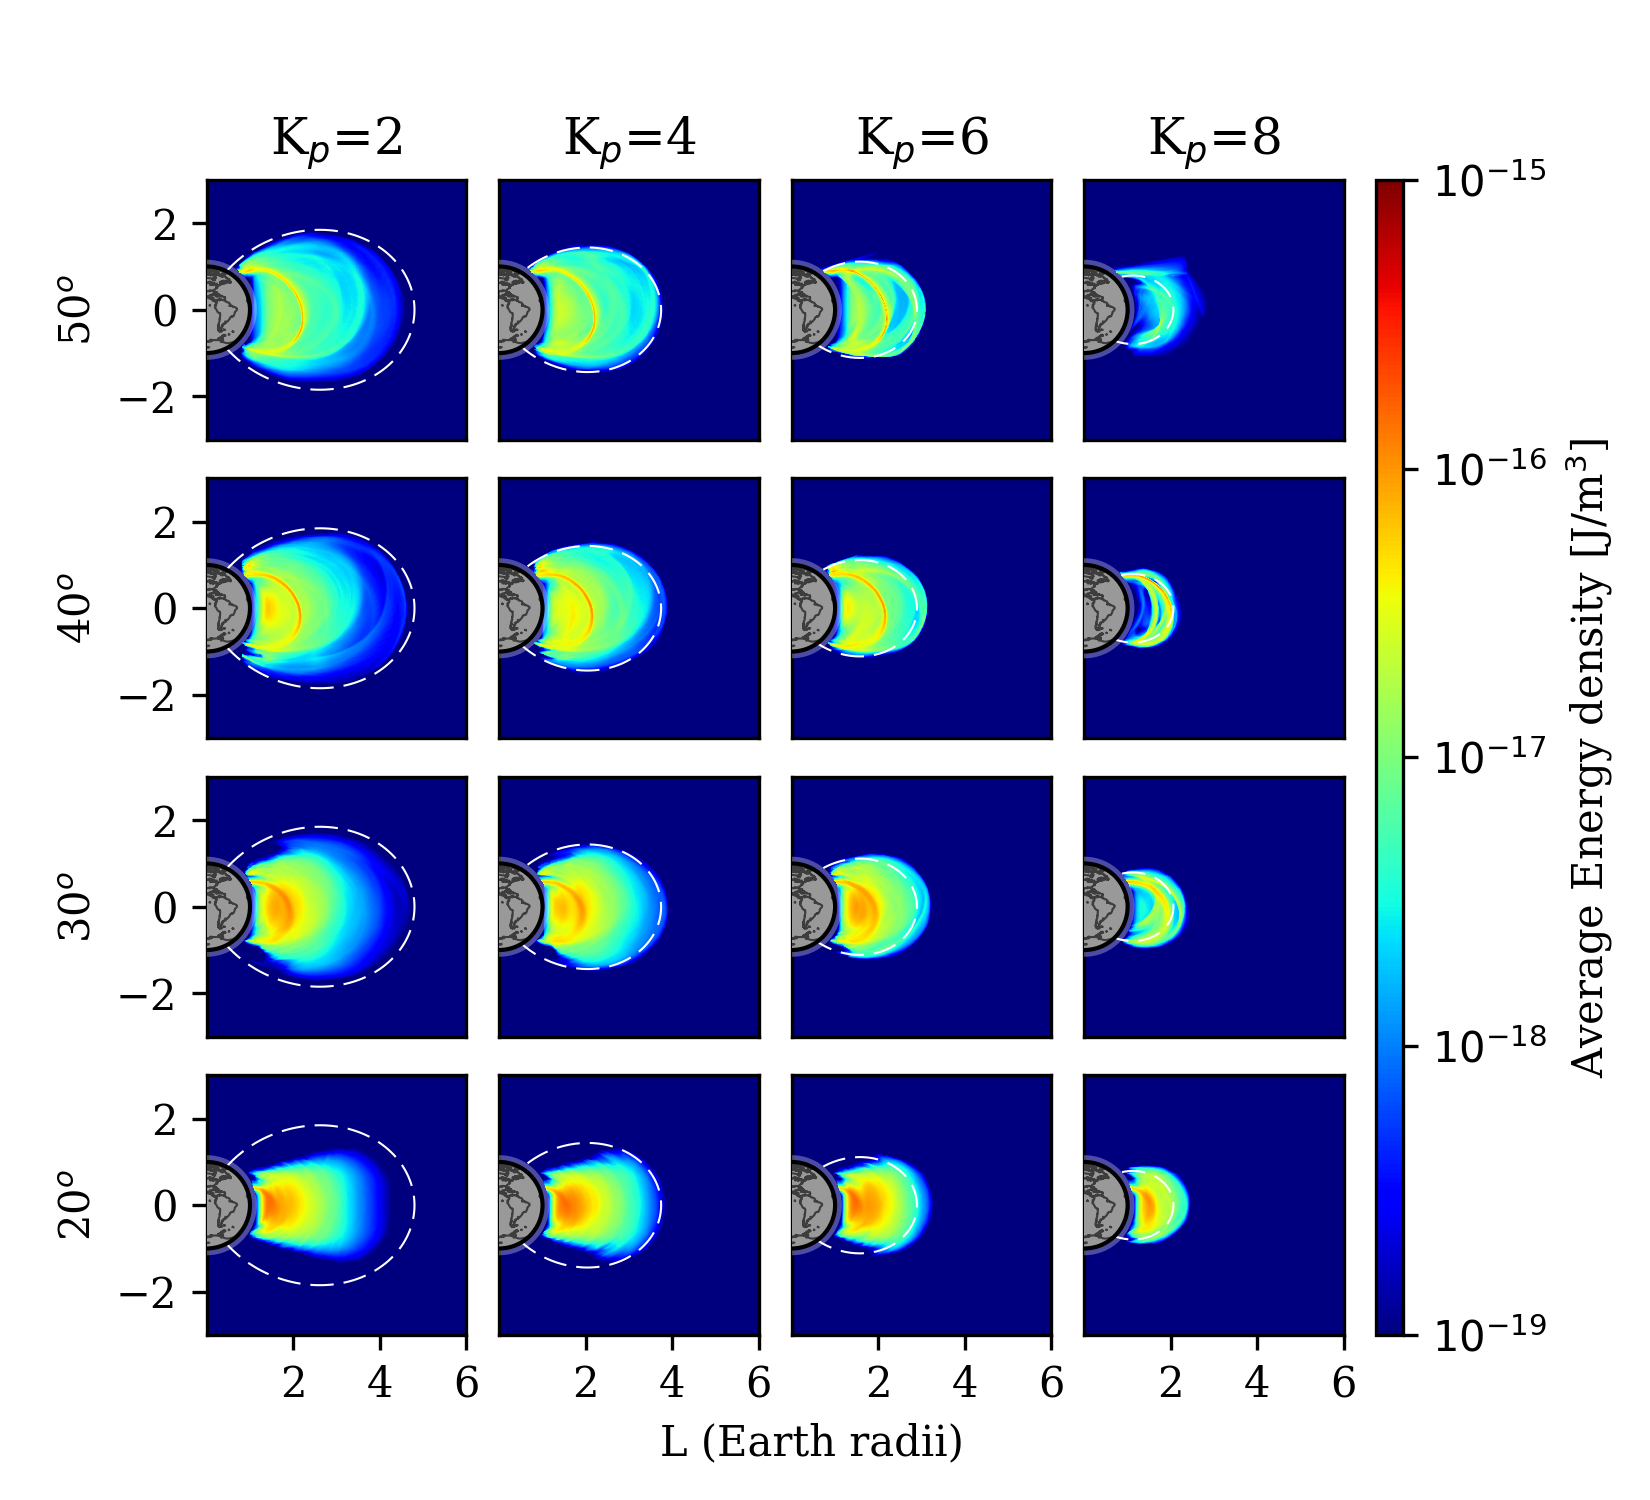
\includegraphics[draft]{figures/energy_from_single_flash_meridonal_plane.pdf}
\caption{Block diagram}
\label{fig:energy_from_single_flash}
\end{center}
\end{figure}

% you'll want to put a figure showing the volume averaging too...

\begin{figure}
\begin{center}
\includegraphics[draft]{figures/energy_in_meridional_plane_movieframes.pdf}
\caption{Block diagram}
\label{fig:energy_from_single_flash}
\end{center}
\end{figure}


\begin{figure}[ht]
\begin{center}
\includegraphics[draft]{figures/energy_stencils.pdf}
\caption{Block diagram}
\label{fig:energy_stencils}
\end{center}
\end{figure}

\section{Global Energy Density}

\begin{figure}
\begin{center}
\includegraphics[draft]{figures/energy_density_vs_L_vs_freq.pdf}
\caption[Average energy density vs L and frequency]{Average energy density as a function of L-shell and wave frequency}
\label{fig:energy_density_vs_L_vs_freq}
\end{center}
\end{figure}


    \chapter{3D Modeling of LEP}
        \label{chapter:3dWIPP}
  	\section{Overview of Previous Work}

    \chapter{Global and Seasonal Estimates of LEP}
        \label{chapter:global_estimates}
    	The purpose of this chapter is to provide quantitative upper and lower-bound estimates on the expected electron flux due to LEP, as a function of location and time of year. We expand on the raytracing and interpolation method described in chapter \ref{chapter:power}, by incorporating a resonant-particle scattering code. We compute global electron fluxes in a similar manner as in Chapter \ref{chapter:power}, using an array of precomputed stencils, which we scale and shift according to GLD360 data. Finally, we can examine the relative timescales on which LEP could deplete a populated magnetic field line, in the absence of any other loss processes.

\section{Resonant Interactions}
As discussed in section \ref{section:wpi}, the interaction between waves and trapped particles has a cumulative effect only when certain resonant conditions are met. The condition for resonance is given by:
\begin{equation}
\frac{d\eta}{dt} = m \omega_c/\gamma - \omega - k_z v_z = 0
\label{eqn:resonance_cond}
\end{equation} 
where m is the resonance order number, $\gamma = (1 - v^2/c^2)^{-1/2}$ is the Lorentz relativistic correction factor, $\omega_c$ is the local cyclotron frequency, and $k_z$ and $v_z$ are the parallel components of the wavenormal vector and particle velocity with respect to the background magnetic field. The angle between the wave magnetic field vector and $v_\perp$ is given by $\eta$.

We assume any perturbation in pitch angle is small, and can therefore only concern ourselves with particles very near the edge of the loss cone. We can therefore relate the total velocity $v$ and the parallel velocity $v_z$ via $v^2 = v_z^2/\cos^2\alpha_{lc}$ \citep{Lauben2001, Bortnik2006}.

Plugging in the above terms for $\gamma$ and $v_z$ gives us the following closed-form expression for the resonant particle velocity for an incident wave:
\begin{eqnarray}
v_z^{res} & = & \bigfrac{\pm \sqrt{\omega^2 k_z^2 + \left[ (m \omega_c)^2 - \omega^2 \right] \left[k_z^2 + (\frac{m \omega_c}{c \cos \alpha_{lc}})^2\right]} - \omega k_z}{k_z^2 + (\frac{m \omega_c}{c \cos \alpha_{lc}})^2} \unit{m/sec}
\label{eqn:vzres}
\end{eqnarray}

The resonant kinetic energy can then be related by:
\begin{eqnarray}
v_z^{res} = \|v_{res}\|\cos\alpha_{lc}  \unit{m/sec}\\ 
E_{res} = \frac{E_{0}}{\sqrt{1 - v_{res}^2/c^2}} - 1 \unit{J}
\end{eqnarray}

\noindent where $E_{0}$ is the particle rest energy ($\approx$ 511 keV for an electron).

Equation \eqref{eqn:vzres} is a function of the incident wave, which is dependent on the wavenormal angle and the background plasma through $k_z$. We can illustrate broad trends by plotting resonant frequency vs kinetic energy along the geomagnetic equator, for normal incidence ($k = k_z$). Figure \ref{fig:vzres_vs_modes} shows the resonant frequency for a range of L-shells, for m = $\{0,1,2\}$. Somewhat counterintuitively, lower-energy particles resonate with higher-frequency waves.

L-shell dependence is due both to the background electron density through $k_z$, and the background magnetic field through $\omega_c$. Particles at higher L-shells resonate with lower-frequency waves.

\begin{figure}[h]
\begin{center}
%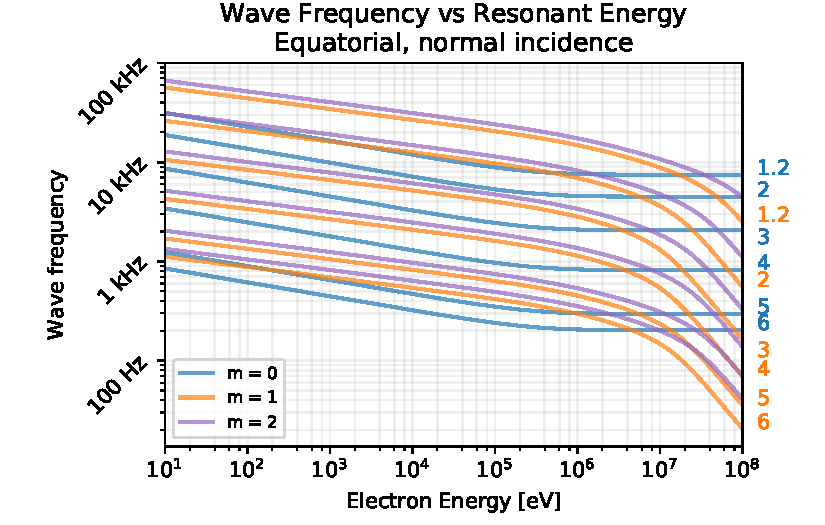
\includegraphics{figures/wave_frequency_vs_energy_vs_mode.pdf}
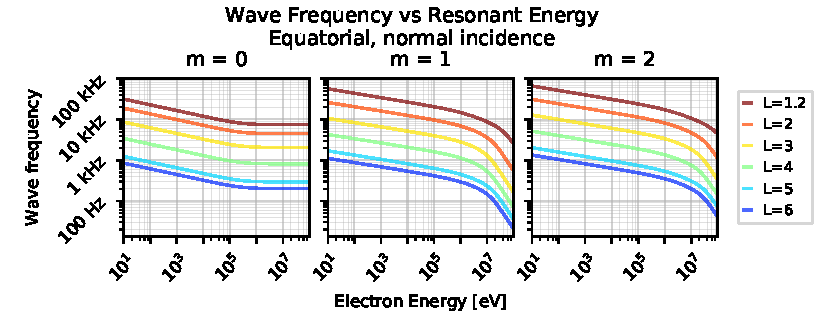
\includegraphics{figures/wave_frequency_vs_energy_vs_mode_3up.pdf}

\caption[Resonant frequency vs particle energy for resonant modes 0, 1, and 2]{Resonant wave frequency vs trapped electron kinetic energy, for resonant modes m = 0, 1, and 2. Shown here for resonances along the geomagnetic equator, with normal incidence. The background plasma is modeled for \kp{}=0 using the Simplified GCPM model in section \ref{section:plasmasphere_models}.}
\label{fig:vzres_vs_modes}
\end{center}
\end{figure}

At lower energies, the resonant modes are integer multiples of each other; however as the particles become increasingly relativistic, the modes deviate substantially. Most significantly, when setting $m=0$, the relativistic term vanishes completely, and the resonant frequency asymptotes.

\subsection{Calculating pitch-angle scattering vs time}

Calculating pitch-angle perturbations incurs additional complexity as compared to the energy density estimate in Section \ref{chapter:power}. Pitch-angle scattering is dependent on wave amplitude and frequency, as well as incident wavenormal angle $\theta$ and gyrophase $\eta$. Additionally, the formulation for pitch-angle scattering requires wave amplitudes with units of (Poynting) energy flux, $\mathrm{1/m^2/s}$, rather than volumetric densities, $\mathrm{1/m^3}$.

The fundamental pitch-angle scattering equation is given in equation \eqref{eqn:bell_dadt}, and reproduced below:
\begin{equation}
\frac{d\alpha}{dt} = \underbrace{\frac{m_e \omega_{\tau m}^2}{k_z p_\perp} \bigg( 1 + \frac{\cos^2\alpha}{m\,\omega_c / \omega - 1}\bigg)}_{T_1}\underbrace{\sin \eta}_{T_2} + \underbrace{\frac{1}{m_e \gamma}\frac{p_\perp}{2 \omega_c}\frac{\partial \omega_c}{\partial z}}_{T_3} \unit{rad/sec}
\label{eqn:bell_dadt_with_labels}
\end{equation}

Terms $T_1$ and $T_3$ are slowly-varying, and can be treated as pseudo-constant at a fixed position in space. Term $T_2$ in \eqref{eqn:bell_dadt_with_labels} is the resonant component. Outside of resonance this term oscillates between $\pm 1$. At resonance, however, this term remains constant, allowing coherent changes to accumulate over the interaction period. Resonance implies only that $d\eta/dt = 0$, and provides no information on the value of $\eta$. We assume $\eta$ is uniformly distributed, in which case the perturbation in pitch angle $d\alpha/dt$ will be sinusoidally distributed, symmetrically about zero \citep{Inan1977}. Since we are concerned only with the distribution of particles which are perturbed into the loss cone ($d\alpha/dt < 0$), we can then track the RMS-average pitch angle change $\Delta \alpha_{RMS}$, and calculate the precipitated fraction using the uniform distribution (see section \ref{section:flux_from_pitch_angle}).
Figure \ref{fig:test_particle_sims} shows an example of a test-particle simulation, in which a set of particles with different initial $\eta$ values are subjected to the same perturbing wave.

\begin{figure}[t]
\begin{center}
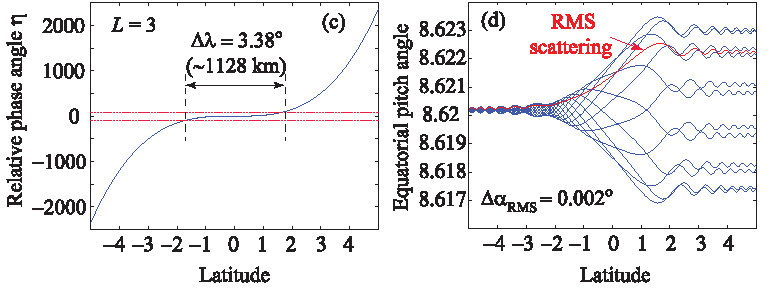
\includegraphics{figures/Bortnik_RMS_scattering.pdf}
\caption[RMS pitch angle scattering from a test particle simulation]{Comparison of RMS and peak deflection in pitch angle from a test particle simulation. On the left is shown the relative gyrophase angle, which must be constant in order for changes to accumulate. On the right is the pitch angle of an array of particles, each with a different initial gyrophase. After the interaction has occurred, the perturbed pitch angles are symmetric about the initial pitch angle. The red curve shows the RMS change. Figure taken from \cite{Bortnik2006}, Figure 7.}
\label{fig:test_particle_sims}
\end{center}
\end{figure}

From here, we follow the numerical solution method from \cite{Bortnik2005, Bortnik2006}. 

A key assumption in our scattering calculation is that the interactions on a single particle from each discrete frequency are independent from one another. Furthermore, we discretize each fieldline into 1$^\circ$ segments, and assume the scattering within each segment is independent from each other. While neither of these assumptions are exactly true, together they provide a critical and substantial reduction in complexity: we no longer have to track the action of the entire set of waves on a discrete set of particles (as in a test particle simulation such as \cite{Chang1985}), but rather can track the stochastic pitch-angle change on a distribution of particles. Additionally, by assuming incoherent scattering across frequencies, the problem becomes much more well-suited to a parallel processing solution, as we can spread computation for each frequency across an array of nodes.\footnote{The coherent-incoherent assumption is based on test particle simulations such as \cite{Chang1985} and \cite{Ristic1993}; however a modernized test-particle (time domain) validation of the approach would be an excellent opportunity for future work!}

Thus, for each set of guide rays $F$, using the interpolation scheme from section \ref{chapter:power}, we can calculate $\Delta \alpha_{RMS}$ as a function of magnetic fieldline, particle energy, and time; the effective change in pitch angle is then determined by summing over the set in quadrature: 
\begin{equation}
\Delta \alpha(E, \vec{x}, t) = \frac{1}{2}\sqrt{\sum_{F} \Delta \alpha_{RMS}^2(E, \vec{x},t, F)}.
\end{equation}

The decision to calculate RMS pitch-angle scattering versus a full test-particle approach is the fundamental difference between \cite{Lauben1998} and \cite{Bortnik2005}, the two most-closely related works to ours. \citeauthor{Bortnik2005} uses the above method, while \citeauthor{Lauben1998} infers expected distributions from a set of test particles. 

As noted by \cite{Lauben1998, Lauben2001}, a subset of particles, when subjected to ideal conditions, can ``ride'' a perturbing wavefront across several degrees in latitude, and experience sustained, coherent perturbation. These particles would then precipitate very deeply into the ionosphere, which may account for the lowest-altitude ionization as measured using VLF sub-ionosphere sensing. However these particles represent only a small fraction of the precipitating electrons, the bulk of which experience a random walk through the set of perturbing waves, and are well-modeled by the stochastic RMS formulation of \citeauthor{Bortnik2005}.

\citeauthor{Bortnik2005} makes several approximations which allow for quick numerical integration of \eqref{eqn:bell_dadt_with_labels}, the details of which are beyond the scope of this dissertation. For a concise description of the methodology, see \cite{Bortnik2006}. Table \ref{alg:RMS_change} shows the algorithm in pseudocode. Using the assumptions of incoherence described above, we can independently calculate squared pitch-angle change for every enumerated combination of: a) guide ray sets $F$, b) latitudes along an output fieldline $\lambda$, c) time steps $t$, d) resonant modes $m$, and e) resonant particle energies $E$. 

\begin{algorithm}[t]
\caption{RMS change in pitch angle}\label{alg:RMS_change}
\begin{algorithmic}[1]
\ForAll{output field lines}
	\State{d$\alpha$\_N $\gets$ Zeros(E, t)}\Comment{Pitch angle change at northern hemisphere}
	\State{d$\alpha$\_S $\gets$ Zeros(E, t)}\Comment{Pitch angle change at southern hemisphere}
	\ForAll{sets of guide rays}
		\State{Scale input energy according to input flash location and frequency}
		\ForAll{latitudes along field line $\lambda$}
			\ForAll{time steps $t$}
				\ForAll{resonant modes $m$}
					\State{Calculate $V_{res}$, $E_{res}$}
					\ForAll{grid energies within resonance band $E$}
						\State{$\Delta \alpha_{cur} \gets \int_{t1}^{t2} \frac{d\alpha}{dt}$}
						\State{tN $\gets$ t + $\tau_{f,N}$} \Comment{flight time to northern ionosphere}
						\State{tS $\gets$ t + $\tau_{f,S}$} \Comment{flight time to southern ionosphere}
						\State{d$\alpha$\_N[E, tN] += $(\Delta \alpha_{cur})^2$}
						\State{d$\alpha$\_S[E, tS] += $(\Delta \alpha_{cur})^2$}
					\EndFor
				\EndFor
			\EndFor
		\EndFor
	\EndFor
	\State{d$\alpha$\_N $\gets \sqrt{\mathrm{d}\alpha\_\mathrm{N}}$}
	\State{d$\alpha$\_S $\gets \sqrt{\mathrm{d}\alpha\_\mathrm{S}}$}
\EndFor
\end{algorithmic}
\end{algorithm}


To account for variation in precipitation time, we record the perturbation in pitch angle at the time in which a perturbed particle would precipitate into the atmosphere. This time is dependent on both particle energy and the latitude along the field line where the perturbation occurred, and may be asymmetric between the northern and southern hemispheres.

We compute the time of flight from the interaction latitude $\lambda$ to the ionosphere by assuming a perturbed particle continues along a fixed fieldline, by numerically evaluating the expression from \cite{Walt1994}, equation 4.25:

\begin{equation}
\tau_f =  \frac{1}{v} \int_{s_1}^{s_2} \bigg(1 - \frac{B(s)}{B_{eq}}\sin^2\alpha_{eq}\bigg)^{-1/2} \mathrm{d}s
\label{eqn:bounce_time}
\end{equation}

\subsection{Example energy-time spectra}
Figure \ref{fig:dA_spectra} shows a typical pitch-angle scattering matrix, as a function of electron energy and time delay from a lightning flash at $35^\circ$ latitude, with $I_0=-10$kA. A similar scattering matrix must be computed for every point in the output space (L-shell and longitude offset).

\begin{figure}[h]
\begin{center}
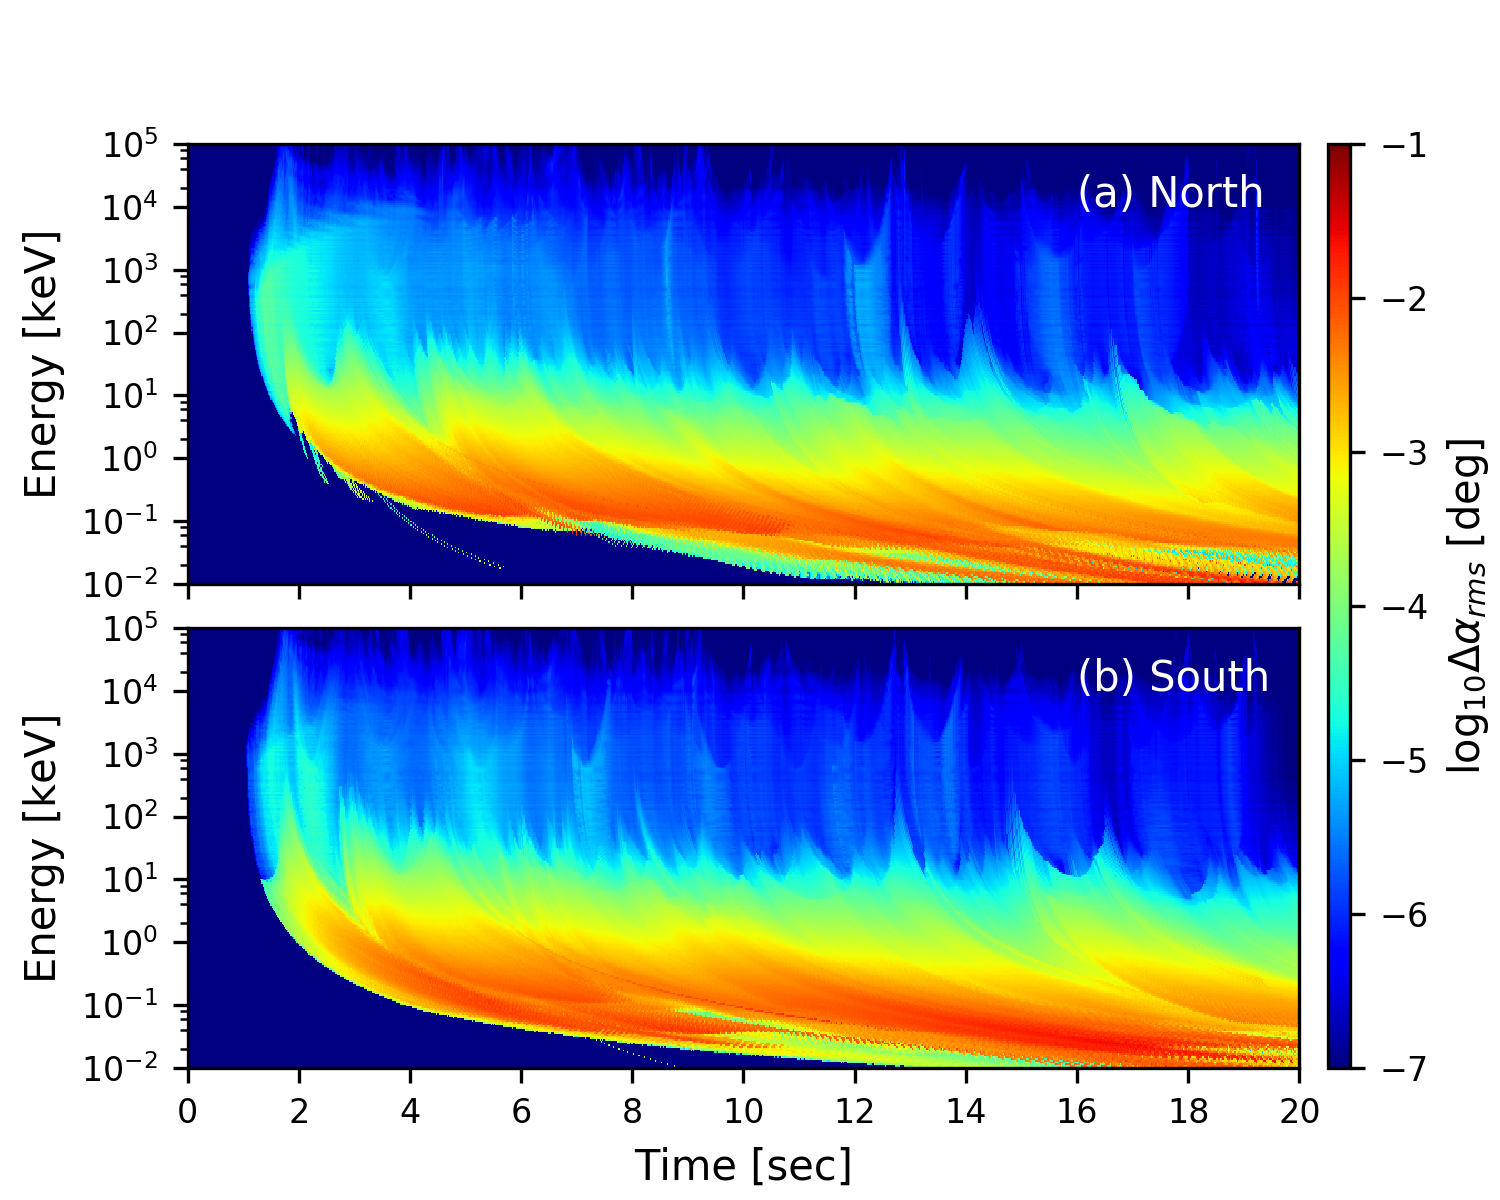
\includegraphics{figures/dA_E-t_spectra.png}
\caption[Pitch angle scattering matrix for a flash at 35$^\circ$ latitude and L=3]{Pitch angle scattering matrix along a fieldine with L=3, for a 10 kA flash at 35$^\circ$ latitude, through a nightside ionosphere at \kp{}=0. Scattering is centered directly over the input flash longitude, within a width of $\pm0.25^\circ.$}
\label{fig:dA_spectra}
\end{center}
\end{figure}

Several key features are apparent: First, the descending curve shape is due to the time delay from the interaction region to the precipitation altitude, with slower moving electrons taking longer to reach the ionosphere. Two banded structures are visible with respect to energy: the dominant band, below $E \sim 10$ keV, is due to the 0-order resonance mode. The upper band with energies above $E  \sim 100$ keV, is due largely to the $\pm$ 1 resonance modes. Scattering efficiency decreases with increasing resonance order, due to the presence of order number $m$ in the denominator of equation \eqref{eqn:bell_dadt_with_labels}, term T1. While some asymmetry exists between the northern and southern hemispheres, the magnitude remains similar due to the numerous bounces of the incident waves, and because the higher-order modes resonate with particles traveling in either direction.

Perturbations in pitch angle due to LEP are generally small; well below $0.1^\circ$. However, due to the exponentially-increasing density of the ionosphere below our threshold height of 100 km, and thus the very small change in reflection altitude required, small changes in pitch angle can greatly increase an electron's likelihood of precipitating. Figure \ref{fig:pitch_angle_vs_altitude}(a) shows the perturbed reflection altitudes versus L-shell, for an array of $\Delta \alpha$ values. Figure \ref{fig:pitch_angle_vs_altitude}(b) shows the minimum perturbation value required in order for a particle to reflect at a given altitude.

\begin{figure}[t]
\begin{center}
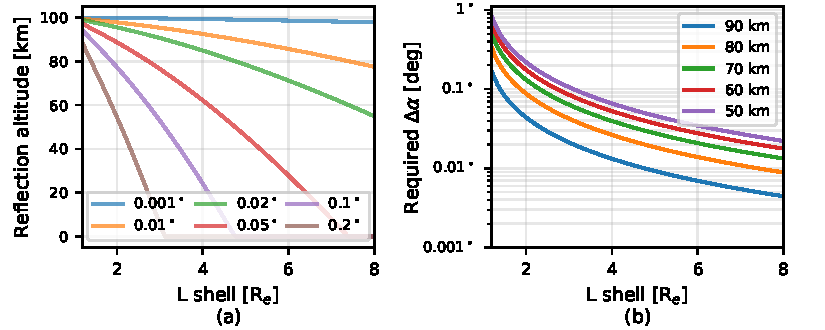
\includegraphics{figures/pitch_angle_vs_depth.pdf}
\caption[Reflection altitudes vs L-shell for a set of pitch angle perturbations]{(a) Reflection altitude vs L-shell for a particle, for an array of equatorial pitch-angle perturbations. (b) The minimum perturbation required to drive a particle with pitch angle $\alpha = \alpha_{lc}$ to a fixed reflection altitude, as a function of L-shell, for an array of target altitudes.}
\label{fig:pitch_angle_vs_altitude}
\end{center}
\end{figure}


\section{Calculating flux from pitch-angle perturbations}
\label{section:flux_from_pitch_angle}
We have now computed the RMS change in pitch angle along a single field line, as a function of electron energy and time, for a single lightning flash. Next we must convert our scattering matrices (Figure \ref{fig:dA_spectra}) into electron fluxes (or energy fluxes). Again, we follow the method used by \cite{Bortnik2005} (section 5.1.3).

Along each target fieldline, we use our calculated pitch angle changes $\Delta \alpha(E,t)$ to perturb a collection of electrons with an assumed distribution in pitch angle. Perturbation is accomplished by convolving an assumed distribution of particles $G(E,t,\alpha)$ with the perturbing function $\Delta \alpha(E,t)$ for each energy and time bin. The resulting particle flux is the number of electrons within the loss cone ($\alpha < \alpha_{lc}$) after perturbation. We assume that scattering is independent with respect to both the time and energy axes, and can thus be evaluated independently for each $E-t$ bin. Solving the convolution analytically greatly improves computational efficiency.

We use the solution from \cite{Bortnik2005} for a ``ramp'' distribution in pitch angle, which can be applied to any general pitch angle distribution by computing a series approximation about $\alpha = \alpha_{lc}$.

\begin{equation}
% Bortnik figure 5.8, equation d.  
% Maybe you should include a figure here too?
\end{equation}


\begin{figure}[t]
\begin{center}
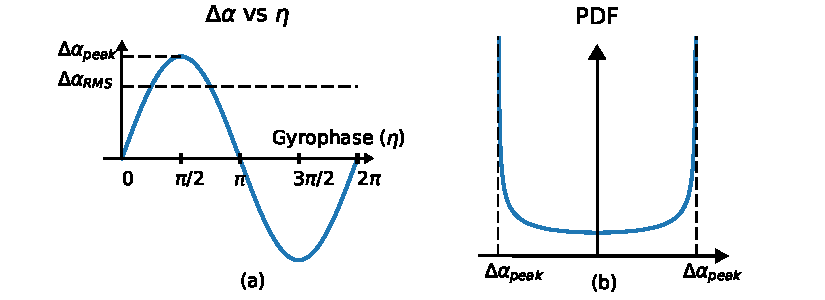
\includegraphics{figures/da_dist_and_pdf.pdf}
\caption[Pitch angle perturbation vs gyrophase, and corresponding PDF]{(a) Pitch angle perturbation vs particle gyrophase, with $\Delta \alpha_{rms}$ marked, and (b) The corresponding probability density function (PDF, equation \eqref{eqn:pdf}). Modified from \cite{Bortnik2005}, Figure 5.8.}
\label{fig:da_vs_eta_and_pdf}
\end{center}
\end{figure}

\begin{figure}[h]
\begin{center}
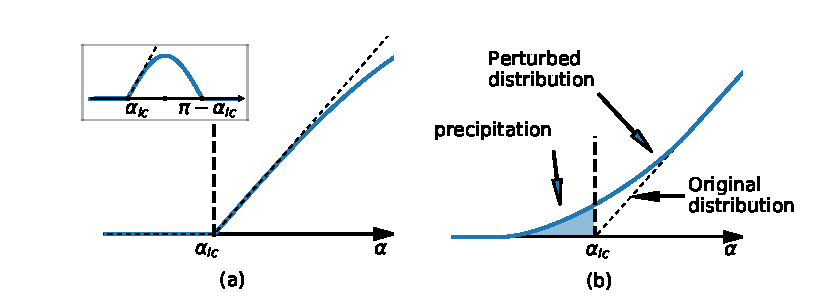
\includegraphics{figures/da_dist_and_perturbation.pdf}
\caption[Perturbed pitch-angle distribution]{(a) The initial pitch-angle distribution function and its linear expansion at $\alpha = \alpha_{lc}$. (b) The perturbed distribution, resulting from the convolution of plot (a) with \ref{fig:da_vs_eta_and_pdf}(b). The shaded region indicates particles which have been pushed into the loss cone ($\alpha < \alpha_{lc}$). Modified from \cite{Bortnik2005}, Figure 5.8.}
\label{fig:da_dist_and_perturbation}
\end{center}
\end{figure}

Implicit in this calculation is the distribution in gyrophase, which is taken to be uniform. This allows us to use our RMS pitch angle perturbations in place of an explicit distribution of perturbations across gyrophase. Figure \ref{fig:da_vs_eta_and_pdf} (a) shows the assumed pitch-angle perturbation as a function of gyrophase, $\eta$, and $\Delta \alpha_{RMS}$. We then convert this distribution to its cumulative distribution function F$(\alpha)$, and its probability density function $f(x)$, shown in Figure \ref{fig:da_vs_eta_and_pdf} (b):

\begin{eqnarray}
F(\alpha) & = & P(X < \alpha) = \int_{-\infty}^\alpha f(x) dx \nonumber \\
& = & P((\Delta \alpha_{peak}\sin Y) < x) \nonumber \\
& = & P(Y < \arcsin(x/(\Delta\alpha_{peak})) \nonumber \\  
& = & \frac{\arcsin(\alpha/(\Delta\alpha_{peak}))}{\pi} + \frac{1}{2}  \\
 f(x) & = & \frac{\mathrm{d}F(\alpha)}{\mathrm{d}x} = \frac{1}{\pi\sqrt{(\Delta \alpha_{peak})^2 - (\alpha)^2}}
 \label{eqn:pdf}
\end{eqnarray}

While $\Delta \alpha(E,t)$ is computed only for particles at the edge of the loss cone, $\alpha = \alpha_{lc}$, we note that the perturbation varies slowly with respect to initial pitch angle, and that only particles within $\sim 0.1^\circ$ of the loss cone will be scattered into the loss cone, and can therefore apply the same perturbation to the distribution of electrons just inside the loss cone.

The unperturbed particle population is modeled by:
\begin{equation}
G(E,t,\alpha) = G_1(E, t_0)G_2(\alpha)
\label{eqn:background_density}
\end{equation}
where $G_2(\alpha)$ is the dependence on pitch angle, and $G_1(E, t_0)$ is the energy-differential electron flux at the equator for a given energy band $E$, and time of day $t_0$, along the target field line.

We model $G(\alpha)$ with a sinusoidal distribution between $\alpha=\alpha_{lc}$ and $\alpha = \pi - \alpha_{lc}$, as in Figure \ref{fig:pitchangledistributions}. The background radiation belt density $G(E,t_0)$ is modeled using the AE8 numerical model for both maximal and minimal filling, as in Figure \ref{fig:AE8_model}.

The perturbed flux density $\Phi(E,t,\alpha)$ is given by convolving equations \eqref{eqn:pdf} and \eqref{eqn:background_density}:
\begin{equation}
\Phi(E,t,\alpha) = f(\alpha)*G(E,t,\alpha)
\label{eqn:convolution}
\end{equation}

\begin{figure}[ht]
\begin{center}
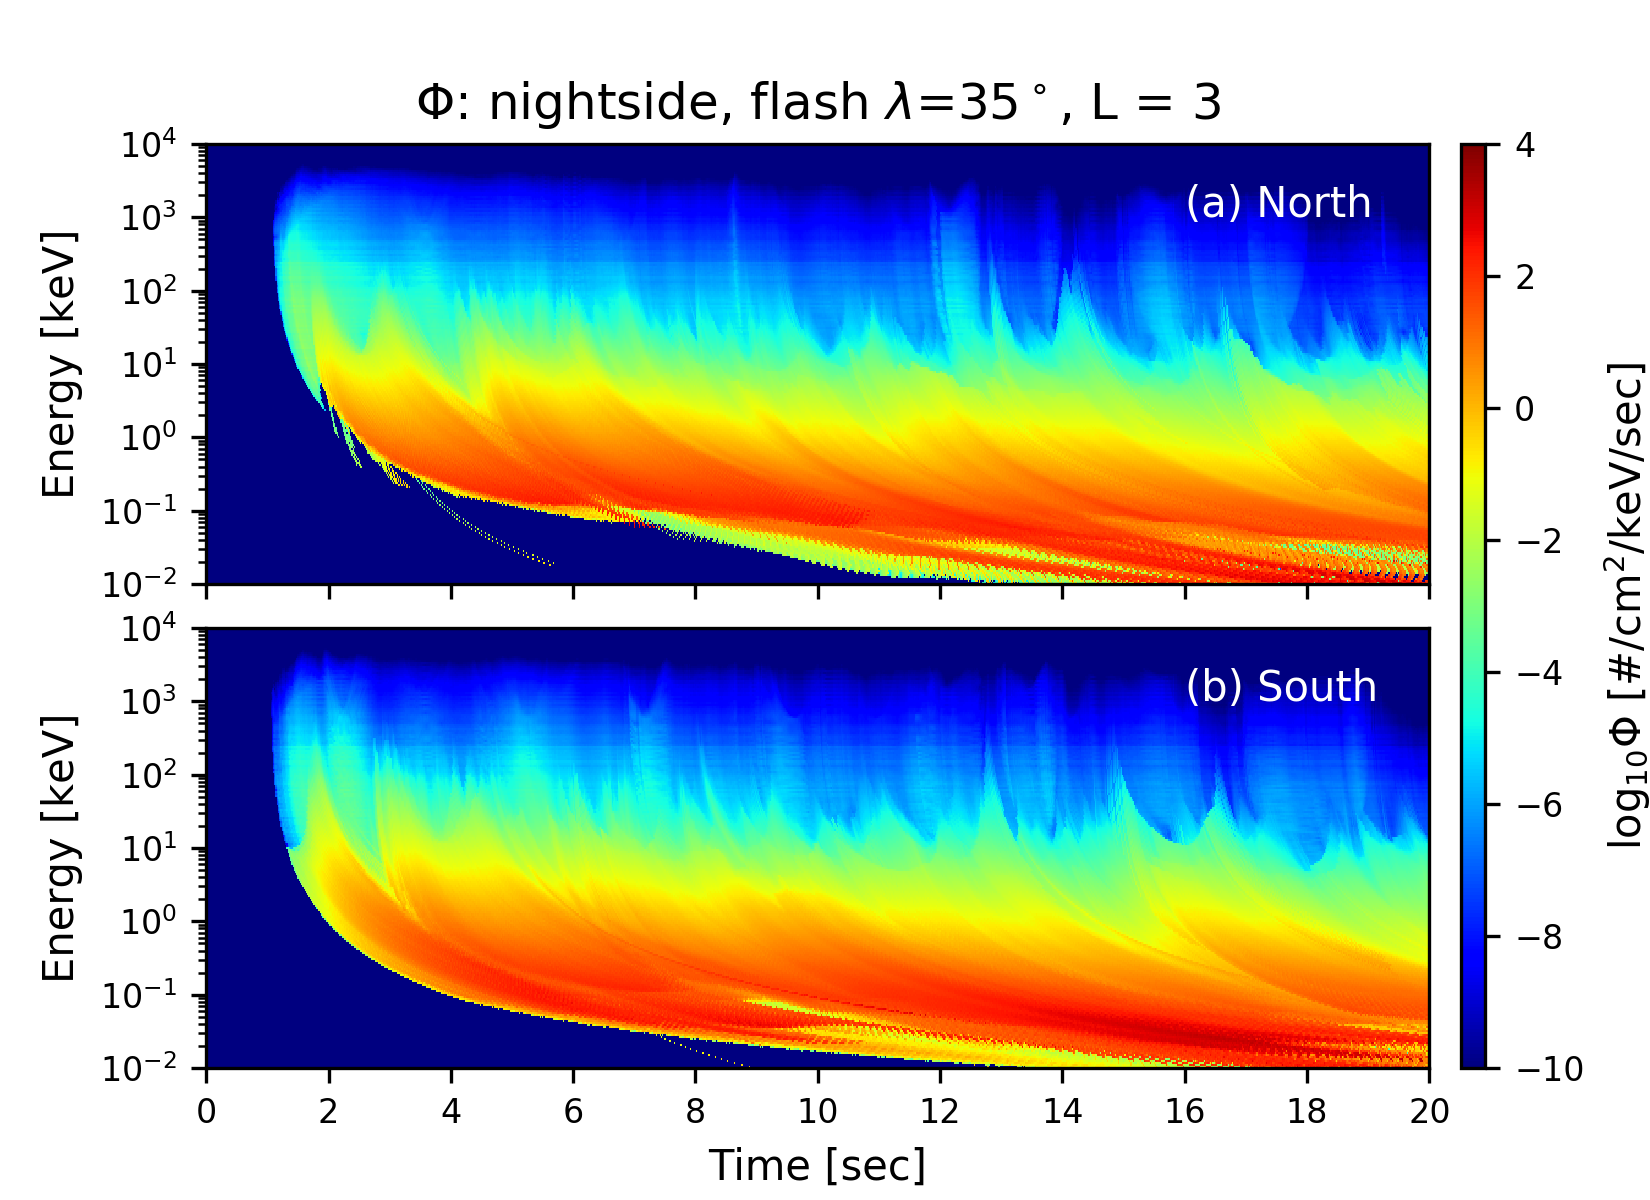
\includegraphics{figures/phi_E-t_spectra.png}
\caption[Precipitating flux density E-t spectra for $\lambda_s=35^\circ$ and L=3]{Precipitating flux density $\Phi(E,t)$ along a fieldine with L=3, for a 10 kA flash at $\lambda_s=35^\circ$ latitude, through a nightside ionosphere at \kp{}=0. Scattering is centered directly over the input flash longitude, within a width of $\pm0.25^\circ.$}
\label{fig:phi_E-t_spectra}
\end{center}
\end{figure}

Equation \eqref{eqn:convolution} is evaluated analytically using a linear expansion of $G(E,t,\alpha)$ about $\alpha = \alpha_{lc}$ (\cite{Bortnik2005}, Figure 5.8, section d).

%The resulting convolution gives a perturbed distribution of pitch angles for each energy band $f_\mathrm{p}(E,t,\alpha)$, a portion of which is within the loss cone. To convert the loss-cone pitch angle distribution to a number (or energy) electron flux density $\Phi_\mathrm{p}(E,t,\alpha)$, we apply the formula from \cite{Chang1983}:
%
%\begin{equation}
%\Phi_\mathrm{p}(E,t,\alpha) = \frac{f_\mathrm{p}(E,t,\alpha)v^2}{m \gamma^3}
%\end{equation} 
%
%where $v$, $\gamma$, and $m$ are the velocity, Lorentz correction factor, and mass of a particle. 
Total fluxes are derived by integrating over the loss cone solid angle, again following \cite{Bortnik2005}, including a $\sin^{-2}\alpha_{lc}$ term to account for fieldline focusing, and $\cos\alpha$ to select the plane perpendicular to $B_0$:

\begin{eqnarray}
\Phi(E,t)& = &\frac{1}{\sin^2\alpha_{lc}}\int_0^{2\pi}\int_0^{\alpha_{lc}}\Phi_\mathrm{p}(E,t,\alpha) \cos\alpha \sin\alpha\,d\alpha\,d\phi \\
&=& \frac{1}{\sin^2\alpha_{lc}} \int_0^{\alpha_{lc}}\Phi_\mathrm{p}(E,t,\alpha) \sin 2\alpha\,d\alpha
\label{eqn:phi}
\end{eqnarray}

Figure \ref{fig:phi_E-t_spectra} shows an example $\Phi(E,t)$ matrix, as calculated with a 10-kA flash at $\lambda_s=35^\circ$, for L=3.


Finally, number flux N and energy flux Q can be calculated by integrating over a desired energy band of interest ($E_1, E_2$):

\begin{eqnarray}
N(t) &=& \int_{E_1}^{E_2} \Phi(E,t)\,dE \\
Q(t) &=& \int_{E_1}^{E_2} E \Phi(E,t)\,dE
\end{eqnarray}



\section{LEP stencils and the behavior of a single flash}
\label{section:lep_stencils}
Having developed a method of computing the precipitating electron energy-time spectrum along a single fieldline, we can compute the global precipitation flux due to terrestrial lightning, using a similar ``stencil'' structure as in Chapter \ref{chapter:power}. We then sum over the time axis to compute the electron flux density in equation \eqref{eqn:phi} for each flash, repeating the calculation for a grid of output L-shells and longitudes, for an array of input latitudes, MLT, and \kp{}.

Table \ref{tab:stencil_params} lists the various parameters used in the stencil simulation. The collection of guide rays are the same as those in chapter \ref{chapter:power}.


\begin{table}[t]
\caption{Stencil Simulation Parameters}
\begin{center}

\begin{tabular}{c|c}
Grid and Interpolation Parameters: \\
\hline \hline
Fine-scale Frequencies & 50 \\
Output L-shell range & 1.2 - 8 \\
Output L-shell spacing & 0.2 \\
Output longitude offsets & \{0, 0.5, 1, 1.5, 2, 5, 10, 20\} \\
Threshold distance from flash & 1000 km \\
 & \\
Resonant Interaction Parameters: \\
\hline \hline
Fieldline latitude spacing & 1$^\circ$ \\
Resonant modes & \{ -5 .. 5 \} \\
Energy bands & 256, log-spaced between 10 eV and 10 Mev\end{tabular}
\end{center}
\label{tab:stencil_params}
\end{table}%

After integrating over the time axis, the resulting stencils each have dimensions (lat $\times$ lon $\times$ energy), for both the northern and southern hemispheres. Figure \ref{fig:precip_stencils} shows a set of energy-integrated number flux stencils for a variety of input latitudes and \kp{} for a 10kA, nightside flash. Figure \ref{fig:precip_stencils_day} shows the corresponding stencils for the dayside.

\begin{figure}[]
\begin{center}
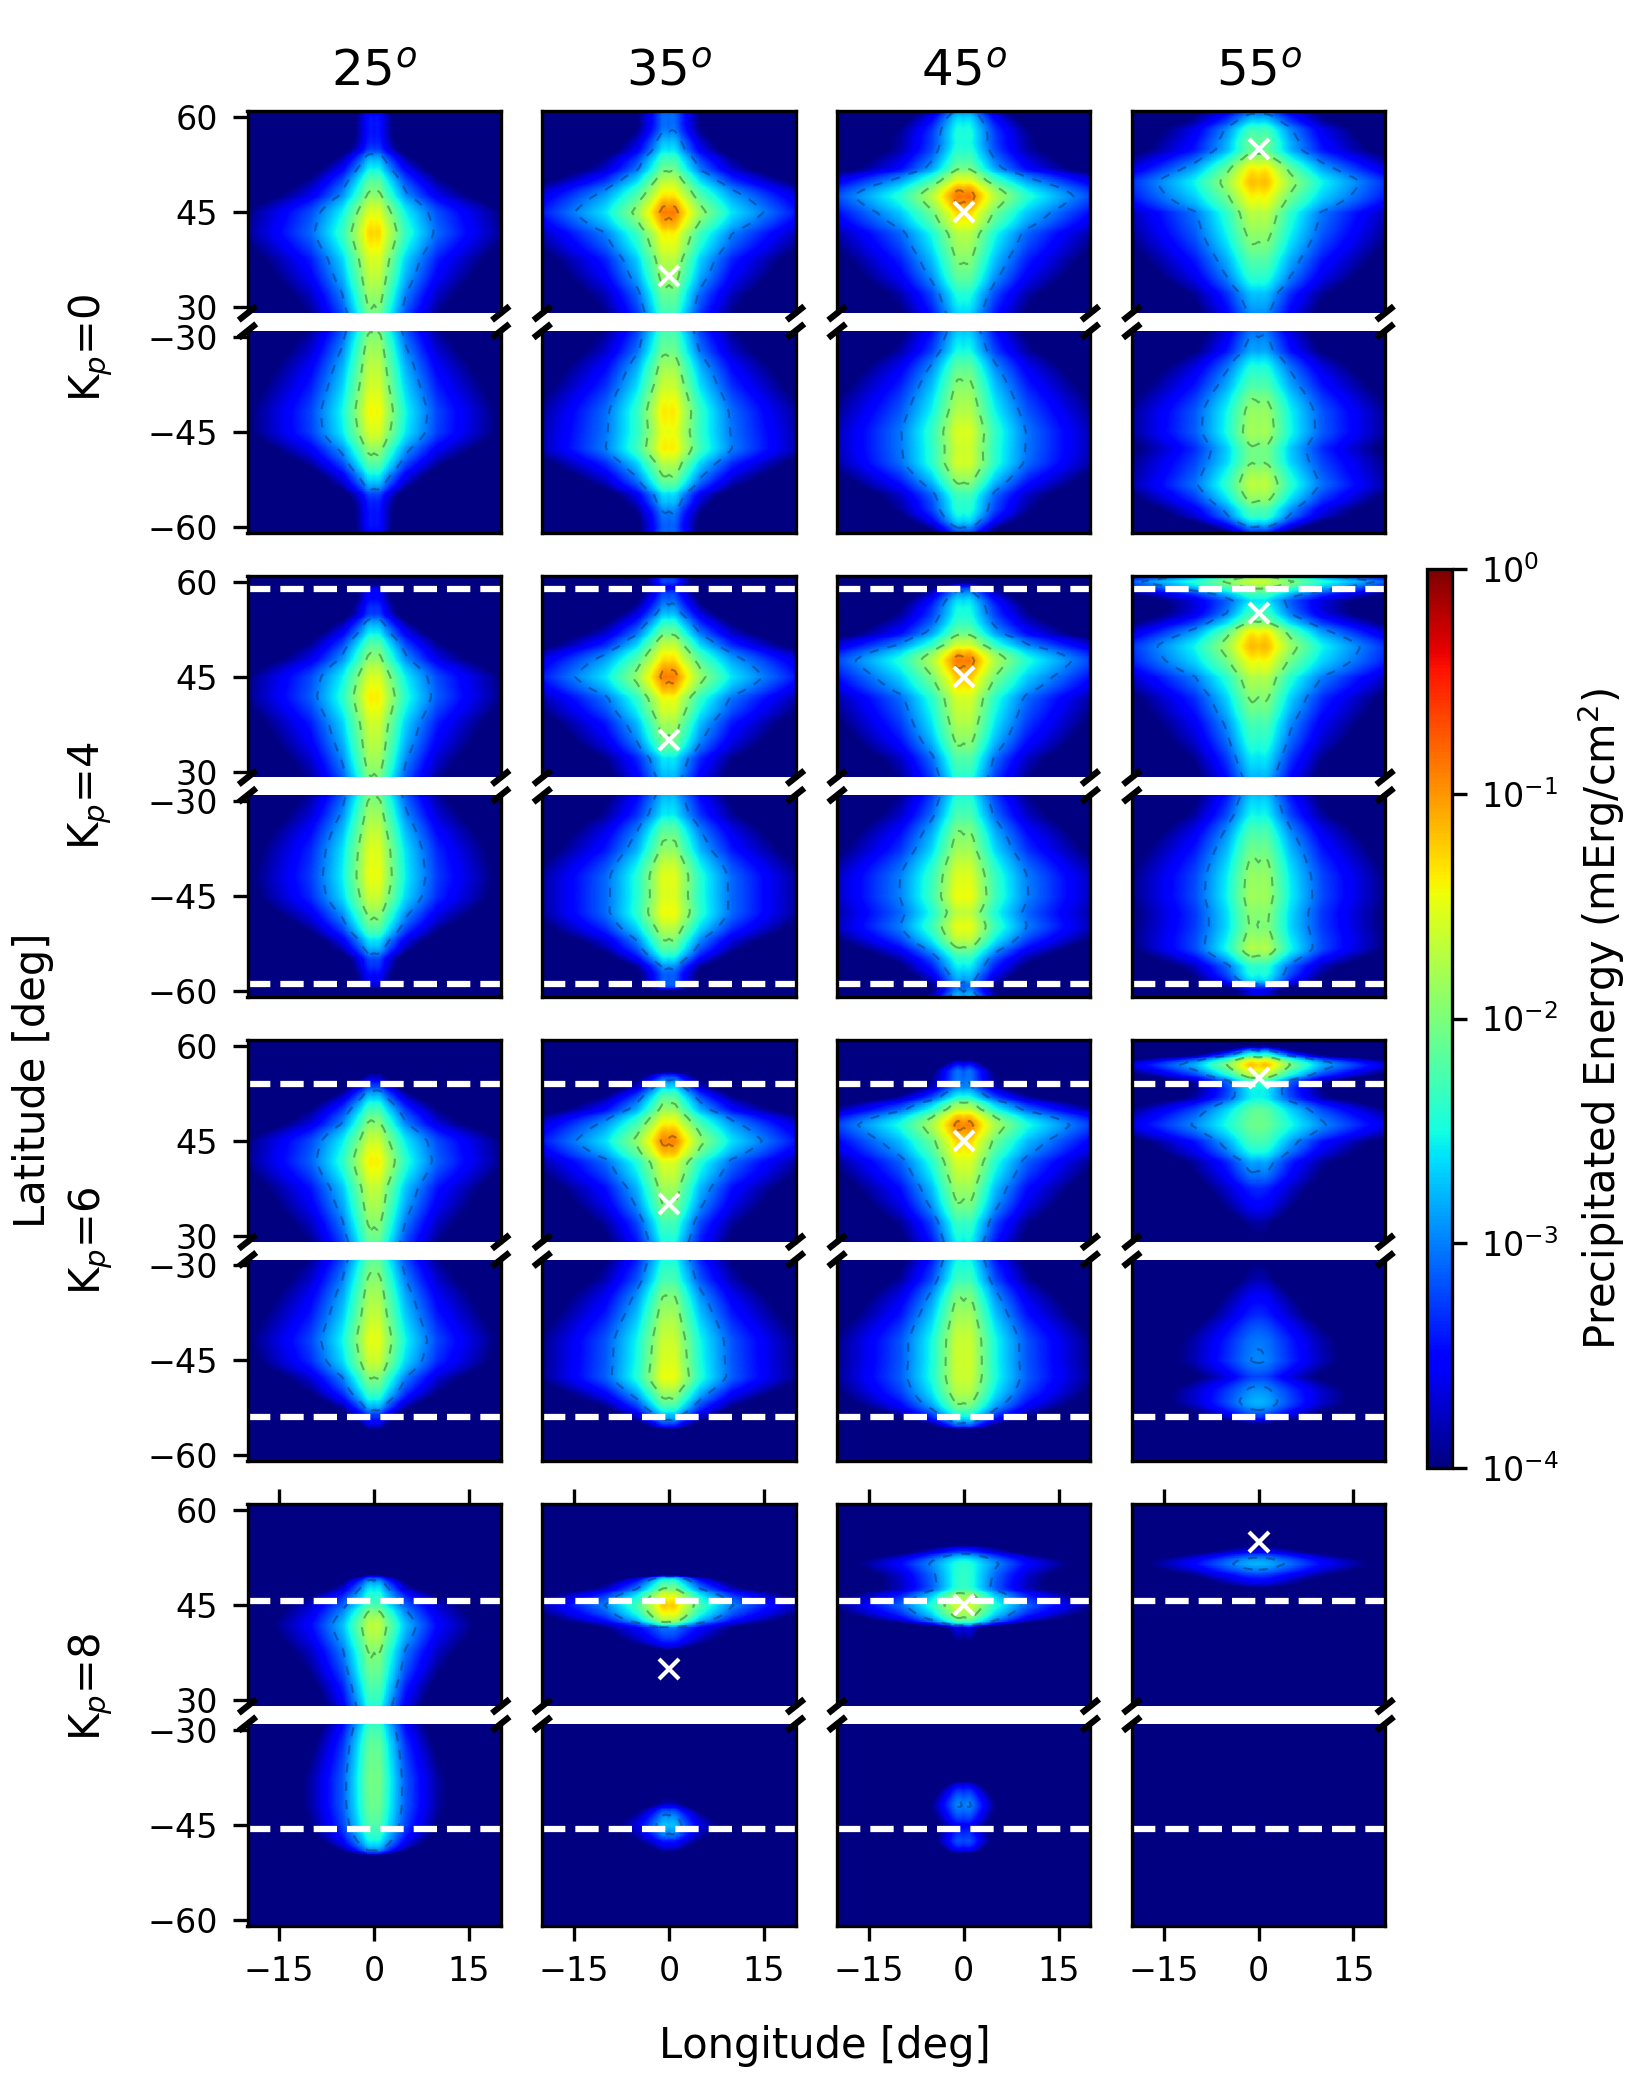
\includegraphics{figures/energy_stencils_nightside_v2.png}
\caption[Precipitating flux density stencils for a range of input latitudes and magnetospheric conditions (nightside)]{Precipitating energy density stencils from a maximally-populated radiation belt model, for a range of flash latitudes and magnetospheric conditions, for a 10 kA nightside flash. The location of the plasmapause is marked with a dashed white line, along the northern and southern hemispheres. The flash location is marked with a white X.}
\label{fig:precip_stencils}
\end{center}
\end{figure}

\begin{figure}[]
\begin{center}
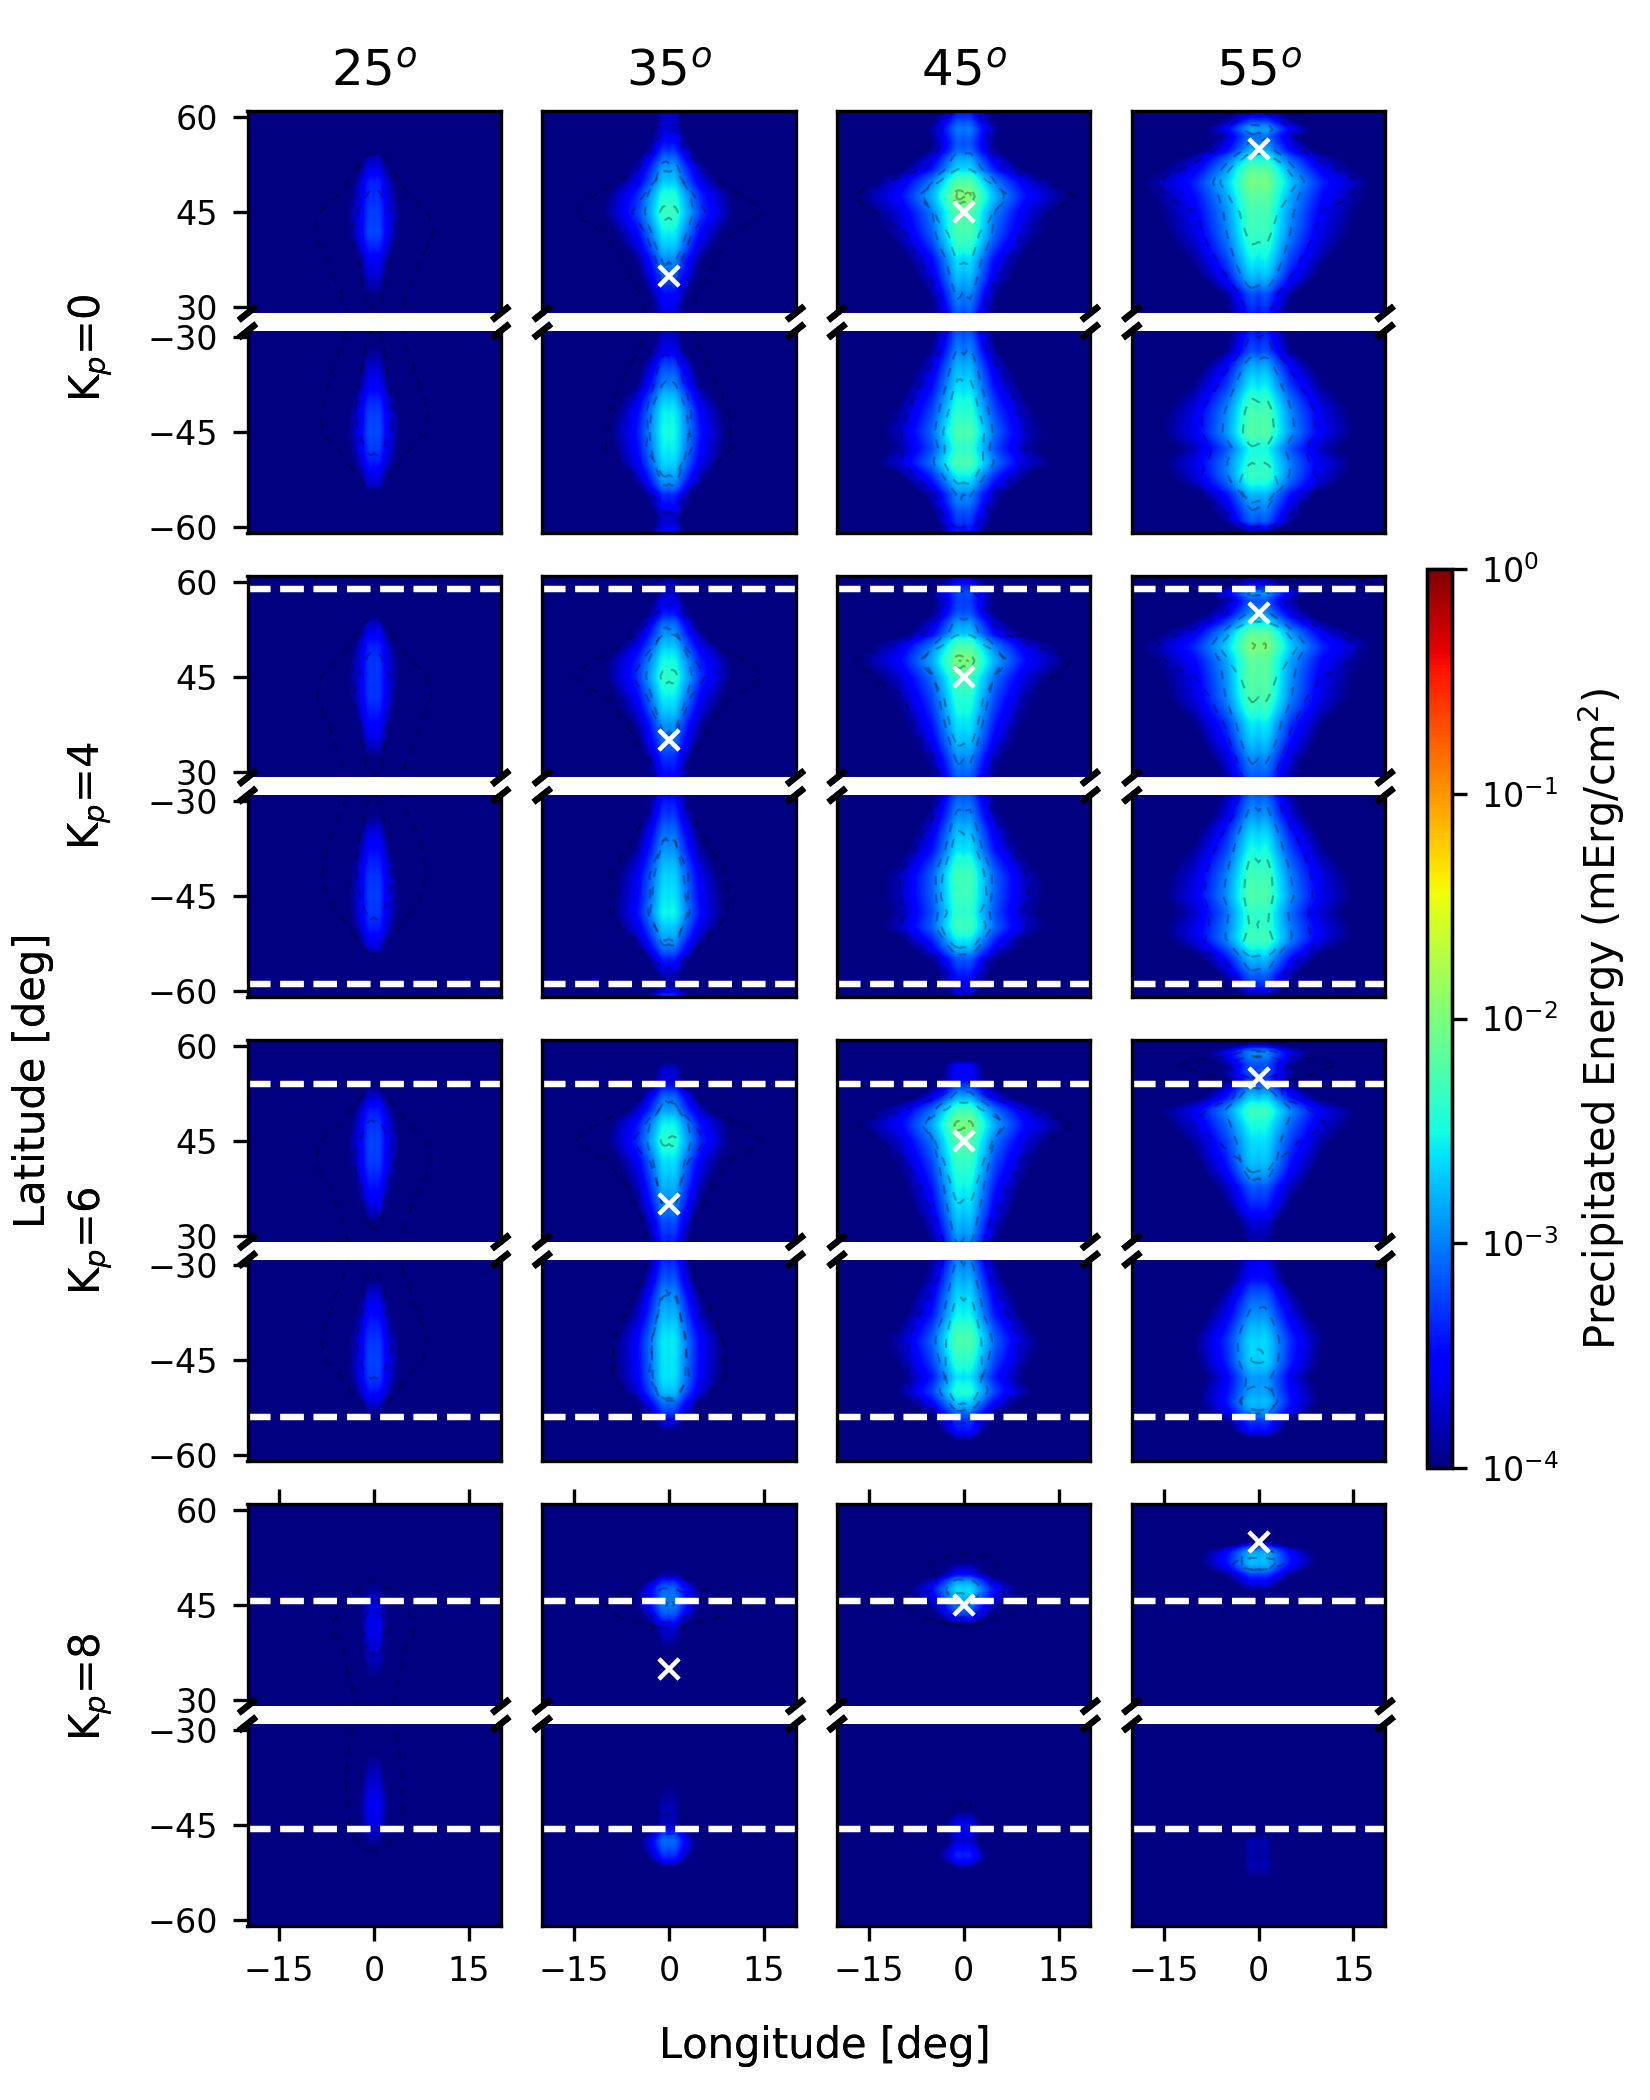
\includegraphics{figures/energy_stencils_dayside_v2.png}
\caption[Precipitating flux density stencils for a range of input latitudes and magnetospheric conditions (dayside)]{Precipitating energy density stencils from a maximally-populated radiation belt model, for a range of flash latitudes and magnetospheric conditions, for a 10 kA dayside flash. The location of the plasmapause is marked with a dashed white line, along the northern and southern hemispheres. The flash location is marked with a white X.}
\label{fig:precip_stencils_day}
\end{center}
\end{figure}

By integrating over latitude and longitude, we can compute the total energy precipitated from a single flash, as shown in Figure \ref{fig:total_energy_per_stencil}. A 10-kA flash precipitates on the order of 1 to 10 kJ on the nightside, and 1 to 1000 J on the dayside.

\begin{figure}[]
\begin{center}
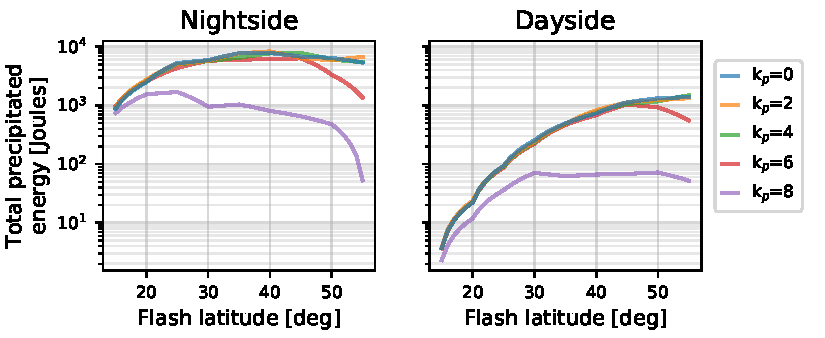
\includegraphics{figures/total_energy_vs_latitude.pdf}
\caption[Total precipitated energy for a single flash]{Area-integrated precipitation for a single 10 kA flash vs flash latitude, for a variety of magnetospheric conditions. Totals include precipitation in both hemispheres.}
\label{fig:total_energy_per_stencil}
\end{center}
\end{figure}

Several trends are apparent in figures \ref{fig:precip_stencils} and \ref{fig:precip_stencils_day}: First, it is apparent that increased \kp{} has little impact on precipitation, up until high activity (\kp{}$ > \sim 6$). We can attribute this to our plasmasphere density model, which is consistent across \kp{} values within the plasmapause. Generally, if a flash is launched within the plasmapause (at a latitude lower than that of the plasmapause), then the rays experience relatively little attenuation due to Landau damping in the cold medium, and reflect back and forth several times. Rays launched outside the plasmapause are attenuated much more quickly. The sharp gradient of the plasmapause constrains energy within the plasmasphere, as indicated by the sharp dropoff of precipitation around the plasmasphere latitude. At the highest values of \kp{}, the plasmapause is brought in to L $\sim$, about 45$^\circ$, at which point substantial energy is launched outside the plasmapause (and quickly damped), or is very strongly deflected by the plasmapause gradient. The effect of the plasmapause is consistent in both the nightside and dayside stencils.

Examining the dayside stencils in Figure \ref{fig:precip_stencils_day}, the increased attenuation of the ionosphere becomes apparent, notably at lower-latitude flashes. The effect of both ionosphere attenuation and of the lower-latitude plasmapause is apparent when looking at the integrated totals in Figure \ref{fig:total_energy_per_stencil}.

Precipitation is not always symmetric between the northern and southern hemispheres. We can attribute any asymmetry in total flux to the relative efficiency of each resonant mode. Higher-order modes (m = $\pm 1$, $\pm 2$...) are symmetric, with the positive calculation resonating with particles moving in one direction, and the negative with particles moving in the opposite. However, the lowest resonant mode (m = 0) interacts only with counterstreaming particles. Accordingly, precipitation is strongest at the same hemisphere as the incident flash.

In both figures \ref{fig:precip_stencils} and \ref{fig:precip_stencils_day}, precipitation is strongest along a $\sim 0.8^\circ$ offset in longitude, which results from the $\sin^2\theta$ term in equation \eqref{eqn:farfield_power_fd}. In this case, $\theta$ represents the elevation angle from the flash to the lower ionosphere (taken to be 100 km), which is maximized at $\theta = 45^\circ$. The result is a central null in radiated energy directly above the flash, and maximal radiated energy offset by 100 km in the longitudinal direction.

An additional point of interest is the ratio of precipitated energy in Figure \ref{fig:total_energy_per_stencil} vs the radiated energy above the ionosphere in Figure \ref{fig:illumination_totals}. Radiation on the order of megajoules will induce precipitation several orders of magnitude lower in energy. 

Finally we can examine the energy spectrum of precipitating electrons, as shown in Figure \ref{fig:stencil_energy_spectrum}. As in the precipitation stencil maps, increasing \kp{} has little effect until very active conditions. The flux is dominated by lower-energy electrons, owing to the stronger scattering of the lowest resonant mode (also visible in Figure \ref{fig:phi_E-t_spectra}).

\begin{figure}[t]
\begin{center}
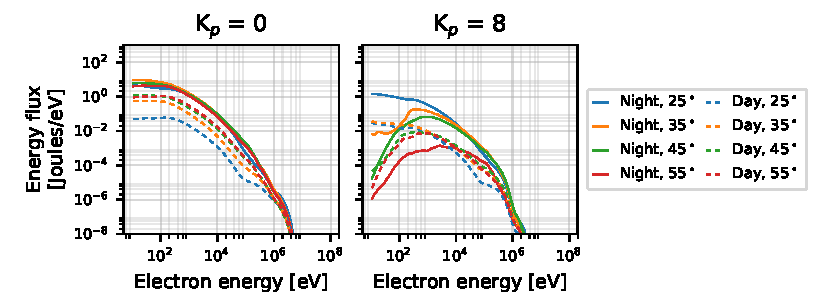
\includegraphics[clip]{figures/stencil_energy_spectrum.pdf}
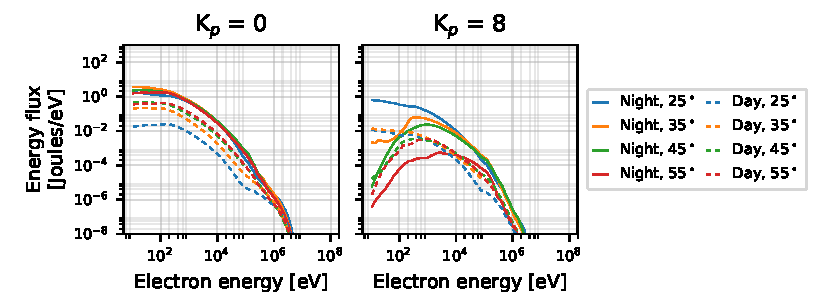
\includegraphics[clip]{figures/stencil_energy_spectrum_AE8MIN_flux_0.pdf}
\caption[Energy spectrum of LEP stencils]{Energy spectrum of precipitating electrons, for \kp{}= 0 and 8, for a range of input latitudes, for day and night. Fluxes are drawn from the AE8MAX population model in the top row, and from the AE8MIN population model in the bottom row.}
\label{fig:stencil_energy_spectrum}
\end{center}
\end{figure}


\section{Coordinate deformation}
The stencils in section \ref{section:lep_stencils} are computed using a dipole magnetic field, and the simplified GCPM model, both to reduce computational complexity and to better generalize to multiple longitudes. However, we can approximate the effect of a more-complex magnetic field model via a coordinate transformation, in which we rotate input coordinates to an equivalent dipole-model coordinate, and perform an inverse operation on the stencil output. On the stencil output, this approximation is justified by noting that trapped electrons are bound to their respective field lines, regardless of model used. Justification on the input side (deforming the input coordinates of a lightning flash) is less-concrete, but still a reasonable assumption. First, experimentation with the raytracer reveals that, given a longitudinally-symmetric plasma density model, rays generally follow the longitude deviation of the magnetic field model. Second, while the IGRF and Dipole models differ greatly in its footprint on the ground (as in Figure \ref{fig:Lshell_example}), within the plasmasphere the two models have reasonable agreement (as in Figure \ref{fig:fieldline_example}).

The \emph{Corrected Geomagnetic Coordinate} (CGM) \citep{Hakura1965} system is especially well-suited for this task. CGM coordinates are defined by fieldline tracing between the IGRF and Dipole models. To transform from geographic to CGM coordinates, we first trace a fieldline using IGRF from the surface, up to its intersection with the geomagnetic equatorial plane. We then follow the dipole model back down to the surface, to get an equivalent dipole-model coordinate. The inverse transformation is accomplished by following the dipole field line back up to the equator, and the IGRF model down to its footprint \citep{Laundal2016}.

Field line tracing is a computationally-intensive task for a coordinate transformation tool. Historically, researchers relied on precomputed lookup tables and interpolation. The Altitude-Adjusted CGM (AACGM) model \citep{Baker1989, Shepherd2014} uses a spherical-harmonic fit to rapidly transform between CGM and MAG coordinates.

\begin{figure}[t]
\begin{center}
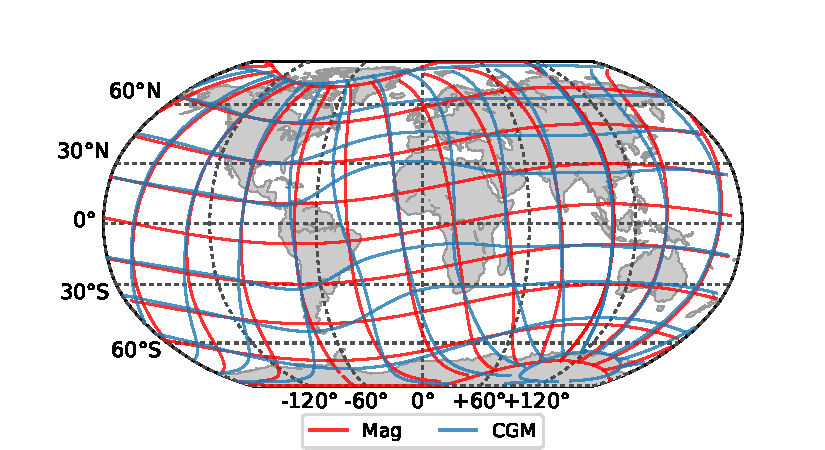
\includegraphics{figures/CGM_globe_comparison.pdf}
\caption[Comparison of Magnetic Dipole (MAG) and Corrected Geomagnetic (CGM) coordinates]{A comparison between Magnetic Dipole (MAG) and Corrected Geomagnetic (CGM) coordinates. Corrected Geomagnetic coordinates are obtained by following a magnetic field line, as defined by IGRF, from an input point to its intersection with the magnetic dipole equator. The CGM latitude and longitude are then obtained by following the dipole field line to its footprint on the Earth's surface. Contours are spaced every $20^\circ$ in geomagnetic latitude, and $30^\circ$ in geomagnetic longitude.}
\label{fig:CGM_globe_comparison}
\end{center}
\end{figure}    

CGM coordinate systems are undefined at some regions near the geomagnetic equator, due to the fact that some IGRF fieldlines may never intersect with it. In these cases, approximate models are often used. \cite{Baker1989} simply omitted geomagnetic latitudes within $\sim 24^\circ$ of the equator from their study; subsequent researchers have performed spline fits and interpolation to further reduce the undefined region.

We use the AACGMv2 algorithm and implementation from \cite{Shepherd2014}, available at \emph{http://superdarn.thayer.dartmouth.edu/aacgm.html}. Figure \ref{fig:CGM_globe_comparison} compares MAG and AACGM contours on a geographic map.

Figure \ref{fig:CGM_vs_MAG_GLD} shows the relative difference between GLD average current density using MAG coordinates only, vs using the AACGM coordinate transform.



\begin{figure}[]
\begin{center}
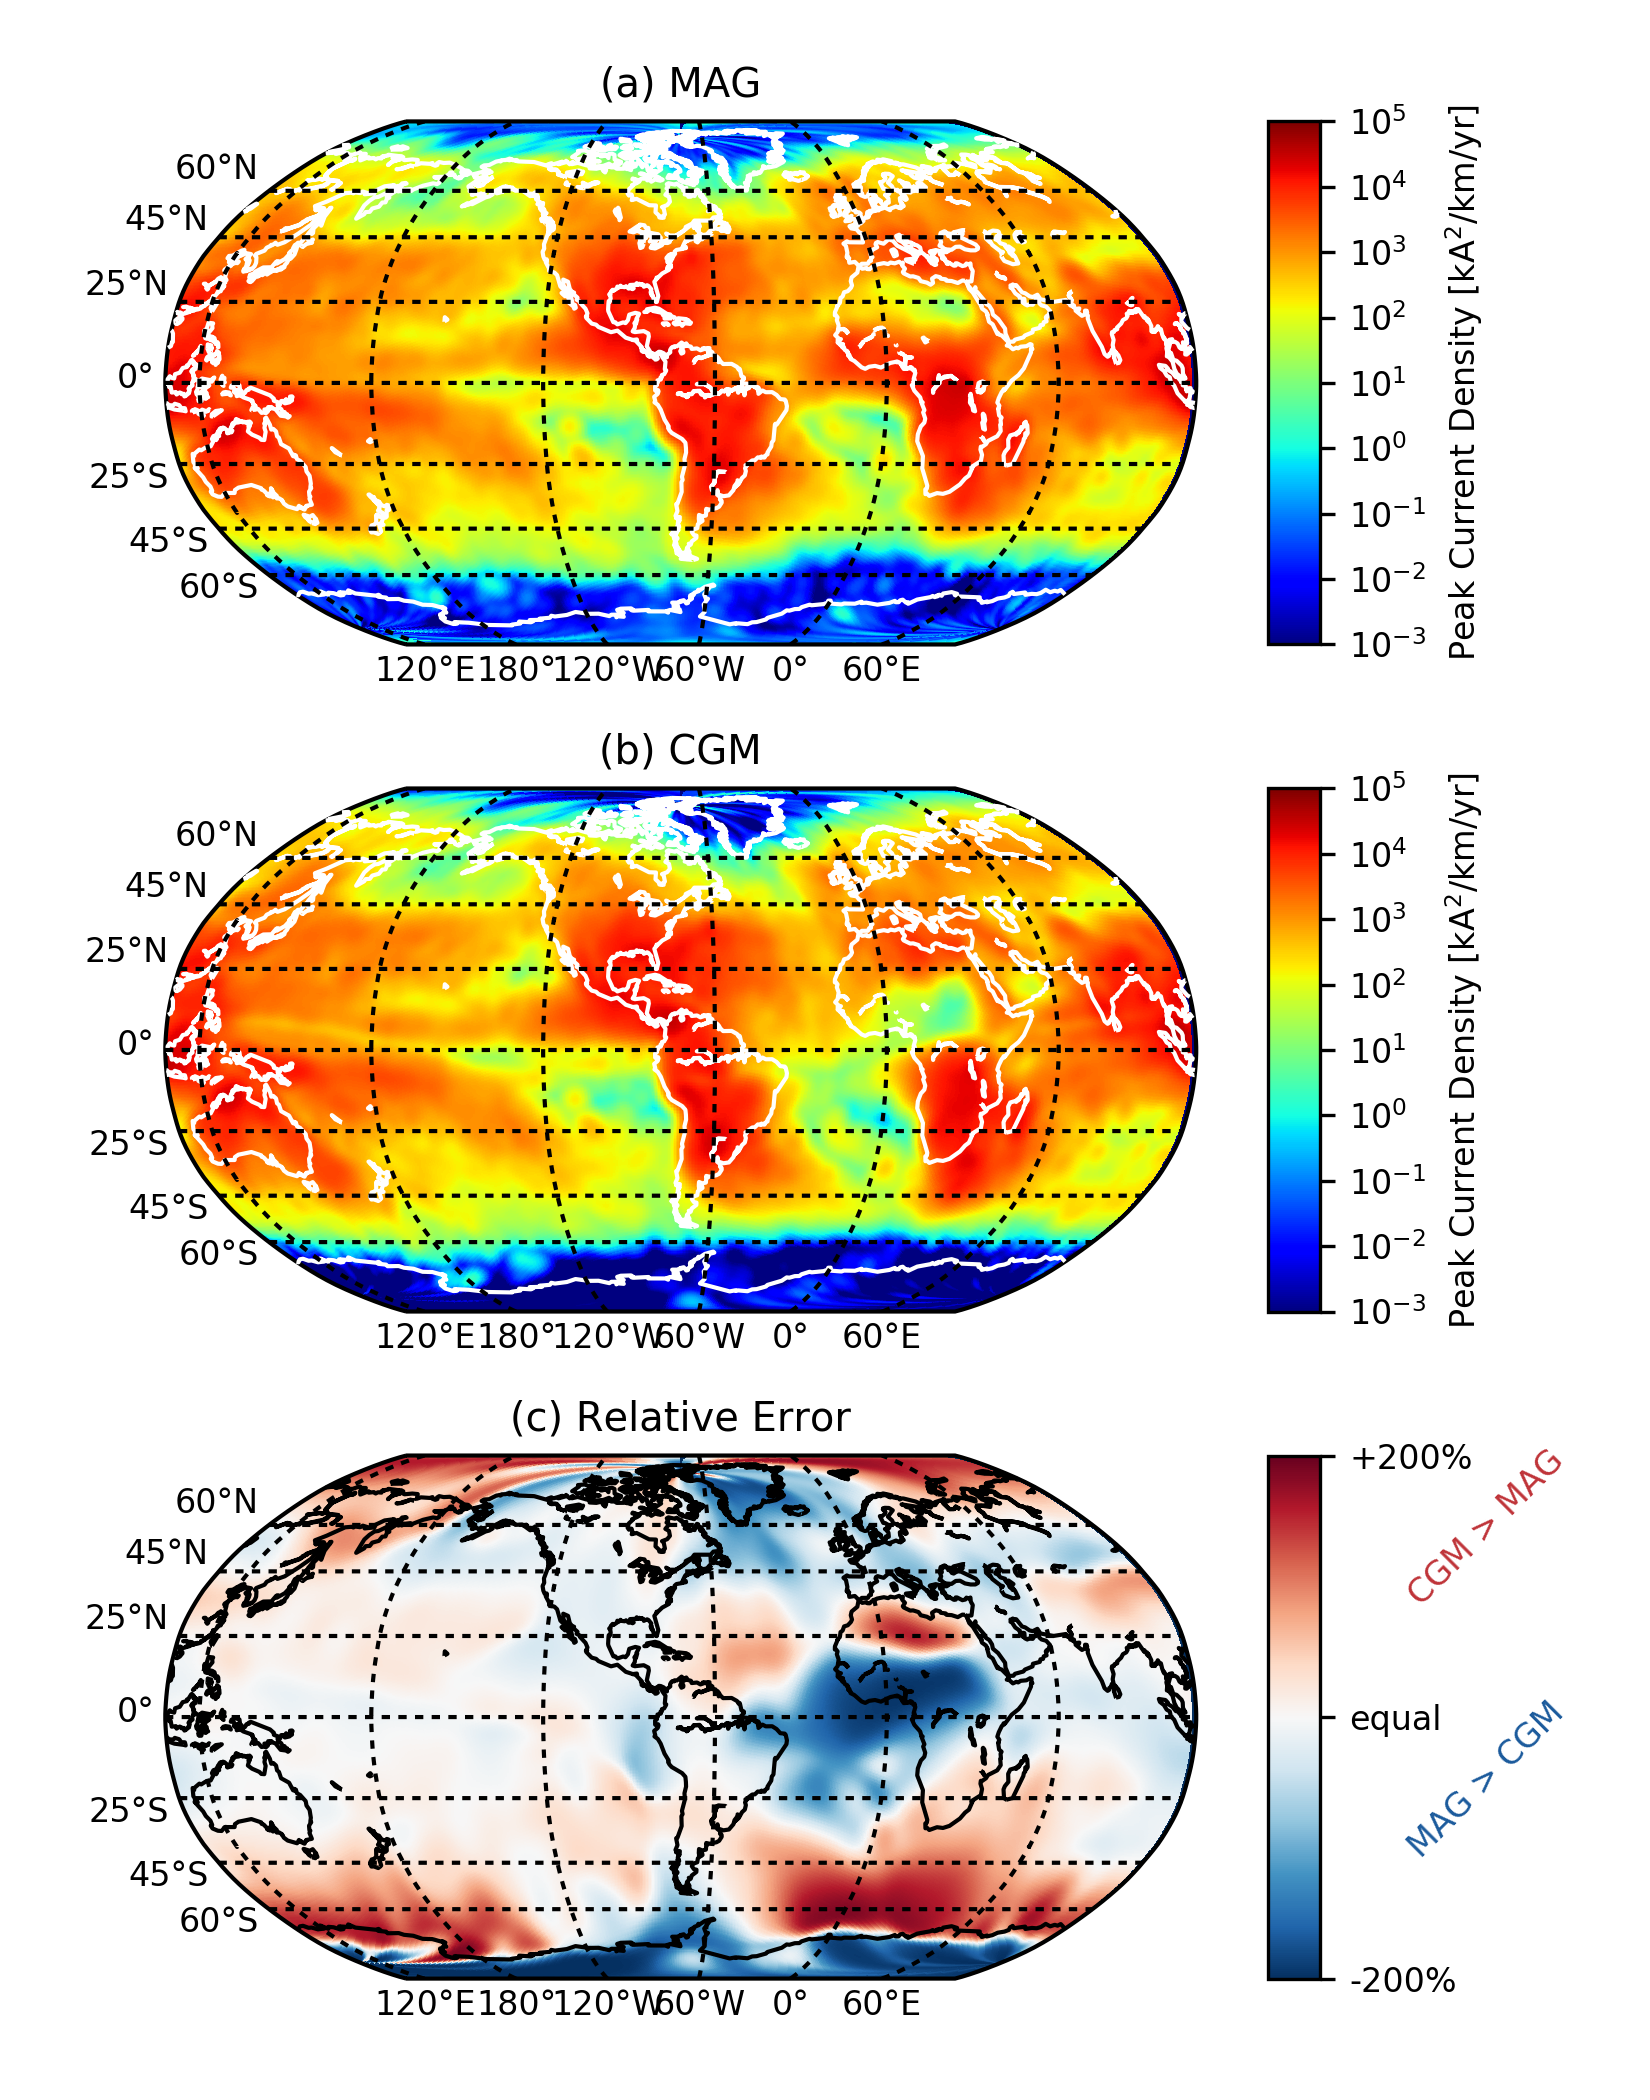
\includegraphics{figures/GLD_CGM_vs_MAG_comparison.png}
\caption[GLD average peak current density, adjusted using AACGM coordinates]{Average lightning activity, weighted by peak current intensity, as measured by the GLD360 dataset. Data is averaged from August 2014 through July 2017. (a) the GLD360 data, in geographic coordinates. (b) the GLD360 data, shifted to its equivalent coordinates using the AACGM coordinate transform. (c) the relative error between the two coordinate frames.}
\label{fig:CGM_vs_MAG_GLD}
\end{center}
\end{figure}


% Our study already excludes these latitudes on the basis that below $\sim 20^\circ$ geomagnetic latitude, field lines do not exit the ionosphere at their apex.


\section{Global and Seasonal Energy Fluxes}

Having computed the precipitation for a single flash across a variety of input parameters, we can examine global energy deposition by shifting, scaling, and summing the LEP stenciles according to the GLD360 lightning dataset. The resulting electron precipitation is heavily dependent on the population of radiation belt electrons; rather than leverage historical data, we provide two estimates, using the AE8 model for maximal and minimal filling, in effort to determine the upper and lower bounds on precipitation. 

LEP stencils are computed using the parameters in table \ref{tab:stencil_params}. Stencils are computed for canonical 10 kA flashes, in 5$^\circ$ steps in latitude, between 15$^\circ$ and 55$^\circ$, for dayside and nightside (MLT = 12 and 0 respectively), for an array of \kp{} = \{0, 2, 4, 6, 8\}. The resulting stencils are then interpolated onto a fixed 0.5$^\circ$x0.5$^\circ$ grid in geomagnetic latitude and longitude, and for all valid values of \kp{} (0 - 9 in $\sim$ 0.3 steps). Noting the relatively quick transition at the day/night terminator, we bin each flash in the GLD360 dataset into dayside or nightside. The 256 energy bands are summed into 64 sub-bands to reduce memory requirements. 

Figure \ref{fig:global_precip_map_max_min} shows the global average energy precipitation resulting from LEP, for maximum and minimum conditions. Precipitation is integrated over the energy band of interest (10 eV - 10 MeV), and averaged over a three year period between August 2014 and July 2017. We use historical data for \kp{}, which is reported in three-hour segments.

The pitch-angle scattering model scales linearly with respect to wave amplitude, and therefore scales quadratically with respect to flash peak current. To account for arbitrary peak current values, we scale the resulting precipitation stencils accordingly:

\begin{equation}
\phi(I) = \phi(I_{ref})\frac{I^2}{I_{ref}^2} 
\end{equation}

The two sources of stochasticity in our model are 1) the location and intensity of lightning, and 2) the value of \kp{}. Lightning activity and \kp{} are generally uncorrelated, as \kp{} is driven by activity within the magnetosphere, and lightning activity by terrestrial weather patterns. As shown in figures \ref{fig:precip_stencils} and \ref{fig:precip_stencils_day}, fluctuations in \kp{} have little effect on our precipitation model in most situations (\kp{}$ < 6$). Unexplored in this work, however, is the correlation between radiation belt filling conditions and \kp{}; e.g., radiation belt filling events generally occur alongside geomagnetically-active conditions, in which \kp{} will be high.

\begin{figure}[]
\begin{center}
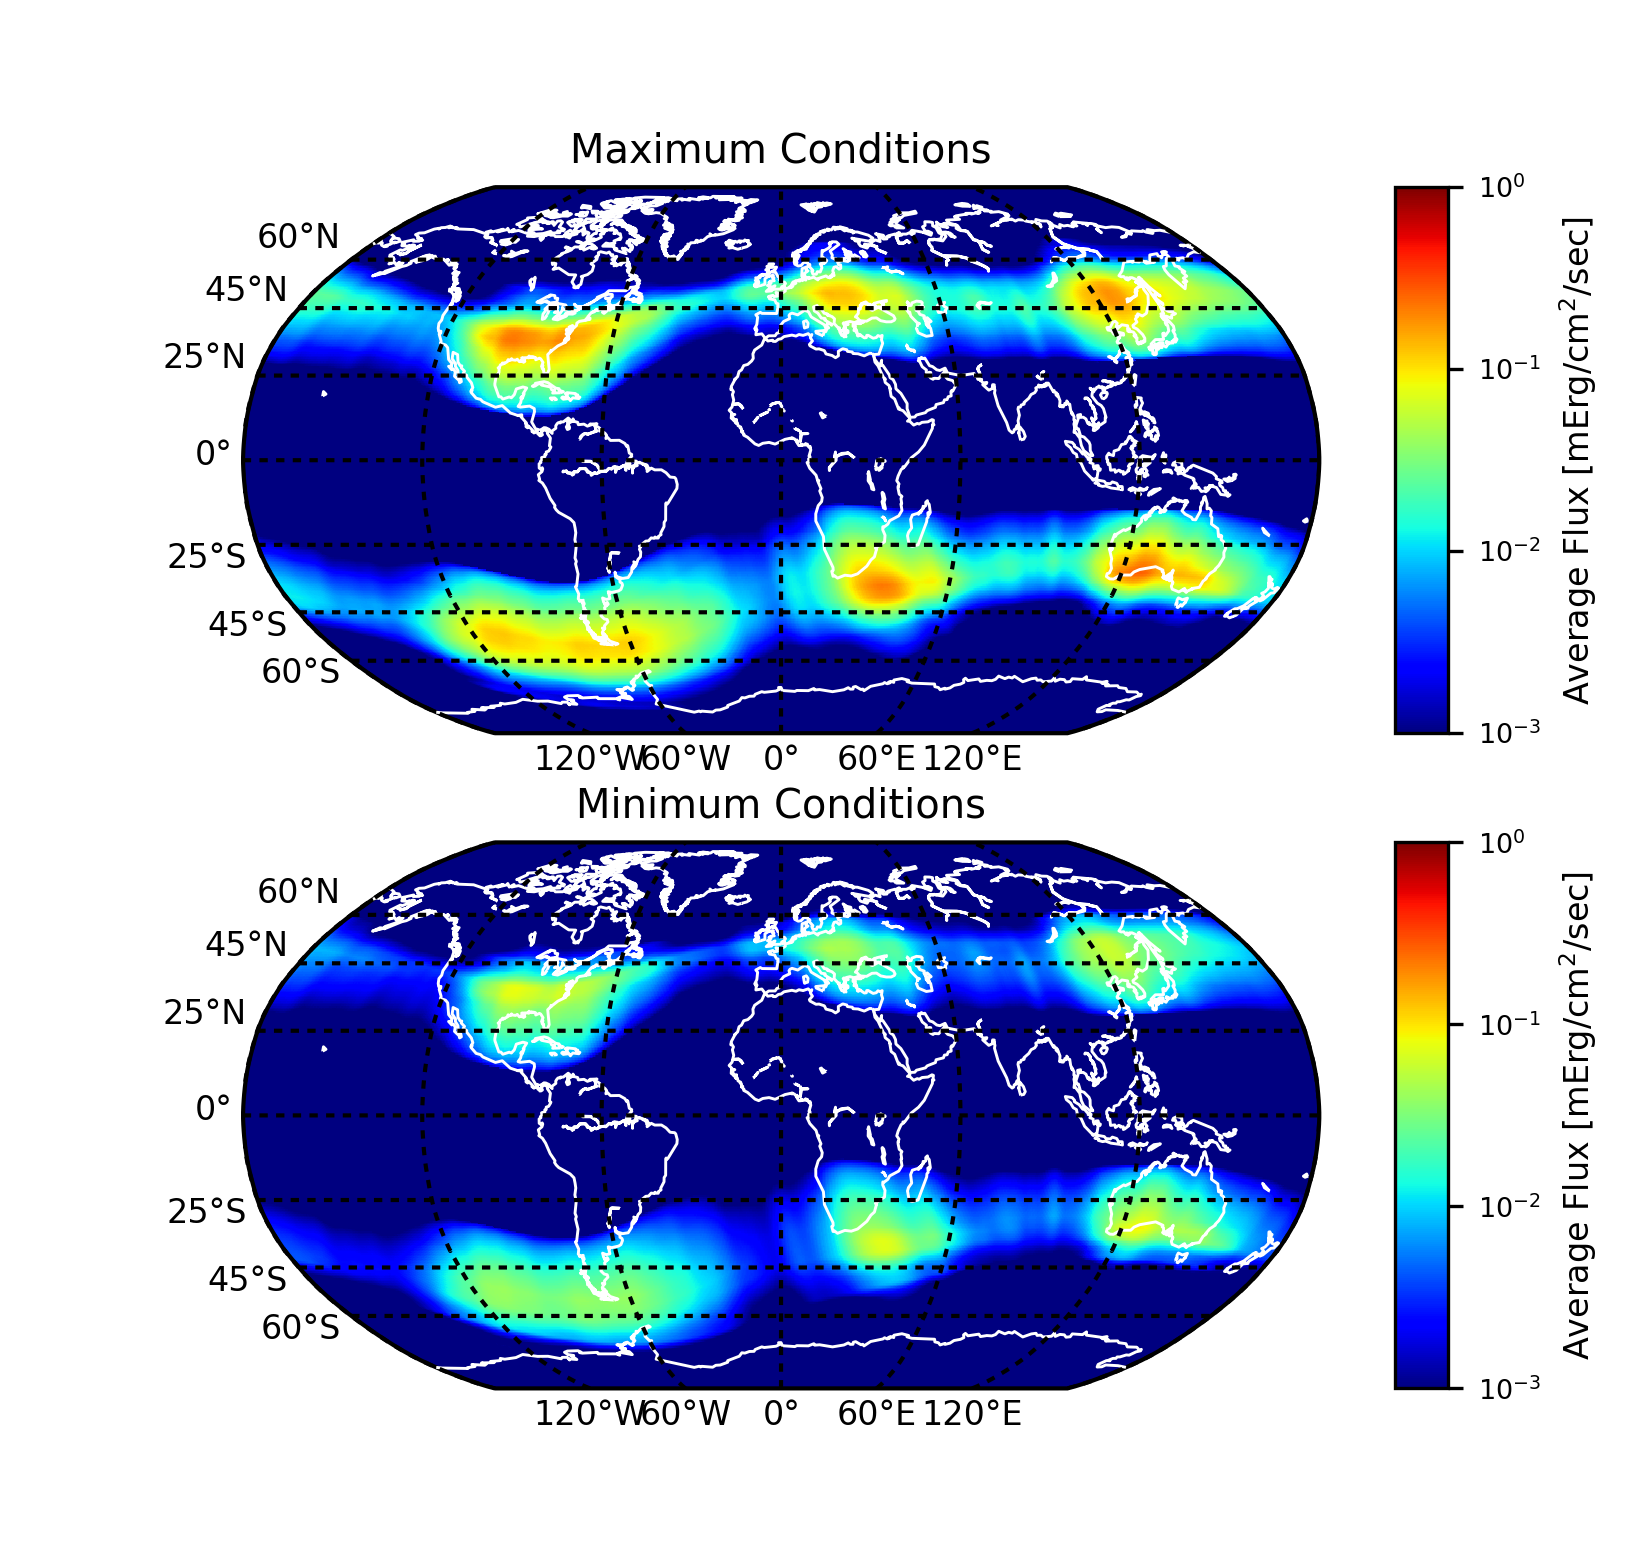
\includegraphics{figures/global_precip_map_max_min.png}
\caption[Global energy deposition ``hot spots'' for maximal and minimal radiation belt populations]{Time-averaged energetic electron precipitation ``hot spots'', for the GLD360 dataset, between August 2014 and July 2017. Total energy is shown, integrated between 10 eV and 10 MeV. }
\label{fig:global_precip_map_max_min}
\end{center}
\end{figure}

By integrating over latitude and longitude, rather than time, we can examine any seasonal trends which may be present. Figure \ref{fig:seasonal_precip_rates_global} shows the global energy flux in kilowatts, across the globe, as a function of time, for maximal and minimal filling conditions. The global energy deposition rate shows very weak seasonal dependence, and can range from a few kilowatts to several megawatts. The disperse energy deposition rate suggests that LEP is not a prominent driver of energy in the upper atmosphere. However, sporadic energy deposition due to LEP is measurable by sub-ionosphere VLF remote sensing \citep{Inan1990, Johnson1999, Cotts2011}, and may still be capable of inducing turbulence in the upper ionosphere, either by precipitating particles or the interaction of the upgoing whistler wave \citep{Berthelier2008}.

The lack of seasonal dependence, however, suggests that LEP can provide a constant, year-round loss mechanism for radiation belt electrons, especially when considering that radiation belt electrons can drift in longitude around the Earth, on timescales of minutes to days \citep{Walt1994}, and can thereby interact with lightning activity across the globe.

\begin{figure}[ht]
\begin{center}
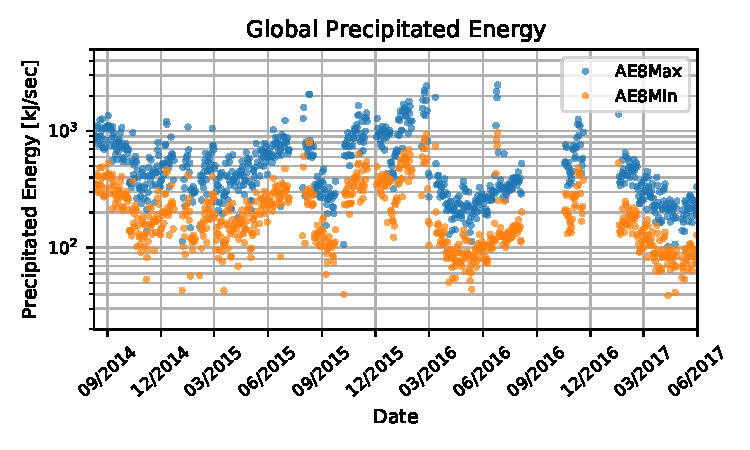
\includegraphics{figures/seasonal_precip_rates_global.pdf}
\caption[Global energy deposition due to LEP]{Global average energy deposition due to LEP. Precipitation is integrated across the globe, for energetic electrons between 10 eV and 10 MeV.}
\label{fig:seasonal_precip_rates_global}
\end{center}
\end{figure}
\begin{figure}[h]
\begin{center}
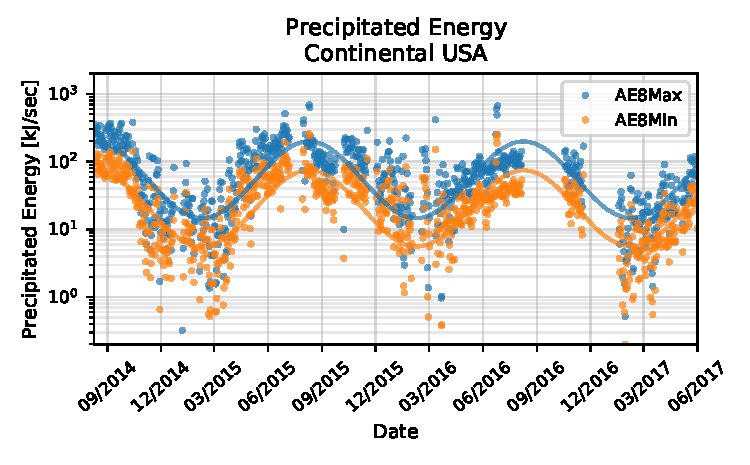
\includegraphics{figures/seasonal_precip_rates_US_only.pdf}
\caption[Global energy deposition due to LEP over the continental United States]{Average energy deposition due to LEP over the continental United States (20$^\circ$ to 50$^\circ$ geomagnetic latitude, -50$^\circ$ to +10$^\circ$ geomagnetic longitude). Seasonal variation is much more apparent than in the global integration (Figure \ref{fig:seasonal_precip_rates_global}).}
\label{fig:seasonal_precip_rates_US_only}
\end{center}
\end{figure}

While total global lightning activity is relatively constant, regional lightning is a highly seasonal phenomenon. We can integrate the energetic electron precipitation over the continental United States, to explore seasonal dependence on a finer scale, such as in \cite{Gemelos2009}. Figure \ref{fig:seasonal_precip_rates_US_only} shows the total energy precipitation between 20$^\circ$ - 50$^\circ$ in geomagnetic latitude, and -50$^\circ$ to +10$^\circ$ in geomagnetic longitude (approximately over the continental United States). Narrowing our observation window reveals a much greater seasonal variation, peaking in the summer months, and reaching a minimum in December and January.



\section{Lifetime Estimates}
The previous section examined the energy deposition into the ionosphere due to LEP. Next, we consider the relative effect of LEP as a loss mechanism from the populated radiation belts.

Our precipitation model is linearly proportional to the current population of electrons along a given magnetic fieldline, which results in an exponential loss function, parameterized by a time constant $\tau$:

\begin{eqnarray}
\frac{dN}{dt} & \propto & N \\
\therefore N(t) & = & N_0 \exp{-t/\tau} \\
\frac{dN}{dt} & = & -\frac{N_0}{\tau}\exp{-t/\tau} \\
& = & -\frac{N(t)}{\tau} \\
\tau & = & \frac{N(t=t_0)}{dN/dt\rvert_{t0}}
\label{eqn:tau}
\end{eqnarray}

Once summed over the GLD360 dataset, our model delivers electron losses impinging on a cross-sectional area at 100 km, with units [$\#$/cm$^2$/eV/sec]. To compute the percentage loss, we must determine the number of electrons (per energy) which occupy the fieldline above the same cross-sectional area, resulting in $\tau \sim sec$.

The total electrons along a given fieldline above a cm$^2$ ionosphere patch is computed by integrating the (energy) differential, omnidirectional equatorial flux, such as from the AE8 model. As in the precipitation code, we ascribe a sinusoidal pitch-angle distribution (e.g., Figure \ref{fig:pitchangledistributions}) to the electrons in the omnidirectional flux value. 

The AE8 energy-differential, omnidirectional flux models have units J $\sim$ [$\#$/cm$^2$/sec/ev], which represent the total flux of electrons through a cross-sectional area at the equator, per unit energy. We use a change of variables and integrate over the sinusoidal pitch-angle distribution P(L, $\alpha$), using the relationship in equation \eqref{eqn:bounce_time} to relate an electron's bounce time $\tau_b$ to it's pitch angle $\alpha$ and total kinetic energy $E$.

\begin{equation}
  P(L,\alpha)=\begin{cases}
    \bigfrac{1}{1 - 2\alpha_{lc}/\pi}\sin{\bigfrac{\alpha - \alpha_{lc}}{1 - 2\alpha_{lc}/\pi}}, & \text{$\alpha_{lc} < \alpha < \pi - \alpha_{lc}$}. \unit{rad^{-1}}\\
    0, & \text{otherwise}.
  \end{cases}
\end{equation}


\begin{equation}
 % There's more to this -- I'm not showing the whole integrand after the change of variables and addition of the pitch-angle distribution
N_{0,equator} = \int_0^{\pi/2} J(E)P(L,\alpha) \tau_b(L, \alpha)\,\sin{\alpha}\,\cos{\alpha}\,d\alpha \unit{\#/cm^2/eV}
\end{equation}

We then convert the integrated value $N_0$ from an equatorial cross-sectional area to an equivalent cross-sectional area at the ionosphere, using a ``crunch'' term $C_b$ according to the constricting dipole magnetic field:

\begin{eqnarray}
\epsilon_m &= & \frac{1}{L}(R_E + H_{iono})/R_E \\
C_b & = & \sqrt{1 + 3(1 - \epsilon_m)} / \epsilon_m^3 \\ 
N_{0, iono} &=& C_b\,N_{0, equator} \unit{\#/cm^2/eV}
\label{eqn:fieldline_density}
\end{eqnarray}

In order to examine the effectiveness of LEP across all energies, and avoid numerical issues where the AE8 model values are small, we compute an additional set of stencils, using a uniform radiation belt population, by setting $J(E) = 1$ [1/cm$^2$/sec/ev].  Figure \ref{fig:stencil_energy_spectrum_flat_distribution} shows the precipitated energy distribution from a flat radiation belt population, in the same format as Figure \ref{fig:stencil_energy_spectrum}. The bimodal peaks resulting from the multiple resonant interaction modes are more-readily visible, without the additional loss due to reduced radiation belt populations at higher energies.

\begin{figure}[]
\begin{center}
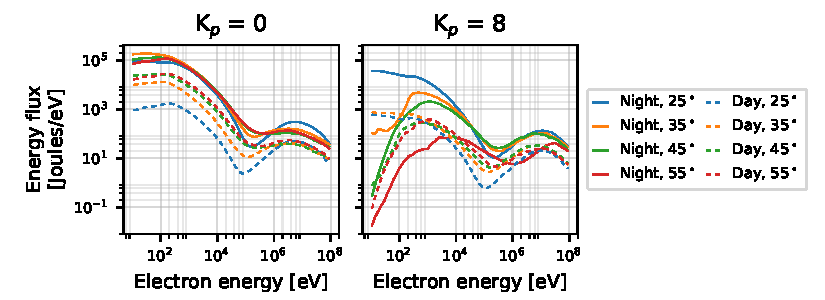
\includegraphics{figures/stencil_energy_spectrum_flat_distribution.pdf}
\caption[Energy spectrum of LEP stencils, drawn from a uniform radiation belt population]{Energy spectrum of precipitating electrons, for \kp{}= 0 and 8, for a range of input latitudes, for day and night, from a uniform (differential flux = 1/cm$^2$/sec/eV) fieldline population.}
\label{fig:stencil_energy_spectrum_flat_distribution}
\end{center}
\end{figure}

We then compute an equivalent precipitation map using the GLD360 dataset, and the flat-distribution stencils. We average the resulting precipitation over all latitudes to obtain a typical flux estimate. The loss timescale, $\tau$, is then obtained using equation \eqref{eqn:tau}, with the fieldline population $N$ computed using equation \eqref{eqn:fieldline_density}, and the loss rate $dN/dt$ given by the global average precipitation estimate, both using the flat distribution for $J$.

Figure \ref{fig:electron_lifetimes} shows the estimated lifetime for radiation belt electrons, subjected solely to LEP-induced losses, versus electron energy and fieldline. Two prominent results are apparent in Figure \ref{fig:electron_lifetimes}: First, we see two enhancement regions, centered at lower energies ($\sim$100 eV), and at higher energies ($\sim$ 10 MeV). We can attribute this bimodal pattern to the preferential energy bands of each resonant mode, as in Figure \ref{fig:stencil_energy_spectrum_flat_distribution}. Interestingly, our model shows a null in precipitation effectiveness in the band between 100 keV and 1 MeV; this band has generally been thought to be the dominant precipitation region (for example, the analysis of a single LEP event in \cite{Voss1998} shows a precipitation spectrum between $\sim$ 100  -- 300 keV. The instrument used, SEEP, measured fluxes binned into 8 energy channels between 2 keV and 10 MeV.) . Second, LEP is only an effective loss mechanism for inner belt and slot-region fieldlines (L $<$ 3), owing to the much much greater volume traversed by higher-L fieldlines.
\begin{figure}[t]
\begin{center}
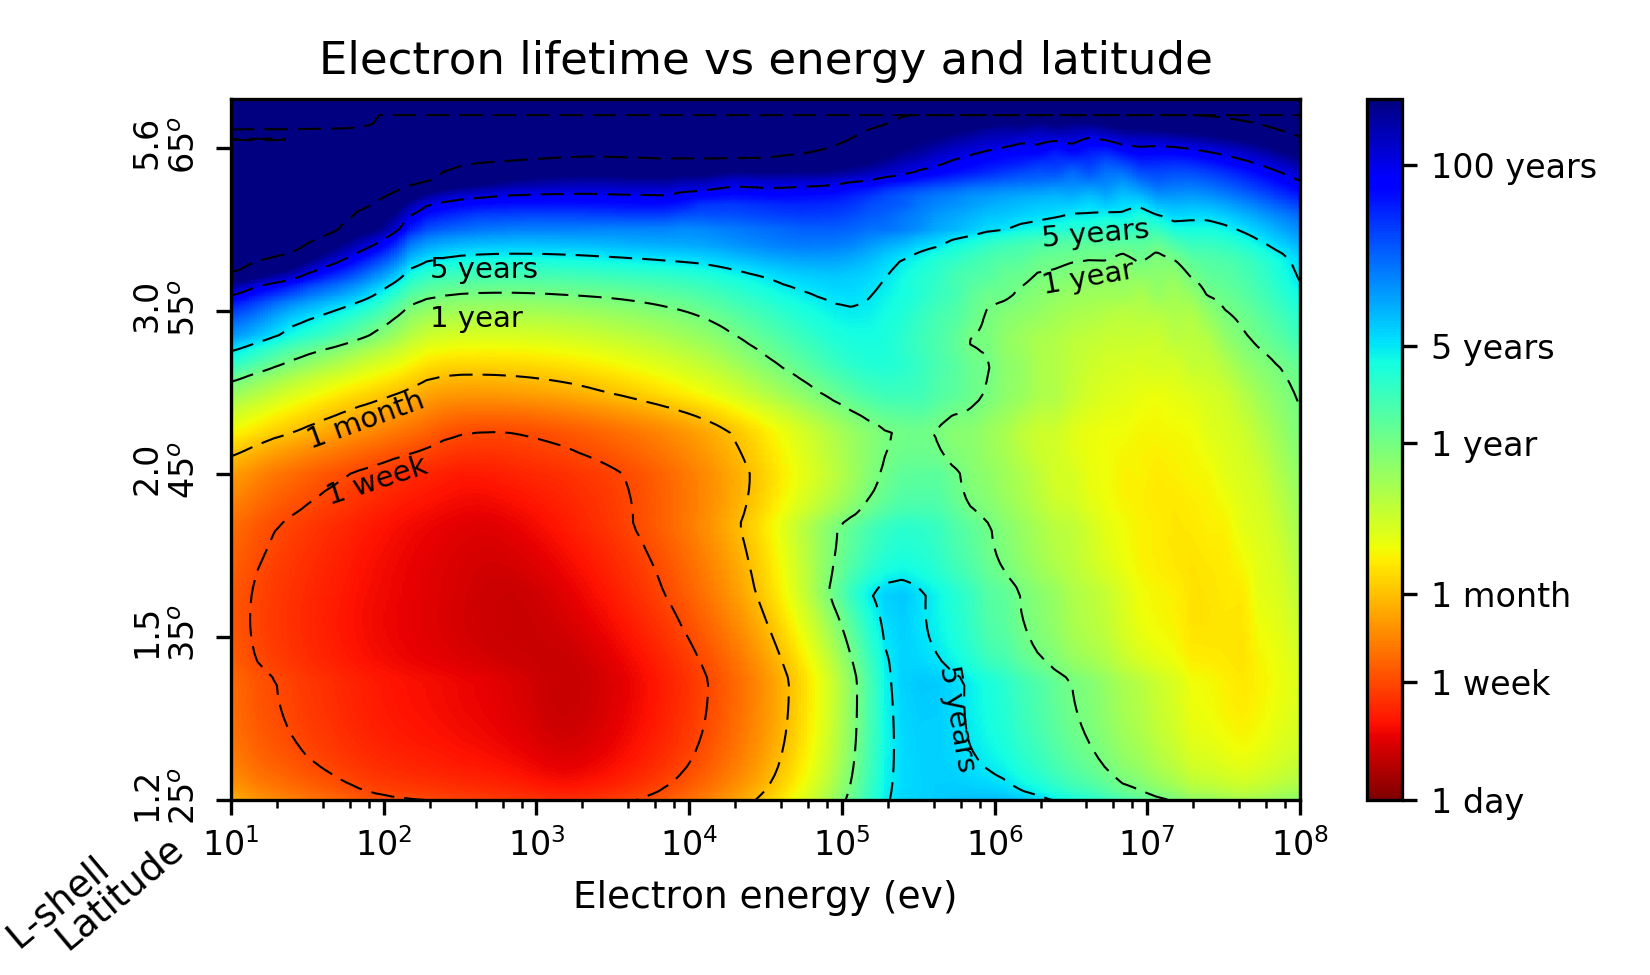
\includegraphics{figures/electron_lifetimes_updated_power_with_labels.png}
\caption[Estimated lifetime of radiation belt electrons subject to LEP losses only]{Estimated lifetimes ($\tau$, the time required for a population to decay by 1/e) for radiation belt electrons subjected solely to LEP-induced losses.}
\label{fig:electron_lifetimes}
\end{center}
\end{figure}


\section{Comparison to other research}
We can compare our resulting precipitation estimates to two related works: \cite{Gemelos2009} used data from the DEMETER spacecraft, along with seasonal lightning fluxes as measured by the NLDN network, to examine seasonal trends in LEP at 126 keV, and \cite{Meredith2007}, which uses \emph{in situ} VLF wave measurements to estimate lifetimes of radiation belt electrons due to various scattering mechanisms (LEP, chorus, hiss), using an incoherent interaction model.

Figure \ref{fig:gemelos_comparison} shows our modeled electron precipitation at 123 keV for August and December, averaged over 2014 - 2017, along with the corresponding northern hemisphere lightning activity as measured by GLD360, to facilitate comparison with \cite{Gemelos2009}, Figure 1. Geographically, our model shows very good agreement with \citeauthor{Gemelos2009}; however our modeled fluxes are several orders of magnitude lower. Possible explanations for the discrepancy in precipitation amplitude are that the DEMETER spacecraft orbited at 710 km altitude, while our fluxes are estimated at 100 km. Additionally, the DEMETER particle detector viewed particles with local pitch angles near $\sim 85^\circ$, and a full-width, half maximum viewing angle of $30^\circ$. Both \citeauthor{Gemelos2009} and \cite{Sauvaud2006} state that at this orientation the detector measures particles within or near the \emph{drift} loss cone, which may be considerably shallower than the bounce loss cone as modeled by our work.

\begin{figure}[]
\begin{center}
\includegraphics{figures/Gemelos_comparison.png}
\caption[Precipitation at 123 keV over the continental United States, for summer and winter]{Average precipitation at 123 keV over the continental United States, for summer (August) and winter (December). The bottom plots show the corresponding northern-hemisphere lightning as measured by GLD360.}
\label{fig:gemelos_comparison}
\end{center}
\end{figure}

Figure \ref{fig:Meredith_comparison} compares our estimated electron lifetimes to those reported by \cite{Meredith2007}. \citeauthor{Meredith2007} estimates electron lifetimes using a database of magnetosphere VLF wave measurements from the CRRES spacecraft; they then compute pitch angle scattering using the PADIE code, for a variety of assumed wave conditions. \citeauthor{Meredith2007} concludes that pitch angle scattering due to magnetospherically-reflecting whistlers (e.g., LEP) is of little relevance to relativistic electron lifetimes. However, \citeauthor{Meredith2007} uses an incoherent, quasilinear diffusion model, and therefore may not capture the effects of resonant pitch-angle scattering.

Our work is somewhat consistent, in that within the specified energy band, both works show lifetimes much greater than expected, suggesting that LEP is not a dominant loss mechanism. However, our model does show shorter lifetimes at lower L-shells. Additionally, \citeauthor{Meredith2007} does not examine lifetimes of lower energy electrons, for which our model shows the strongest losses. 
\begin{figure}[]
\begin{center}
\includegraphics{figures/Meredith_comparison_thesis.pdf}
\caption[Electron lifetime estimates compared against \cite{Meredith2007}]{Comparison of estimated electron lifetimes with those of \cite{Meredith2007}. Red lines show our results; blue lines show \cite{Meredith2007} estimates for quiet geomagnetic conditions; and orange for active geomagnetic conditions. Dashed black lines indicate the approximate measured lifetime of electrons (1 to 10 days).}
\label{fig:Meredith_comparison}
\end{center}
\end{figure}



    \chapter{Satellite Instrumentation for LEP Measurement}
        \label{chapter:VPM}
    	Having discussed the various steps in the LEP process, and the nuance required in modeling, we now turn to a more practical discussion, regarding direct measurement of pitch angle scattering due to wave-particle interactions. 

In the first few years of my time at Stanford, I worked on a hardware design for a CubeSat-based measurement platform, designed specifically for the study of these interactions. CubeSats are a class of nanosatellite, with a form factor made up of one or more 10-cm units (typically 3 units, and increasingly 6 units per satellite). Originally developed in 2000 as a classroom exercise, CubeSats have gained substantial popularity for university-scale missions, due to their comparably low development and launch costs \citep{Heidt2000}. CubeSats can ``piggyback'' onto larger commercial rocket launches, or be deployed from the Poly-Picosat Orbital Deployer (P-POD) aboard the International Space Station. A thriving, international ecosystem of CubeSats and associated products now exist, from university-scale missions, to government-sponsored projects, to commercial startups deploying large constellations of distributed sensors \citep{Woellert2011, Swartwout2013}.

Our project, named the VLF Wave-Particle Precipitation Mapper (VPM), formed a nexus of several research projects within the Stanford VLF group -- numerical modeling, fault-tolerant chip design, and embedded systems development -- and granted our small team of graduate students and research scientists design experience for a space-based mission. VPM was designed to provide simultaneous measurements of electron pitch angle distributions and incident whistler waves, in order to provide direct and quantitative measurements of whistler-induced pitch angle scattering efficiency.

In order to quantify the relative effect of waves on particle distributions, one needs to measure two quantities: The incident wave, in the form of electric and magnetic fields, and the pitch angles of the particles impinging on the satellite. VPM samples the wave by measuring two of the six wave components -- one $E$ and one $B$ field measurement, perpendicular to each other -- and the electron pitch angle distribution using two energetic particle spectrometers, oriented such that one samples only particles within the loss cone, and the other only trapped particles.

The VPM team was led by Dr. Robert Marshall and Dr. Ivan Linscott; the bulk of the hardware design was done by Jeff Chang and Steven Ingram. Additional software and hardware design was done by Christopher Young, Jordan Lenoach, and Alex Cousland. My primary contribution was the design and implementation of all the onboard firmware and digital signal processing. Design of the electron pitch-angle spectrometer system was contracted to a group at Lockheed Martin.

%One disclaimer to those embarking on a CubeSat design, or other space-based system: It seems to me that the final design of a project is dictated as much by well-intentioned engineering practices as it is by the constraints levied on the project. 
The design was dictated by two primary constraints: 1) design with the ability to exchange all commercial-grade components with space-rated components, and 2) in an effort to reduce the risk of catastrophic computer failures, to include no embedded firmware or programs stored in volatile memory. These constraints left a marked imprint on our final design. In a sense, we designed for a conventional satellite mission, with the notable exception that our instrument was small.

It is worth noting, however, that CubeSat missions generally fly in low-earth orbit ($\sim 400$ km altitude), and have mission lifetimes on the order of a few years, at maximum, due to atmospheric drag. While the idea of a fully radiation-tolerant design is alluring, it is hard to justify the price increase in parts (often $\sim 1000$ times greater than commercial, off-the-shelf components), and the difficulty in designing for them, for a short-duration, academic mission. To future students exploring potential CubeSat designs, I would advocate sacrificing bulletproof reliability in exchange for rapid design and prototyping, and affordability of flight components. Of course, a more-exotic mission such as an interplanetary probe or an asteroid orbiter would very much benefit from a fault-tolerant design.

The initial VPM prototype was delivered to the Air Force Research Lab (AFRL) in January, 2015. Both VPM and DSX were delayed several years afterward; as of this writing, VPM has been scheduled to launch in January, 2019.

\section{VPM Mission Overview}
The VLF Wave and Particle Precipitation Mapper (VPM) is a 3U CubeSat designed to measure wave activity and relativistic electrons in the Earth's radiation belts from low-Earth orbit (LEO). The VPM payload consists of an electric field dipole antenna and a magnetic field search coil to measure waves in the VLF frequency band from 100 Hz to 30 kHz; and two electron detectors, designed to measure electron energies from 100 keV to 1 MeV. In addition to single-spacecraft scientific goals outlined below, VPM is a companion to the Wave-Induced Precipitation of Electron Radiation (WIPER) experiment on the Demonstration and Science Experiments (DSX) mission \citep{Schoenberg2006, Spanjers2006}, a small spacecraft designed to investigate the Earth's radiation belts using active probing techniques. Both spacecraft are scheduled to be launched in 2019.

VPM will study the Earth's radiation belts from Low-Earth Orbit (LEO). The radiation belts are comprised of relativistic electrons from hundreds of keV to tens of MeV, and protons from tens to hundreds of MeV. As described in Chapter \ref{chapter:introduction}, these energetic particles can be highly damaging to spacecraft and to astronauts \citep[e.g.][]{Barth2003}, and comprise a vital component of space weather which affects satellite navigation and communication \citep{Bothmer:2007}. The distribution and evolution of radiation belt populations are controlled by geomagnetic activity and by wave activity in the plasmasphere. Radiation belt particles can be scattered in energy and pitch angle by magnetic reconfiguration, and by wave activity, which can include Alfvenic, electrostatic and electromagnetic waves. Waves can energize these particles, or cause them to precipitate and be lost to the Earth's upper atmosphere. The extent to which wave activity of different sources controls radiation belt distributions and lifetimes is still under considerable investigation. For example, the Van Allen Probes (VAP) mission, launched in 2012, is investigating the processes that accelerate and transport radiation belt electrons; radiation belt loss mechanisms; and the effects of geomagnetic storms on the radiation belts \citep{Spence2014}. %, Lanzerotti:2013 

Specific science goals of the VPM mission are:

\begin{enumerate}[noitemsep]
\item Improve climatology models of plasmaspheric hiss
\item Conduct conjunction experiments with the DSX mission and WIPER instrument
	\begin{enumerate}[noitemsep]
	\item Measure the Antenna Radiation Pattern of the WIPER VLF transmitter known as the TNT (Transmitter, Narrow-band receiver, and Tuners)
	\item Measure the Radiation Efficiency of the TNT
	\item Estimate the efficiency of wave-particle interactions using WIPER-injected waves
	\end{enumerate}
\item Improve understanding of the effects of lightning in the near-Earth space environment
	\begin{enumerate}[noitemsep]
	\item Improve climatology models of lightning and whistler activity
	\item Estimate the efficiency of lightning whistler-induced wave-particle interactions
	\end{enumerate}
\item Improve understanding of the effects of VLF transmitters in the near-Earth space environment
	\begin{enumerate}[noitemsep]
	\item Measure the efficiency of propagation in the earth-ionosphere waveguide and leakage into the ionosphere and magnetosphere
	\item Estimate the efficiency of VLF transmitter whistler-induced wave-particle interactions
	\end{enumerate}
\item Measure the trans-ionospheric absorption of lightning-generated sferics and whistlers
\item Measure VLF wave propagation characteristics in the near-Earth space environment
\item Validate models of wave-particle interactions
\end{enumerate}


Here we present the design of the VPM payload instrumentation and data processing, with an emphasis on the VLF wave instrumentation and data processing unit. The VPM payload is unique in a number of ways: i) four science instruments have been collocated in 1.5U of payload space; ii) all data processing is handled in firmware, reducing the power requirements and eliminating any software from the payload; and iii) data products are delivered with maximum flexibility thanks to the unique implementation of processing methods.


\begin{figure}[t]
\begin{center}
\includegraphics[width=20pc]{figures/vpm_figures/payload_figure_annotated.png}

\caption[Drawing of the assembled VPM payload on a 6U cubesat bus]{Drawing of an assembled VPM payload, shown in one possible configuration integrated into a 6U CubeSat bus, with both antennas deployed. Conical shapes indicate fields of view of the Loss Cone Electron Spectrometer (LES) and the Trapped Electron Spectrometer (TES). }
\label{fig:VPM_full}
\end{center}
\end{figure}

\begin{figure}[t]
\begin{center}
\includegraphics[width=20pc]{figures/vpm_figures/operations.png}

\caption[On-orbit alignment of the VPM payload]{Illustration of on-orbit alignment of the VPM payload. Conical, salmon-colored shapes indicate fields of view of the electron spectrometers; E and B fields are sampled perpendicular to each other and to the background magnetic field.}
\label{fig:operations}
\end{center}
\end{figure}




\section{Hardware Architecture}
VPM's system design was governed by three primary constraints:
\begin{enumerate}[noitemsep]
\item Facilitate integration with a 3U CubeSat bus. The payload must fit into a 1.5U (10 $\times$ 10 $\times$ 15 $\times$ cm) volume. The bus provides 3.3V and 5V power rails, an RS422 serial data communication connection, and a single, 1-Hz-sampled analog connection.
\item Provide an upgrade path for high-reliability, radiation-tolerant components wherever possible.
\item Design simple operation modes with high reliability and low verification complexity. 
\end{enumerate}

\noindent The VPM payload consists of five hardware systems:
\begin{enumerate}[noitemsep]
\item A power and interface board;
\item A two-channel VLF broadband receiver ($\mu$BBR);
\item Two deployable VLF antennas for sampling the electric and magnetic field respectively;
\item A digital data processing system (DPU);
\item and a Loss-Cone Spectrometer (LCS), a pair of electron energy spectrometers designed to sample the energy distribution of the local loss cone. 
\end{enumerate}
All circuit boards are connected by a common stack connector and housed in an aluminum enclosure to reduce parasitic RF interference. A rendering of the system is shown in Figure \ref{fig:hardware_stack}.

\begin{figure}[t]
\begin{center}
\includegraphics[width=32pc]{figures/vpm_figures/payload_figure.png}
\caption[VPM payload hardware instrument arrangement]{Rendering of the VPM payload hardware, showing locations of the E and B-field antenna deployers; the two particle detectors for the Loss-Cone Spectrometer, and the electronic card stack, shown without aluminum enclosure.}
\label{fig:hardware_stack}
\end{center}
\end{figure}


\subsection{FPGAs}
Full-scale space systems commonly use radiation-tolerant, multiple-redundant single-board computers. While robust and flight-verified, such systems are cost, size, and power-prohibitive for a CubeSat mission. Several commercial CubeSat single-board computers exist (such as those from Pumpkin or Tyvak); however these systems are designed for general satellite operations, and provide more functionality than necessary for an isolated payload. Additionally, single-CPU solutions are not well-suited for real-time, parallel streaming tasks, as data from multiple sources must be buffered and processed serially, increasing memory and clock speed requirements. VPM omits any such embedded CPU and instead uses a realtime streaming solution implemented entirely in a Field-Programmable Gate Array (FPGA). 

FPGAs consist of a network of assignable logic gates and interconnections, which allow for gate-level circuits to be implemented using a hardware development language such as VHDL or Verilog, achieving ASIC-like performance without the burden of IC development. By working at the gate level, multiple-input designs can operate in clock-cycle-accurate lock step, allowing for low-power designs with minimal wasted circuitry. Additionally, gate-level designs inherently have fewer operating states, and once implemented, provide a high degree of reliability without risk of segmentation faults, memory leaks, or other higher-level issues common in CPU systems.

FPGAs find common use in embedded systems for peripheral interfacing and low-level data handling. A hybrid CPU / FPGA design was considered, wherein a ``soft" CPU is implemented within the FPGA fabric -- however such a design needlessly increased verification complexity, while similarly reducing system reliability. It should be noted, however, that the VPM instrument acts only as a peripheral for a separate satellite bus, and is not tasked with a myriad of other responsibilities required of a satellite mission -- telemetry, communication, power management and so forth -- the complexity of which would necessitate a full CPU solution.

VPM uses the Actel ProAsic3 series of FPGAs. Actel FPGAs were selected largely for their focus on reliability, and simple upgrade path to a radiation-tolerant model. Development and prototyping was done using an A3PE/3000 chip (the largest available at time of design), which provides 3 million gates assignable in 75,264 tiles, and 604 kilobits of onboard SRAM. Additional functionality onboard the ProAsic3 series includes clock conditioning circuits, differential signaling drivers, and 1 kilobit of flash ROM used to store lookup tables, which combined allow for a single-chip data processing system. %\citep{actel_a3pe_datasheet}.


\subsection{Power and GPS}
The lowest circuit board in the VPM stack houses power systems, antenna deployer drivers, and a GPS daughterboard. VPM requires three power connections from the host spacecraft: +5V, +3.3V, and an unregulated, high-current-capacity supply at $\sim$ 9v, on a single micro-D connector. Additional connections are provided for two antenna deployers. A 100-pin stack connector is used for all inter-board power and communication.

VPM contains two deployable antennas: a 1-meter flexible dipole antenna for sampling the electric field, and a magnetic-field search coil, which is deployed away from the system to reduce parasitic noise. Both antennas are tensioned and held in place using a burn-wire deployer in which a thin plastic filament is held against a conductive wire. To deploy, VPM drives a current through the wire until the plastic filament melts through, allowing the antenna to unfurl without additional power, via stored tension.

The power and GPS board contains two drive transistors to provide the necessary burn-wire current, and are fed from the unregulated supply. Connections are made to deployers via a pair of micro-D connectors. Bipolar $\pm$ 12V power for the loss-cone spectrometer and searchcoil preamp is provided via a Picosat DC/DC converter. % \citep{picosat}. 

GPS timing and location are provided by a NovAtel OEM719 embedded GPS receiver. While not radiation-tolerant, this card has flight heritage on multiple CubeSat and nanosatellite missions, and can be configured to operate without altitude restrictions \citep{Spangelo2013}. Additionally, the OEM719 provides a GPS-disciplined sampling clock, which assures sample-accurate timing.

\subsection{DPU}
Data processing and system commanding is performed on the DPU board. The DPU board contains a single Actel A3PE/3000 FPGA housed in an FG484 ball grid array package. Local power for the FPGA is supplied by linear regulator circuits: 3.3V and 2.5V for IO banks, and switchable 1.5V or 1.2V for the FPGA core voltage, depending on whether an A3PE or A3PL part is populated. The FPGA is programmed through a 10-pin JTAG header.

Clocking onboard the DPU is provided by a 20 MHz temperature-controlled oscillator, which feeds a clock-conditioning circuit on the FPGA. Processing is done at a divided 10 MHz clock, with the exception of memory operations which operate at full speed.

Temporary data storage is provided by a 3D-Plus 128-megabyte SDRAM, which is clocked and controlled by firmware within the FPGA. The 3D-Plus SDRAM was selected primarily for availability of a pin-compatible, radiation-tolerant upgrade. The SDRAM uses a 32-bit wide data bus, and includes an internal refreshing algorithm.

Communication between VPM and the host satellite is implemented using a standard UART protocol over an RS422 connection, made through a pair of differential line drivers, again selected for a pin-compatible radiation-tolerant upgrade. % \citep{intersil_linedrivers}

VPM provides low-level housekeeping and debug signals over an analog connection, intended to be sampled by the host spacecraft. A variety of signals are connected through an analog multiplexing chip, including analog and digital power rails; system temperature as measured by a thermocouple near the GPS receiver; the bipolar 12V supply; and five channels allocated to the loss-cone spectrometer. Outputs can be selected via a system command, or set to cycle through at 5 seconds per input.

RS422 and analog housekeeping connections are made through a single micro-D connector. Connections are provided for an FTDI UM232H USB interface used extensively in development; however on flight, all connections are made through micro-D connectors or the 100-pin stack connector.

\subsection{VLF Receiver Boards}
VPM uses a modified version of the Stanford Micro Broadband Receiver ($\mu$BBR) as used on the SpriteSat mission, and the GLIMS payload onboard the International Space Station \citep{Ushio2011}. The VPM $\mu$BBR provides two channels of amplification, filtering, and digitization at an 80 kHz sampling rate. VPM uses a pair of proprietary chips -- a combination low-noise amplifier (LNA) and anti-ailiasing filter (AAF), and an analog-to-digital converter (ADC) -- which were the result of two Stanford PhD theses \citep{Wang2009, Mossawir2009}. The chips were designed for low power consumption and high radiation tolerance.

An intermediate buffering stage provides an additional 10 V/V gain; an active two-pole high-pass filter with a 3-dB point at 3 kHz can be inserted between the LNA and ADC sections, or bypassed completely using sealed, mechanical relays. Gain at the LNA can be remotely selected, either 1 or 10, for a total system gain of 20 or 40 dB. The assembled system gives a spurious-free dynamic range (SFDR) of approximately 55 dB across the passband. The analog stage operates on a single, 2.5V supply, which is derived locally using a 2.5V reference source and a radiation-tolerant op-amp. A simplified schematic of the receiver chain is shown in Figure \ref{fig:ubbr_schem}.

\begin{figure*}[t]
\begin{center}
\includegraphics[width=35pc]{figures/vpm_figures/ubbr_schem_with_preamps-2.pdf}

\caption{Simplified schematic of the $\mu$BBR signal conditioning and data conversion chain}
\label{fig:ubbr_schem}
\end{center}
\end{figure*}

Channel 1 features a differential input, which is capacitively coupled to the electric dipole antenna preamplifier. Channel 2 is single-ended, and connects to the output of a magnetic-field search coil, which contains its own active signal conditioning circuitry. Filtering and amplification is done differentially, using parallel single-ended circuits. 

The ADCs use a 5-stage pipeline architecture; digital assembly and calibration of the first three stages is performed in an FPGA. The resulting FPGA module returns 13-bit equivalent resolution, packed as 16-bit samples \citep{Wang2009}. 

Signal conditioning and ADC are located on a single board, which feed an interstitial FPGA on a second board. Parasitic coupling between the two channels is reduced by constraining each channel to a separate side of the board, with a ground-plane layer separating the two. 

The $\mu$BBR FPGA receives system and sampling clocks through the 100-pin stack connector, by way of the DPU FPGA. When enabled, the 80 kHz sampling clock is generated by the GPS card and is accurate to $\pm$50 nanoseconds. Should the system fail to detect a GPS-synchronized clock for more than 6 seconds, the system will attempt to reset the GPS card. If three resets are attempted without success, the system will default to an internally-generated sampling clock, which is derived from an onboard oscillator. GPS synchronization can be re-enabled via a system command.

All digital communication between the $\mu$BBR and the DPU is done via differential (LVDS) signaling. All communication is done synchronous to the DPU system clock, to eliminate communication errors due to clock and temperature drift.


 \subsubsection{Calibration Tone}
The $\mu$BBR signal chain features an onboard calibration signal generator, which can be used to assess the frequency response of the system on-orbit. A pseudorandom digital signal is generated using the $\mu$BBR FPGA, using the feedback register methodology described by \cite{Paschal2005}. VPM uses a 7-bit feedback register for a maximal-length sequence of 128 samples. This signal is passed through a voltage divider and capacitively coupled to the input of each analog channel. The Fourier transform of the resulting signal features a comb of uniformly-spaced frequencies, as shown in Figure \ref{fig:caltone}. When calibration mode is entered, the system will generate one minute of calibration tone, which can be recorded by a 30-second, full-resolution burst. Results of a typical calibration are shown in Figure \ref{fig:bbr_calibration}.

Finally, an onboard digital sine-wave generator can be enabled; in this mode the $\mu$BBR ignores any analog signal and delivers a full-scale sine wave. While not scientifically useful, this mode enables diagnosis of communications issues, and confirmation of survey-mode processing.

\begin{figure}[ht]
\begin{center}
\includegraphics[width=20pc]{figures/vpm_figures/caltone.eps}

\caption[Pseudo-random calibration signals]{Pseudorandom calibration signal. Plot (a) shows two repetitions of the signal in the time domain, with magnitude attenuated from the 3.3v LVDS pin; plot (b) shows the Fourier transform of the signal. Red circles denote total power summed from adjacent frequency bins, to account for windowing effects.}
\label{fig:caltone}
\end{center}
\end{figure}

\begin{figure}[t]
\begin{center}
%\includegraphics{Figures/gain_logfreq.eps}
%\includegraphics{Figures/noisefloor_logfreq.eps}
\includegraphics[width=20pc]{figures/vpm_figures/gain_noise_combined.eps}
\caption[Frequency response and noise floor of the $\mu$BBR analog processing chain]{Characteristics of the $\mu$BBR analog signal conditioning chain, beginning with the LNA/AAF.  Plot (a) shows the frequency response for both high and low gain settings. Responses of the antennas are not taken into account. Selectable high-pass filters are disabled. Plot (b) shows the power spectrum of the noise floor, which is effectively independent of gain setting. Level is in decibels relative to $\pm$ 1.0 volts full-scale.}
\label{fig:bbr_calibration}
\end{center}
\end{figure}



\subsection{Deployable Antennas}
VPM contains two deployable antenna structures, oriented perpendicular to each other and to the background magnetic field, which facilitate discrimination of electromagnetic waves from evanescent fields. The electric dipole antenna was designed by the Deployable Structures team at the Air Force Research Lab (AFRL), while the magnetic field antenna and apparatus was designed by the French Climate Research Laboratory at the National Center for Scientific Research (CNRS).

The electric dipole antenna is comprised of a conductive strip on a flexible tape, which is rolled up and held in place with a burn wire. 

%Analysis of an electrically-short dipole antenna in free space is straightforward and efficient: For an incident plane wave, the antenna can be modeled as an equivalent voltage source with $V=\|E_0\| sin(\theta)l_{eff}$, where $E_0$ is the magnitude and time-varying component of the electric field; $\theta$ is the angle between the wave vector and the antenna; and $l_{eff}=L/2$ is the effective length of the dipole element. This source is in series with an equivalent resistance given by:
%\begin{equation}
%R_{ant} = \frac{2 \pi}{3} \eta_0 (\frac{l_{eff}}{\lambda})^2
%\end{equation}

%where $\eta_0 = 377 \Omega$ is the characteristic impedance of free space, and $\lambda$ is the wavelength \cite{elliot_antennas}.

%Within the VLF band, the dipole resistance becomes trivially small. The antenna is capacitively-coupled to the $\mu$BBR input terminals, with a DC rolloff at 1 Hz. Assuming an infinite plane wave with right-angle incidence and ignoring plasma effects, the conversion between input voltage at the $\mu$BBR terminals and electric field magnitude $V_{in}/E_0$ (Volts per Volts / meter) is $\approx$ 1.

In the presence of a plasma, the electric dipole antenna's impedance can vary substantially with plasma parameters (density, temperature), and orientation with respect to the background magnetic field. For analytic, closed-form expressions, see \cite{Balmain1964}, and the series of papers by Wang and Bell \citep{Wang1969, Wang_Bell_1972}. For a full numerical treatment of plasma-immersed VLF electric dipoles, see the thesis work of \cite{Chevalier2007}. 

For purposes of system characterization, we assume the antenna and receiver are perfectly matched; assuming an infinite plane wave with right-angle incidence and ignoring plasma effects, the conversion between input voltage at the $\mu$BBR terminals and electric field magnitude $V_{in}/E_0$ (Volts per Volts / meter) is $\approx$ 1.

The search-coil antenna is also deployed from the payload to reduce electrical interference. The antenna includes a dedicated preamp which operates on $\pm$12V power. Sensitivity of the antenna and preamplifier are shown in Figure \ref{fig:searchcoil}.

Both antennas use a single-deploy burn-wire system. VPM includes options for each deployer to be armed and deployed separately, and can be repeated in the event that the retaining filament fails to release the antenna. Deployed antennas are shown in Figure \ref{fig:VPM_full}.

Figure \ref{fig:detectable_ranges} gives a rough estimate of the maximum and minimum detectable field amplitudes. Maximum levels are calculated assuming the low gain setting and a clipping voltage at the ADC; minimum levels are those which are below the system's noise floor at the high gain setting. Note that, for a plane wave in free space, the magnitudes of E and B are related by $B_0 = \frac{E_0}{c}$, where c is the speed of light; For an electric field $E_0 \approx 1$ V/m, the corresponding magnetic field has $B_0 \approx 0.3$ nT.

The range of measurable amplitudes is comparable to other in-situ VLF measurement systems; DEMETER reports a minimum sensitivity of $2\times10^{-5}$nT-Hz$^{-1/2}$ \citep{Cussac2006}. The Electric Fields and Waves (EFW) instrument onboard the Radiation Belt Storm Probes (RBSP) satellite use 100-meter double probe sensors with a maximum detection amplitude of $\pm 1$ V/m \citep{Wygant2014}. Several other studies report phenomena within the VLF band (whistlers, chorus) to have amplitudes on the order of 20 mV/m and 1 nT \citep{Wygant2014, Cattell2015, Bhattacharya2009}.



\begin{figure}[t]
\begin{center}
\includegraphics[width=20pc]{figures/vpm_figures/searchcoil_response_2up.eps}
\caption[Characteristics of the search coil and associated preamp]{Characteristics of the search coil and associated preamp. Plot (a) shows the transfer function in dB-scaled volts per nanotesla. Plot (b) shows the search coil and preamp's noise spectral density in units of $\mathrm{nT/Hz}^{1/2}$}
\label{fig:searchcoil}
\end{center}
\end{figure}


\begin{figure}[t]
\begin{center}
%\includegraphics{Figures/detectable_ranges.eps}
\includegraphics[width=20pc]{figures/vpm_figures/detectable_ranges.png}

\caption[Approximate detectable field magnitudes]{Approximate detectable field magnitudes, assuming no loss due to geometric factors of the antennas. Plot (a) shows the range of electric field strengths $E_0$ in Volts / Meter. Plot (b) shows the range of magnetic fields in nanotesla.}
\label{fig:detectable_ranges}
\end{center}
\end{figure}


\section{Firmware Architecture}
\begin{figure*}[t]
\begin{center}
\includegraphics[width=35pc]{figures/vpm_figures/firmware_diagram_v2.png}

\caption[Block diagram of VPM firmware modules]{Block diagram of firmware modules. Arrows indicate flow of data.}
\label{fig:firmware_arch}
\end{center}
\end{figure*}
VPM delivers two data products -- a low-resolution survey mode, which runs constantly, and a commandable burst mode, which will accumulate an equivalent of 30 seconds of full-resolution data. All data processing is performed on a single Actel ProAsic3 FPGA, using fixed-point, twos-compliment arithmetic. Survey and burst mode streams operate in parallel, feeding data to a common memory controller, which packetizes and buffers data using a radiation-tolerant 128MB SDRAM. Fixed-size packets are then transmitted at the soonest availability to the host spacecraft at 400 kilobaud using a standard RS422 / UART protocol. Figure \ref{fig:firmware_arch} shows a block diagram of the firmware architecture.


\subsection{Reduced-Resolution (Survey) Data}
Survey data consists of a reduced-resolution energy spectrogram for each VLF channel, and if installed, an energy histogram of each particle detector. Survey-mode time resolution can be selected from one of three presets -- short, medium, and long -- corresponding to 1024, 2048, or 4096 FFTs, or 6.5536, 13.1072, or 26.2144 seconds respectively. VLF spectrograms consist of 512 frequency bins, with energies mapped to 8 bits on a logarithmic scale.

\subsubsection{Frequency Mapping and Accumulation}
VLF data is delivered to the DPU as 16-bit, twos-compliment integers, which are buffered locally, overlapped by 50\% (512 samples), and multiplied by a Chebyshev window function. Data is then mapped to the frequency domain using a 1024-point, decimation-in-time Fast Fourier Transform, as described in \cite{Oppenheim_Schafer}. Buffering within the FFT is sized such that the full resolution of multiplications are kept without overflow. Real and imaginary components are rounded to 16 bits.

Absolute values of the real and imaginary components are then squared and summed, resulting in a 512-point vector of 32-bit integers, representing the squared magnitude of the frequency content.

Magnitudes are then accumulated using the full input resolution plus 12 padding bits, guaranteeing no overflow for $2^{12} = 4096 $ accumulations. The resultant output is a 512-point vector of 44-bit integers.

\subsubsection{Fixed-Point Log Scaling}
Arithmetic beyond addition, subtraction, multiplication, and power-of-two division is intractable without a dedicated arithmetic unit, generally requiring an iterative or multi-cycle algorithm. In many cases a simple lookup table can be used to map values from one space to another; however the size of a stored lookup table can become unwieldy with increased resolution. VPM makes use of a hybrid algebraic / lookup table method to map 44-bit integers to an 8-bit logarithmic space in a single clock cycle, and making efficient use of FPGA resources.

We begin with the log-of-sums identity:
\begin{equation}
\rm{log}_{n}(a + b) = \rm{log}_n (a) + \rm{log}_n(1 + \frac{b}{a})
\end{equation}
where we separate our input into the \emph{integer} portion, $a$, and the \emph{fractional} portion, $b$. We take the integer portion to be the maximum power of two less than the input, and the fractional portion to be the remainder, $b = x - a$. Each component can then be dealt with separately via a reduced lookup table.

The integer portion is simple to compute: $\rm{log}_2({2^{n}}) = n$, which can be calculated by finding the index of the greatest nonzero bit. To make full use of 8 output bits, we multiply by a scaling factor given by:
\begin{equation}
S = \frac{2^{Nb_{out}}}{Nb_{in}}
\end{equation}

Where $Nb_{out} = 8$, the number of bits at the output, and $W_{in} = 32$, the number of bits at the input, for a scaling factor of $S = 8$.

The fractional portion, $\rm{log}_2(1 + \frac{b}{a})$ is determined using a lookup table with $2^{Nb_{frac}}$ entries.

This method makes most-efficient use of the output range when both input and output bit widths are powers of two -- e.g., mapping 32-bit input to 8-bit output. Using $Nb_{in} = 32$, $Nb_{out} = 8$, and $Nb_{frac} = 5$, we require only two 32-entry lookup tables, rather than an intractable $2^{32}$ entries for a direct lookup table, or 256 entries for a partitioning lookup table.

VPM's accumulators deliver 44-bit integers, which must be passed into the 32-bit lookup tables. However, by simply taking the 32 most-significant bits, we introduce substantial error in the smaller output values. In order to make full use of the 44-bit integers, we use a barrel-shifting technique using the log-of-products identity:
\begin{eqnarray}
\rm{log}(ab) = \rm{log}(a) + \rm{log}(b) \\
\rm{log}(\frac{a}{b}) = \rm{log}(a) - \rm{log}(b) 
\end{eqnarray}

In the event that simply taking the most-significant 32 bits will result in a truncated fractional portion, we shift the input by $Nb_{frac}$ bits; equivalent to multiplying by $2^{Nb_{frac}}$. We then pass the top 32 bits to the lookup tables, sum the result, and subtract the added portion $S\cdot Nb_{frac}$. The complete module is shown in Figure \ref{fig:logscaling}, and performs within $\pm 1$ bit from the equivalent floating-point computation in Matlab when $x$ is greater than $2^{12} = 4096$.



For each frequency, the equivalent survey-mode computation is given by:
\begin{equation}
y_f = {\rm round}(S \cdot {\rm log}_2(\frac{1}{n}\sum_1^n{(\rm{re}(x_f)^2 + \rm{im}(x_f)^2)})
\end{equation}
where $x_f$ are the outputs of the windowed, overlapped FFT.


\begin{figure}[t]
\begin{center}
\includegraphics[width=20pc]{figures/vpm_figures/log2_v5.png}

\caption[Block diagram of the fixed-point log scaling module]{Block diagram of the log-scaling module, which efficiently maps a 32-bit average to an 8-bit value. Additional logic improves accuracy by making use of truncated bits for small inputs.}
\label{fig:logscaling}
\end{center}
\end{figure}

\subsubsection{Survey Product Data Structure}
\begin{figure}[h]
\begin{center}
\includegraphics[width=20pc]{figures/vpm_figures/survey_datastructure_column_v2.png}

\caption[Interleaving scheme for survey data]{Interleaving scheme for survey data. A single survey column consists of 512 bytes from each of the two VLF channels, 64 bytes from the spectrometer, and 180 bytes from the GPS receiver. The data are interleaved in four-byte segments.}
\label{fig:survey_data_format}
\end{center}
\end{figure}
Each column of the survey product includes a complete GPS timestamp containing time, location, and velocity. GPS timestamps are collected every second; however no provisions are made to snap columns to the exact start time. Rather, survey columns are transmitted every 1024, 2048, or 4096 FFTs, depending on current configuration, with the GPS timestamp corresponding to the last whole second before the column is requested. In order to eliminate storage requirements for staging a survey column, data from the VLF receiver channels are interleaved, along with data from the particle spectrometers if present, into a 4-byte output stream.

Each column begins with a 4-byte header, 0xABCD-1234. Survey data is then presented four bytes at a time, alternating between the two VLF channels and spectrometer data when available. The data stream alternates between the two VLF channels when the spectrometer data has been fully read out. When available, the survey data is followed by a 180-byte GPS timestamp. Each survey column ends with a four-byte footer, 0x6789-1234, and an appropriate number of zeroes to assure a complete 32-bit word is passed to the memory controller. When both GPS and spectrometer data are present, the resulting column is 1280 bytes. The data format is illustrated in Figure \ref{fig:survey_data_format}.

%Each column begins with a 4-byte header, 0xABCD-1234, followed by a 180-byte GPS timestamp (omitted when GPS timestamps are not available). Survey data is then presented four bytes at a time, alternating between the two VLF channels and spectrometer data when available. The data stream alternates between the two VLF channels when the spectrometer data has been fully read out. Each survey column ends with a four-byte footer, 0x6789-1234. When both GPS and spectrometer data are present the resulting column is 1260 bytes. The data format is illustrated in figure \ref{fig:survey_data_format}.



\subsection{Full-Resolution Burst Data}

VPM can log full-resolution data in a variety of modes, here referred to as \emph{experiments}. Data can be logged in either time or frequency domain, and can be taken on a modulated duty cycle, ranging from a single 30-second segment, to a selectable 1, 2, 5, or 10 seconds of data followed by a 2, 5, 10, or 30 second pause. The requested modulation will be repeated $nPulses$ times, which can be assigned via a separate command. When a GPS timestamp is available, an experiment will start at the next whole second after the burst command is received; if GPS card is not available, logging will start as soon as the command is received. Each subsequent on / off segment is tagged with a new GPS timestamp. A system status packet is logged at the beginning and end of each experiment.

Time-domain experiments can be taken at their full 80 kHz sampling rate, or decimated by factors 2, 4, 8, or 16. When decimation is selected, data is filtered using a 105th-order FIR low-pass filter. Filter coefficients were designed using the MATLAB Filter Design Toolbox (\emph{fdatool}), using the Least-Squares design algorithm. Cutoff frequencies were selected such that signals above the Nyquist frequency are attenuated by at least 60 dB. Filter coefficients are hard-coded and stored in on-chip ROM; filter delay lines are stored in on-chip RAM. Multiply-accumulate processing is done serially using a single hardware multiplier per channel. 

Maximum possible filter lengths are constrained both by available system resources, and by data sampling rate -- that is for each new data sample, we require $n$ multiplications. Given VPM's 10 MHz system clock and 80 kHz sample rate, a maximum filter is $\approx \frac{10e6}{80e3} = 125 $. $n=105$ was chosen to give sufficient padding for possible clock drift.

Frequency-domain experiments can be used to effectively reduce storage and transmission requirements in the event that only a small frequency band is of interest. The frequency range -- 512 bins, spaced uniformly between 0 and 40 kHz -- is split into 16 bands, which can be selectively enabled with each experiment. Each band contains 32 FFT bins for a bandwidth of 2500 Hz. VPM uses two parallel FFT engines, which implement a 1024-point FFT, using a 50\% overlap and a Chebyshev window function with 75 dB sidelobe attenuation. Frequency data is accurate to a MATLAB or similar floating-point FFT computation to within 16 bits. 

Burst experiments are selected using a 24-bit command structure as shown in Figure \ref{fig:burst_commands}. Each burst command begins with a header 2'b01. Bit three selects time-domain (1) or frequency-domain (0) data collection. Bit four enables time-axis duty-cycle modulation (``windowing"); bits 5 through 8 select the windowing pattern as shown in table \ref{tab:windowing}. For time-domain experiments, bit 9 enables downsampling and decimation. The downsampling factor is set by bits 10 and 11 -- 2'b00, 2'b01, 2'b10, and 2'b11 corresponding to 40 kHz, 20 kHz, 10 kHz and 5 kHz sampling rates respectively. For time-domain experiments, the remaining 13 bits are ignored. For frequency-domain experiments, bits 9 through 24 enable storage of each frequency band, from highest-frequency to lowest-frequency. 


\begin{table}
\centering
\caption[Burst mode duty cycle modulation settings]{Burst-mode duty-cycle modulation settings. Modes are listed as seconds on / seconds off.}
\label{tab:windowing}
\centering
\begin{tabular}{c|ccc|ccc|ccc|cc}
 0 & 10/30 & & 4 & 5/30 & & 8 & 2/30 & & 12 & 1/30  \\
 1 & 10/10 & & 5 & 5/10 & & 9 & 2/10 & & 13 & 1/10  \\
 2 & 10/5   & & 6 & 5/5   & & 10  & 2/5   & &  14 &1/5  \\
 3 & 10/2   & & 7 & 5/2   & & 11 & 2/2   & &  15 & 1/2  \\
\end{tabular}
\end{table}


\begin{figure}[t]
\begin{center}
\includegraphics[width=20pc]{figures/vpm_figures/burst_commands.png}

\caption[24-bit command structure for burst experiments]{24-bit command structure used to request burst experiments. The top row shows a time-domain experiment; the bottom shows a frequency domain experiment.}
\label{fig:burst_commands}
\end{center}
\end{figure}


\subsection{GPS Timestamps}
VPM uses a NovAtel OEM 615 embedded GPS receiver which communicates directly with the DPU via RS232. When the system is reset, or when GPS synchronization is selected, the DPU requests two data products -- BESTPOSB and BESTVALB -- which provide solutions for position and velocity, encoded in a binary stream. Timestamps are updated every second, and are accurate to the system sampling clock / PPS to $\pm 50$ ns. Together, the two data products occupy 180 bytes, and include position, velocity, and several metrics of quality-of-fit. Decoding can be done using the NovAtel Convert4 application, or our provided MATLAB script.

Figure \ref{fig:example_data} shows an example of a frequency-domain experiment, which has been windowed on both the time and frequency axes, and its corresponding survey data.

\begin{figure}[t]
\begin{center}
%\includegraphics{Figures/burst_example.eps}
\includegraphics[width=20pc]{figures/vpm_figures/burst_example.png}
\caption[Example of a frequency-domain burst experiment]{An example of a burst experiment. Plot (a) shows the data returned from a frequency-domain burst experiment, which has been windowed in time using mode 6 -- five seconds on, five seconds off. Only every other frequency bin has been enabled. Input to the $\mu$BBR is a 10-second frequency sweep. Plot (b) shows the corresponding survey data, using the highest-resolution setting ($\approx$ 6.5-second bins). The dashed black overlay shows the approximate input frequency. Amplitudes are shown in decibels relative to full-scale.}
\label{fig:example_data}
\end{center}
\end{figure}


\subsection{System Status Messages}
VPM includes provisions for a single, comprehensive system status message. A system status message is logged at the beginning and end of each burst experiment; at the beginning of an antenna arm or deploy command; if the GPS receiver times out; or upon request by the host spacecraft.

Status messages include the following information:
\begin{itemize}[noitemsep]
\item Source of the status request
\item Last command received by the system
\item System uptime in seconds
\item Total commands received by the system
\item Channel enabled / disabled status of E, B, and LCS burst data
\item Sampling clock selection - either GPS or internal
\item Deployer arm status for each antenna
\item Total attempted antenna deploys since last reset
\item Analog housekeeping mux setting
\item Survey product duration
\item Current burst repeat setting
\item Total packets sent from each data stream
\item Total bytes currently stored in memory
\item Current experiment number for each data stream
\item Total count of GPS errors and attempted resets
\end{itemize}
\subsection{Memory and Data Storage}
VPM lacks a full-fledged CPU and operating system, which necessitates the creation of a simple data handling and arbitration scheme. Use of a file system is avoided by regarding pre-transmission memory as a single buffering queue, with the expectation that data is read by the host spacecraft at the soonest availability. Memory management is divided into a set of packetizing modules -- one for each unique datastream -- which feed a simple arbitrating state machine. Complete packets are then stored contiguously in the external 128 MB SDRAM in the order in which they are generated. Packets are read contiguously, first-in-first-out. 

\subsubsection{Packeting}
VPM has facilities for six unique datastreams: Survey data; two channels of VLF data; spectrometer (LCS) data; GPS timestamps; and system status messages. Each datastream feeds an identical parallel packeting module, which writes packet headers and footers, logs metadata required in decoding, escapes header bytes from within the datastream, and inserts padding zeros to guarantee a consistent 512-byte packet. Packeting modules can each buffer two full packets before being read out.

Header and footer bytes are both 0x7E; however bytes in the datastream can take on all possible values between 0x00 and 0xFF. To prevent confusion when reading packets, we escape all instances of 0x7E within the datastream and insert a two-byte sequence 0x7D7D. Additionally, instances of 0x7D are replaced with 0x7D5D. To guarantee realtime streaming, escaping and external SDRAM reads and writes operate on a full-speed 20 MHz clock. 

VPM's packet structure is shown in Figure \ref{fig:datastructure}. The following metadata are included in each packet:
\begin{itemize}
\item Packet Start Index (4 bytes): A four-byte integer representing the sample index of the first value within the packet -- used in assembling many thousands of packets from a burst experiment into a contiguous field.
\item Data Type (1 byte): Each channel is tagged with a single-byte label, denoting the packet's source: ASCII ``S" for Survey; ``E" for VLF 1; ``B" for VLF 2; ``L" for spectrometer data; ``G" for GPS data; and ``I" for system information / status messages.
\item Experiment Number (1 byte): Each experiment or survey column share a common experiment number, used to distinguish packets from sequential experiments.
\item Checksum (1 byte): A simple checksum is provided as a quick verification of packet health. VPM's checksum is a simple, 1-byte rolling sum of all prior bytes in the packet, including headers and escape characters. Two bytes are reserved in the packet order so that, in the event that the checksum value is escaped, the packet will remain a fixed size.

\item Byte Count (2 bytes): An integer representing the number of bytes contained within the packet, post-escaping. In order to maintain a fixed-size packet, data fields are padded with a variable number of zeroes. Three bytes are reserved for Byte Count in the event that the value is escaped. Note that only one value need be reserved, as the most-significant byte will never be escaped.
\end{itemize}

\begin{figure}[t]
\begin{center}
\includegraphics[width=20pc]{figures/vpm_figures/packet_structure_column.png}

\caption[Structure of packets returned by VPM]{Structure of packets returned by VPM. Packets include various metadata required for reassembly, and are zero-padded to assure a constant size of 512 bytes.}
\label{fig:datastructure}
\end{center}
\end{figure}

\subsection{System Control}
Commands are passed to VPM through the RS422 port, which operates at 400 kilobaud. Commands are received by a simple format-checking state machine. All commands are 24-bit, and of the form: $\{$ 0x7E $\|$ Byte 1 $\|$ Byte 2 $\|$ Byte 3 $\|$ 0x7E$\}$. Bytes are reassembled in big-endian order. Commands which do not meet this form exactly are discarded; however, the three command bytes must be escaped in the same manner as on transmission if they include a 0x7E or 0x7D value.

Successfully-received commands are passed to a master state machine, which then sets global parameters and passes commands to submodules accordingly.

The first two bits of a command dictate the intended recipient: 2b'00 for DPU and system commands; 2b'01 for burst commands; 2b'10 for $\mu$BBR commands; and 2b'11 for commands sent to the loss-cone spectrometer.

DPU commands are in a human-readable ASCII character format (``G1" = Enable GPS, ``G0" = Disable GPS, etc). Burst and $\mu$BBR commands assign a specific purpose to each of the remaining 22 bits.


\section{Concluding Remarks}
We have described a novel design for a CubeSat payload instrument, which is capable of sampling the VLF band of the electromagnetic spectrum while simultaneously sampling energetic particle distributions of the radiation belt. The system draws less than 5 Watts including the onboard GPS receiver, and occupies a 1.5U volume. The system provides two data products -- a low-resolution survey product which runs continuously, and a full-resolution burst product, which is available on demand from the host spacecraft. The onboard software is implemented entirely in an FPGA fabric, eliminating the need for additional volatile program storage, which reduces risk of CPU errors and improves system reliability. Additionally the system can be implemented using radiation-tolerant components. A CubeSat carrying the VPM payload is scheduled to be launched by the Air Force Research Laboratory in 2019.





    \chapter{Conclusions}
    	Over the preceding chapters we have examined the global impact of lightning-generated whistlers, and associated electron precipitation, on the ionosphere and radiation belts. 

In chapter \ref{chapter:power} we modeled the persistent radio energy within the plasmasphere and magnetosphere due to lightning-generated whistlers; the energy is generally confined by the plasmapause, inside which there is little variation with respect to geomagnetic conditions. We find that the persistent energy decays logarithmically with increasing L-shell, as in figure \ref{fig:energy_density_vs_L_trendline}. We find a similar logarithmic trend in the radio frequency spectrum, in which the average bandwidth of lightning-generated energy decreases with increasing L-shell, as in figure \ref{fig:energy_density_vs_L_vs_freq}.

Chapter \ref{chapter:global_estimates} built on the ray tracing and interpolation methodology of chapter \ref{chapter:power} to examine the global impact of LEP, both as a magnetosphere-ionosphere energy coupling mechanism, and as a radiation belt depletion mechanism. We consider energy deposition from maximally and minimally populated radiation belts. We capture the seasonally-varying morphology of \cite{Gemelos2009}, and are in reasonable agreement with \cite{Meredith2007} for electron average electron lifetimes in the MeV energy range. Our simulation finds that while LEP is not a significant loss mechanism for highly-relativistic electrons in either the inner or outer belts, we find LEP to be a highly significant loss mechanism for suprathermal (100 eV - 10 keV) electrons in the inner radiation belt. We do not find any notable enhancement in slot-region losses, suggesting that LEP is not significant in the depletion of the slot region. However, we consider only the first 20 seconds of a propagating whistler, after which significant energy in the middle frequencies and middle L-shells remain; as was theorized by \cite{Bortnik2005}, this energy likely evolves into incoherent plasmaspheric hiss, which has been surmised elsewhere to be principal driver of the slot region.

Chapter \ref{chapter:VPM} detailed the practical issues of a CubeSat-based VLF receiver, designed for \emph{in-situ} measurements of LEP. While the receiver was constrained by the power and volume requirements of a CubeSat, this system included additional constraints not normally addressed in microscale / university-level satellite design. These constraints include designing for radiation-tolerant upgrades in mind, which, while of small significance for short-duration, low-earth-orbit missions, may be of greater significance for highly-elliptical orbits or future CubeSat missions to planets and objects outside the magnetosphere. Additionally, the receiver was designed as a peripheral device, with no volatile software onboard, using the hardware description language VERILOG.

\section{Suggestions for Future Work}

\subsection{Model Improvements}
\paragraph{Ray Tracing}
The morphology of LEP is driven primarily by the paths of incident whistlers; within our modeling, these paths are defined through raytracing in a modeled plasmasphere environment. Numerous improvements could be made here, with possible new science of interest, as the detail and realism in plasmasphere modeling is increased. Driven by both for a desire to generalize, and a lack of computational resources, we artificially constrain our raytracing to the meridional plane (as defined by the Earth's magnetic field). Furthermore we had difficulty in balancing accuracy versus reasonable timestepping (reducing error tolerances would frequently reduce our timestep to picoseconds), which resulted in erroneous deviation along the longitudinal axis. Exploring alternatives to the Runge-Kutta ODE solver, as well as incorporating the warm plasma corrections of 
\cite{Maxworth2017} may serve to reduce these errors.
Generally, at noon and midnight local time, we expect minimal gradients along the longitudinal axis, and the meridional-plane constraint should hold. However, lightning generally occurs around dusk and dawn (as in figure \ref{fig:Io_and_MLT}), where there may likely be stronger longitudinal gradients, which could impart a significant spreading or offset to the precipitation stencils of chapter \ref{chapter:global_estimates}. % different solvers, etc, etc, warm plasma effects, etc etc.

\paragraph{Interpolation and Granularity}
The energy and precipitation stencils could each benefit from a finer granularity in guide rays, and from finer frequency steps in interpolation. An additional, reasonably-straightforward modification to our interpolation scheme would be to consider the \emph{concave hull} mentioned in figure \ref{fig:convex_hulls}. Our interpolation algorithm at present assumes a convex hull, which will always span a volume equal or greater to the concave hull.

\paragraph{Backscatter and Altitude Effects}
Our precipitation codes do not include the Atmospheric Backscatter model of \cite{Cotts2011}; \citeauthor{Cotts2011} finds that a significant fraction of electrons bounce back after penetrating below 100km altitude (below which our model considers a particle to be lost). The rebounded particles may then interact with additional VLF wave activity, and possibly precipitate into the opposite hemisphere.

Of interest for transmitter-based measurements of LEP would be a more-thorough treatment of precipitating depth. As noted in \cite{Cotts2011}, there is a significant difference in precipitation likelihood between `grazing' precipitation and `deep' precipitation. Furthermore, the lower-energy, suprathermal electrons which comprise the bulk of our precipitation energy estimates likely precipitate at higher altitudes; VLF transmitter remote sensing techniques are sensitive dominantly to the lower edge of the ionosphere ($\sim$ 85 km), and may not be impacted by particles deposited closer to our 100 km threshold.
% raytracer improvements
% Incorporation of Atmospheric Backscatter codes
% Consideration of absorption altitude (low-energy stuff gets driven down *hard*, but always precipitates closer to 100km -- insignificant for transmitter studies?

\subsection{Global Trend Improvements}
\paragraph{Correlation between Filling Conditions and K$_p$}
% Filling conditions -- higher kp = higher filling, but lower wave activity?
The dynamics the radiation belt are marked by short-duration, sporadic filling events. These filling events may coincide with increased solar activity (possibly with a delay), which in turn may result in a higher K$_p$. Within our work, we consider precipitation from maximally and minimally filled radiation belts. However, we find less precipitation at higher K$_p$ values, due to the constricting nature of the plasmapause. Incorporating measured / historical filling data along with GLD360 and K$_p$ data may result in a better estimate of energy deposition, rather than an upper or lower bound.

\paragraph{Coherent vs Incoherent Methods}
In chapter \ref{chapter:global_estimates}, we determine global electron precipitation by taking a scaled sum of individual, (pseudo) coherent precipitation events using GLD360. However, numerous work exists on incoherent diffusion methods \citep{Kennel1966, Lyons1973, Glauert2005}. Rather than summing the precipitation after interaction, one could use the power estimates from chapter \ref{chapter:power}, and feed the determined distributions into an incoherent diffusion code. Such an implementation would be an excellent comparison between the coherent and incoherent diffusion approaches, which generally treat different physical systems -- coherent for LEP, and incoherent for chorus and hiss.
% Comparison to PADIE codes, etc

\subsection{Related Phenomena}
\paragraph{Cloud-to-Cloud lightning}
Our study is constrained to lightning discharges measured by the GLD360 dataset, which is designed to detect Cloud-to-Ground only. However, Cloud-to-Cloud lightning may be a significant, additional source of whistler waves. The single-flash modeling used in computing the energy and LEP stencils could be easily adapted to model a cloud to cloud discharge; one would need only to provide a new model of illumination (see section \ref{section:input_power}). 
% cloud-to-cloud
\paragraph{Transmitter-induced Precipitation}
Similarly, the stencil computation method could be adapted to study precipitation resulting from VLF transmitters. In contrast to the impulsive, broadband whistlers generated by lightning, VLF transmitters provide a constant, narrowband signal. It has been theorized that the constant effect of numerous global transmitters constitutes an anthropogenic driver of the so-called ``impenetrable barrier'' for relativistic electrons \citep{Baker2014, VLF_BUBBLE}.
% power and precipitation estimates for VLF transmitters

% different lightning datasets -- detection efficiency?

% Comparison to real data!



   \appendix
   \chapter{Reference Equations}
    \section{Landau Damping}
\label{appendix:landau}

In raytracing, we calculate wave growth and attenuation according to Landau damping. We use the \citet{Brinca1972} formulation -- itself a reorganization of \cite{Kennel1966} -- which assumes a cold background plasma, onto which a small thermal electron population is ascribed. The following (frustratingly complex) equation set is taken from \cite{Brinca1972}, and reprinted here for organization.

Calculating a growth rate begins simply: we assume a time-varying plane wave in the usual complex (``phasor'') form:

\begin{equation}
E \sim E_0 \exp{i(\omega t - \vec{k}\cdot\vec{r})}
\end{equation}

If either $\omega$ or $\vec{k}$ have an imaginary component, then the result will be an additional real-valued term, which we can factor out as $\chi$:
\begin{eqnarray}
E & = &E_0 \exp{i( \omega t - (\vec{k_r} + i\vec{k_i})\cdot\vec{r})} \\
& = &E_0 \exp{-\chi r}\exp{i(\omega t + \vec{k_r}\cdot\vec{r})}
\end{eqnarray}

If the new exponential term $-\chi$ is positive, the wave will be amplified; if the term is negative, the wave will be attenuated.

The spatial growth rate $\chi$ is given by equation \ref{eqn:brinca_chi} \citep{Brinca1972,Kennel1966}:
\begin{equation}
\chi = -\frac{c k_i}{\omega} = \frac{\delta}{4 \eta (2 A \eta^2 - B)} \big( T_1 - T_2 - T_3 \big) \\ \label{eqn:brinca_chi} 
\end{equation}
with the following terms:

\begin{eqnarray}
&T_1 = & \frac{\eta^2\sin{\theta}^2 - P}{2(S - \eta^2)}\Gamma_I \cdot [(R - \eta^2)J_{m-1} + (L - \eta^2)J_{m+1}]^2 G_1 \\ \nonumber
&T_2 = & 2[(S - \eta^2 \cos^2\theta)(S - \eta^2) - D^2] \Lambda_I J_m G_2 \\ \nonumber
&T_3 = & 2\eta^2 \sin \theta \cos \theta \Gamma_I\cdot [(R - \eta^2)J_{m-1} + (L - \eta^2)J_{m+1}]G_2 \\ \nonumber
\end{eqnarray}

where $\chi > 0$ indicates damping.

Note that \citeauthor{Brinca1972} has related the temporal damping rate $\omega_i$ from \cite{Kennel1966} to a spatial damping rate $k_i$ by assuming a constant propagation at the group velocity $v_g$.

$A, B, C, D, L, P, R,$ and $S$ are the Stix environment parameters given by equations (\ref{eqn:stix_params_1} -- \ref{eqn:stix_params_2}), and are functions of wave frequency, local plasma density, and local magnetic field strength. 

$\theta$ is the angle between the wavenormal vector and the background magnetic field, and $\eta$ is the wave refractive index, found by solving equation \eqref{eqn:disp_rln}.

The terms $J_m, J_{m+1}$ and $J_{m-1}$ are Bessel functions of the first kind, which account for the multiple resonant modes; $m=0$ indicates the Landau resonance, while $m\pm1$ the Cyclotron resonance, with the sign denoting co-streaming (positive) or counter-streaming (negative) resonances. Higher order resonant modes remain unnamed. 

The terms $\Gamma_I$ and $\Lambda_I$ are summations over resonant modes $m\in \{-\infty...\infty\}$ , and integrations over the velocity space $v_\perp$,$v_\parallel$ given by:

\begin{eqnarray}
&\Gamma_I &= \frac{2\pi^2\omega_p^2}{\omega k_\parallel} \sum_{m=-\infty}^{\infty}\int_0^\infty v_\perp^2 dv_\perp \int_{-\infty}^\infty \delta(v_\parallel - V_m) d v_\parallel \\
&\Lambda_I &= \frac{2\pi^2\omega_p^2}{\omega k_\parallel} \sum_{m=-\infty}^{\infty}\int_0^\infty v_\perp dv_\perp \int_{-\infty}^\infty v_\parallel \delta(v_\parallel - V_m) d v_\parallel
\end{eqnarray}
\begin{equation}
V_m = \frac{\omega - m\omega_c}{k_\parallel}
\end{equation}

Finally, the temperature distribution is included in the values $G_1$ and $G_2$ -- each of which are functions of the \emph{gradient} of the phase-space distribution function:

 $f=f(\vec{x}, \vec{v}) = f(\vec{x}, v_\perp, v_\parallel)$:

\begin{equation}
G_1 = \bigg(1 - \frac{k_\parallel v_\perp}{\omega}\bigg)\frac{\partial f}{\partial v_\perp} + \frac{k_\parallel v_\perp}{\omega}\frac{\partial f}{\partial v_\parallel}
\end{equation}
\begin{equation}
G_2 = J_m\bigg[\bigg(1 + \frac{m \omega_c}{\omega}\bigg)\frac{\partial f}{\partial v_\parallel} - m \frac{\omega_c}{\omega v_\perp} \frac{\partial f}{\partial v_\perp}\bigg]
\end{equation}

Despite the complexity of these equations, the phase-space distribution function $f$ is the only fundamental new input -- every remaining parameter is an output of the raytracer, and itself a result of our plasma density and magnetic field models.

Our implementation, derived from \cite{Golden2010}, computes the gradients of $f$ numerically using finite differencing, therefore granting the flexibility to use any arbitrary distribution function.


%& = & \frac{\delta}{4 \eta (2 A \eta^2 - B)} \big\{\frac{\eta^2\sin{\theta}^2 - P}{2(S - \eta^2)}\Gamma_I \\ \nonumber 
    
    \chapter{Runge-Kutta Methods}
    \label{appendix:runge_kutta}

    \bibliography{library}
    \end{document}








 









Documentation: 
    This style file modifies the standard report style to follow the
    Graduate Degree Support Section of the Registrar's Office's
    "Directions for Preparing Doctoral Dissertations".  It sets the
    margins and interline spacing and disallows page breaks at
    hyphens.

    The \beforepreface command creates the title page, a copyright page
    (optionally), and a signature page.  Then the user should put
    preface section(s), using the \prefacesection{section title}
    command.  The \afterpreface command then produces the tables of
    contents, tables and figures, and sets things up to start
    the main body (on arabic page 1).
    
    The following commands can control what goes in the front matter
    material:
    
        \title{thesis title}
        \author{author's name}
        \dept{author's department}
                - Computer Science if omitted
The following switches allow for special title pages (not all are current)
        \committeethesis - for a thesis in a committee (no dept.)
                           use \dept{committee name}
        \programthesis - for a thesis in a program (no dept.)
                           use \dept{program name}
        \educationthesis - for the School of Education. \dept doesn't matter
        \businessthesis - for the GraduateSchool of Business. \dept doesn't matter
        \lawthesis - for the School of law. \dept doesn't matter
        \humanitiesthesis - for a thesis also submitted to the Graduate
                            Program in Humanities
        \specialthesis  - for a Graduate Special thesis
        \industrialthesis - for a thesis in Industrial Engineering
        \dualthesis     - for a thesis in a dual language department.
                          Also define \languagemajor{language}.
                          e.g., \dept{French and Italian} 
                          \languagemajor{Italian}
         \principaladviser{the principal advisor's name}
           (or \principaladvisor, if you prefer advisor spelled with o)
        \coprincipaladviser{optional second principal advisor's name}
           (or \coprincipaladvisor, use only if you have two principal
           advisors only for the second one)
        \firstreader{the first reader's name}
        \secondreader{the second reader's name}
        \thirdreader{optional third reader's name}
        \fourthreader{optional fourth reader's name}
        \setlength{\signaturespace}{.5in} 
                - default is .5in, can be adjusted to fit all
                signatures in one page
        \submitdate{month year in which submitted to GPO}
                - date LaTeX'd if omitted
        \copyrightyear{year degree conferred (next year if submitted
          in Fall quarter)}
                - year LaTeX'd (or next year, in December) if omitted
        \copyrighttrue or \copyrightfalse
                - produce or don't produce a copyright page (true by default)
        \thesiscopyrighttrue or \thesiscopyrightfalse
                - produces the style of copyright page listed by the
                Thesis Office or the style that everyone else uses
                (Thesis office by default).
        \figurespagetrue or \figurespagefalse
                - produce or don't produce a List of Figures page
                  (true by default)
        \tablespagetrue or \tablespagefalse
                - produce or don't produce a List of Tables page
                  (true by default)

This style uses interline spacing that is 1.3 times normal, except
in the figure and table environments where normal spacing is used.
That can be changed by doing:
    \setstretch{1.6}
(or whatever you want instead of 1.6)

This command should be put before the \begin{document} command but
after loading the packages

You can also set any particular section in singlespacing mode by using
the singlespace environment.  For example

\begin{quote}
\begin{singlespace}
...
\end{singlespace}
\end{quote}

makes the quote singlespaced.  See the documentation for setspace.sty
for more information.

The example at the beginning shows the 12pt substyle being used.  This
seems to give acceptable looking results, but it may be omitted to get
smaller print.